%! Author = Darie-Dragos Mitoiu
%! Date = 23/08/2020

% Preamble
\documentclass[12pt]{report}

\setcounter{tocdepth}{4}
\setcounter{secnumdepth}{4}

% Packages
\usepackage{amsmath}
\usepackage{graphicx}
\usepackage{geometry}
\usepackage[titles]{tocloft}
\usepackage[hidelinks]{hyperref}
\usepackage{bookmark}
\usepackage{lmodern}
\usepackage{indentfirst}
\usepackage{caption}
\usepackage[round, numbers]{natbib}
\usepackage{fancyhdr}
\usepackage{tabularx}
\usepackage{scrextend}
\usepackage{enumitem}
\usepackage{longtable}
\usepackage{listings}
\usepackage[acronym]{glossaries}
\graphicspath{images/}

\renewcommand{\contentsname}{Contents}
\renewcommand{\bibname}{References}
\renewcommand{\cftchapfont}{\normalfont\bfseries}
\renewcommand{\cftchappagefont}{\normalfont\bfseries}
\renewcommand{\arraystretch}{1.5}
\renewcommand{\lstlistingname}{Algorithm}% Listing -> Algorithm
\renewcommand{\lstlistlistingname}{List of \lstlistingname s}% List of Listings -> List of Algorithms

\setlength{\tabcolsep}{0.5em}

\geometry{
    paper=a4paper, %        Change to letterpaper for US letter
    inner=2.5cm, %          Inner margin
    outer=3.0cm, %          Outer margin
    bindingoffset=.5cm, %   Binding offset
    top=1.8cm, %            Top margin
    %showframe, %           Uncomment to show how the type block is set on the page
}

\AtBeginDocument{
    \hypersetup{pdftitle=A Desktop Application for Maintenance of Computer Systems}
    \hypersetup{pdfauthor=Darie-Dragos Mitoiu}
    \hypersetup{pdfkeywords=Computer Systems Maintenance}
}

\author{Darie-Dragos Mitoiu}

\fancyhf{}
\fancyhead[RE]{\chaptername~\thechapter}
\fancyhead[LO]{\leftmark}

\fancyfoot[C]{\thepage}

\pagestyle{fancy}

\makeglossary
%! Author = Darie
%! Date = 17/04/2021

\newacronym{cpu}{CPU}{Central Processing Unit}
\newacronym{cpus}{CPUs}{Central Processing Units}
\newacronym{ram}{RAM}{Random Access Memory}
\newacronym{rom}{ROM}{Read-Only Memory}
\newacronym{hdd}{HDD}{Hard-Disk Drive}
\newacronym{smart}{S.M.A.R.T}{Self-Monitoring Analysis and Reporting Technology}
\newacronym{ssd}{SSD}{Solid-State Drive}
\newacronym{sata}{SATA}{Serial Advanced Technology Attachment}
\newacronym{iot}{IoT}{Internet of Things}
\newacronym{nic}{NIC}{Network Interface Controller}
\newacronym{nat}{NAT}{Network Address Translation}
\newacronym{p2p}{P2P}{Peer-To-Peer}
\newacronym{cs}{CS}{Client-Server}
\newacronym{tcp}{TCP}{Transmission Control Protocol}
\newacronym{udp}{UDP}{User Datagram Protocol}
\newacronym{svm}{SVM}{Support Vector Machine}
\newacronym{svms}{SVMs}{Support Vector Machines}
\newacronym{smile}{SMILE}{Statistical Machine Intelligence and Learning Engine}
\newacronym{hmm}{HMM}{Hidden Markov Model}
\newacronym{cc}{C\&C}{Command and Control}
\newacronym{ddos}{DDoS}{Distributed Denial of Service}
\newacronym{api}{API}{Application Programming Interface}
\newacronym{awt}{AWT}{Abstract Window Toolkit}


\lstset{numbers=left,xleftmargin=2em,frame=single,framexleftmargin=1.5em}

% Document
\begin{document}

    \pagenumbering{Roman}

    \begin{titlepage}
    \begin{center}

        \vspace*{.06\textheight}
        {\scshape\LARGE Robert Gordon University\par}\vspace{1.5cm} % University name
        \textsc{\Large Bachelor of Science in Computing Application Software Development}\\[0.5cm] % Thesis type
        \textsc{\Large Honours Project Report}
        \vspace{.02\textheight}
        \hrule \\[0.4cm] % Horizontal line
        {\huge \bfseries A Desktop Application for Maintenance of Computer Systems\par}\vspace{0.4cm} % Thesis title
        \hrule \\[1.5cm] % Horizontal line

        \begin{minipage}[t]{0.4\textwidth}
            \begin{flushleft} \large
            \emph{Author:}\\
            Darie-Dragos Mitoiu
            \end{flushleft}
        \end{minipage}
        \begin{minipage}[t]{0.4\textwidth}
            \begin{flushright} \large
            \emph{Supervisor:} \\
            Mr. Ian Harris
            \end{flushright}
        \end{minipage}\\[3cm]

        {\large \the\year}\\[2cm] % Date
        
\includegraphics[width=0.4\textwidth, angle=0]{images/rgu-logo.pdf} % University/department logo - uncomment to place it

    \end{center}
\end{titlepage}


    \chapter*{Declaration}
    \addcontentsline{toc}{chapter}{Declaration}
    I confirm that the work contained in this Honours project report has
been composed solely by myself and has not been accepted in any
previous application for a degree. All sources of information have been
specifically acknowledged and all verbatim extracts are distinguished
by quotation marks.
\newline
\newline
\newline
Darie-Dragos Mitoiu
\newline
\today


    \chapter*{Abstract}
    \addcontentsline{toc}{chapter}{Abstract}
    The applications, services and resources of a desktop or a server type of computer system could be organized
and scheduled in a manner which would reduce the impact of the system’s failure whenever predicted by
making use of right techniques which would fit the equipment in cause and classify specific events that would
occur in computer systems as events that would require maintenance or just as informative events if the severity
of the events is low in order to secure the normal functionality of the machines. \par
\newline
The focus of this research is to try to forecast possible events that could lead to computer systems failure by
reviewing and then selecting the right computer systems failure predictions methods associated with the right
hardware sensors. The ultimate goal of the work presented in this paper is to implement computer systems failure
forecasting features into a desktop application in order to reduce the impact caused by such failure events.

    \chapter*{Acknowledgements}
    \addcontentsline{toc}{chapter}{Acknowledgements}
    This research was supported by the institution called Robert Gordon University.
I would like to thank to my colleagues from Robert Gordon University Aberdeen who provided an insight and expertise
that greatly assisted the research, although they may not agree with all of the interpretations or conclusions
presented in this paper.
\newline
\newline
I would like to thank in particular to Mr. Ian Harris for proposing the research and for the assistance
provided with academic writing, cyber security and machine learning techniques, and to Dr. John Isaacs
for comments and guidance that greatly improved the manuscript.
\newline
\newline
I would also like to show my gratitude to Felix Salfner, Maren Lenk and Miroslaw Malek from University of Berlin
for sharing their pearls of wisdom with us during the course of this research.

    \tableofcontents
    \addcontentsline{toc}{chapter}{Contents}

    \listoffigures
    \addcontentsline{toc}{chapter}{List of Figures}

    \listoftables
    \addcontentsline{toc}{chapter}{List of Tables}

    \lstlistoflistings
    \addcontentsline{toc}{chapter}{List of Algorithms}

    \printglossary[type=\acronymtype]
    \addcontentsline{toc}{chapter}{List of Acronyms}

    \chapter{Introduction}
    \pagenumbering{arabic}
    As computer systems are used more and more for problem solving, the complexity of the systems grows just as much;
they are also becoming more dynamic due to the devices mobility, modifications in the environment of execution,
software updates, hardware upgrades, maintenance events and hardware components replacements.
The classical reliability theory that concerns the computer systems or the conventional approaches put in place for
problem solving present a significant lack of consideration of the actual state of the computer systems as they are
not capable to offer a reflection for the dynamic and the unforeseen runtime of a computer system or the failure of
processes. These approaches are usually used in order to create a design that will allow for a long term or average
functionality predictions to solve the technical problems that occur in computer systems in an optimal and efficient
way when considering time and cost as the main factors of evaluation (Salfner, Lenk and Malek 2010). \par
The breakdown maintenance or runtime failure also called as the unplanned maintenance event it is the earliest
maintenance technique which takes place at the breakdown event of the machine in cause, the later technique
it is a preventive technique which will allow a time interval to take actions also called as planned
maintenance. The problem of maintenance of computer systems or technological systems presents both commercial
and open source solutions, these solutions can be categorised as reactive maintenance solutions and predictive
maintenance solutions. The reactive maintenance solutions can be defined as a mechanism that can be used to
respond to technical problems that have occurred in computer systems or technological systems at a specific
point in time where no time interval has been provided by the solution in cause in order to take any measures
that could be used to mitigate the impact of the technical problems that have occurred in the system in cause,
it is safe to say that a reactive maintenance solution will allow a response to the maintenance events after
the impact has been felt by the computer system or technological system in cause. The predictive maintenance
solutions can be defined as a mechanism that will allow the provision of an informative event related to a
possible technical problem that is likely to occur in the near future in a computer system or technological
system accompanied with a diagnostic that will contain the root cause of the technical problem and time
interval where actions can be performed in order to mitigate the impact of the maintenance problem
(Bastos, Lopes and Pires 2014).

\section{Project Motivations}

The personal interest in building a maintenance tool for computer systems has been building
for many years during the course of studying computing. However, the initial interest
towards building a maintenace tool for computer systems was by approaching the problem
using a reactive manner for the response of technical issues, the project was never
intended to be a predictive maintenance tool, the direction of the project and research
was addressed by the supervisor Mr. Ian Harris which has greatly assisted the predictive
maintenance of computer systems research process. \par
secondary interest or reason of building a maintenance tool for computer systems was the
involvements of network programming which stands at the core of this
kind of software, possessing network programming skills it is a fundamental ability
to have in the software development sector for the related industries. \par
Indirectly, the interest for building a maintenance tool and network programming
has becomes a potential honours project idea, the initiative was followed by
creating a real-world desktop application designed to solve the problem of forecasting
computer systems failure using the appropriate techniques. \par
The desktop application will be of use to any enterprise, institution or individual that
needs to have an insight about the state of one or more computer systems. \par
The enterprises and institutions that would benefit from this desktop application are any
enterprises or institutions that use computer system for problem solving and wish to reduce the
cost, time and labour investment into investigating technical problems related to computer
systems. \par
The enterprises and institutions will benefit from using this desktop application by
being able to receive near real-time information about the state of one or more computer
systems (this project focus being on desktop type of computer systems and not servers,
even though the application could be adapted to fit both of types of machines),
accompanied with a prediction feature which will try to predict any hardware or software
events that could occur in computer systems based on past data that may require maintenance. \par
The individuals that may be concerned using this type of desktop application would be
professionals working as computer technicians or systems administrators which are usually
assigned with tasks of ensuring the normal functionality of specific computer systems it is
present. \par
The professionals working as technicians or system administrators would benefit the
most from this type of desktop application, as the time invested into the investigation of
hardware or software technical problems could be reduced or even eliminated by providing
near real-time information about the state of one or more monitored computer systems and the
prevention of events that may require maintenance such as the failure of the computer systems
which could vary from the event of a non-responding machine to the transition of the machine
from a working state to a non-working state could be possible if a prediction of hardware or
software technical problems is provided based on past data collected from the computer
systems.

\section{Aims and Objectives}

\noindent
\textbf{Aims}
\newline
\newline
Three main aims were set in the project proposal, these aims are:

\begin{enumerate}
    \item To address the requirements of the BSc (Hons) Computing Application Software Development course,
    \item To address the personal curiosity into the maintenance fo computer systems research area,
    \item To address the personal interest into \acrfull{cc} type of applications and network programming.
\end{enumerate}

\noindent
\textbf{Objectives}
\newline
\newline
Four main objectives were completed as a result of the three main aims mentioned
in the project proposal, these objectives are:

\begin{enumerate}
    \item Research maintenance of computer systems techniques,
    \item Design and Implement a \acrfull{cc} Server Application,
    \item Design and Implement an Agent (Client-Side) Application,
    \item Experiment the viability of forecasting computer systems failure.
\end{enumerate}

\section{Report Structure}

\noindent
The structure of the report represents the actions taken towards the final result. \newline

\noindent
\textbf{Background} Offers an insight about the research made in the maintenance of computer systems area.
\newline

\noindent
\textbf{Specifications} Offers a list of functional and non-functional requirements required in order
to create two artifacts.
\newline

\noindent
\textbf{Design} Offers an insight about the design decisions made during the course of the project.
\newline

\noindent
\textbf{Implementation} Offers an insight about the implementation suggested for forecasting of computer systems failure.
\newline

\noindent
\textbf{Evaluation} Offers a personal reflection on the achievements made at the end of the project.
\newline

\noindent
\textbf{Conclusions} Offers a list of interpretations or conclusions related to the maintenance of computer systems area.
\newline

\newpage

\section{Legal, Ethical, Social and Professional Elements}

In order to ensure the project success in the real-world, a series of legal, ethical, social
and professional elements must be considered. As a software developer professional, the
elements mentioned previously must be considered and respected in any project taken
forward for development, failing to do so, it will attract various sanctions or
consequences from the relevant authorities to the perpetrator. The main aim or goal
of the project it is to satisfy the requirements of the BSc (Hons) Computing Application
Software Development course, to do so, a series of rules must be followed before moving
to the development stage, as the BSc (Hons) Computing Application Software Development
course it is accredited by the British Computer Society, the according code of conduct
must be respected during the course of the project and beyond. The British Computer
Society posses a code of conduct (British Computer Society 2021) which represents
the manner of how a software development project must be conducted by providing
a list of responsibilities related to the public interest, professional competence and
integrity, duty to relevant authority and last but not the least the duty to the
profession.

\subsection{Public Interest}

This section or category of professional requirements ensures that the public interest and
the rights of third-parties are respected during the course of the project and beyond.
Considering the research area of maintenace of computer systems and the natural involvement
of potential users for the final product, the clause 1 of the Bristish Computer
Society (2021) must be respected: "have due regard for public health, privacy, security and
wellbeing of others and the environment;". The commercial nature of the project will involve
the storage of potentially large amount of user data, this aspect must be considered as the
users data must be kept in a secure location in order to comply with the mentioned clause.
When it comes to the righs of third parties, the clause 2 of the British Computer Society (2021)
must be respected:"have due regard for the legitimate rights of third parties;",
this clause will imply that the work in the form of frameworks or libraries of
third-parties must be acknowledged accordingly and the use of such extensions
must be done in the limitations of the licenses offered by the third-parties.
When it comes to the professional activities, the project must be conducted with
respected to the clause 3 of the British Computer Society (2021), this clause is:
"conduct your professional activities without discrimination on the grounds of sex,
sexual orientation, marital status, nationality, colour, race, ethnic origin, religion,
age or disability, or of any other condition or requirement;".
When it comes to inclusion and equality, the final product must present methods of inclusion
for multiple groups of people in order to comply with the clause 4 of the British Computer Society (2021),
this clause is: "promote equal access to the benefits of IT and seek to promote the inclusion of all sectors
in society wherever opportunities arise".

\subsection{Professional Competence and Integrity}

The professional competence and integrity element refers to the guarantee that the work
performed respects a certain standard when it comes to the knowledge and skills of an
individual. All elements presented in this paper present an sinificant and evidenced
amount of effort in order to solve the problem of forecasting computer systems failure.
To consider the element mentioned previously, the British Computer Society (2021)
Code of Conduct, a series of clauses must be respected for the professional competence
and integrity element. The first clause to be respected is: "only undertake to do work
or provide a service that is within your professional competence;", this clause is
respected as the project presented in paper it is a software development project
meaning the work undertaken it is within the professional competence. The second
clause to be respected is "NOT claim any level of competence that you do not possess;",
this clause was respected as the project was taken forward with a significant
knowledge related to the software development field, if some aspects were not known at the
time of project initiation, those aspects presented the potential to be improved over the
course of the project. The third clause to be respected is to "develop your professional
knowledge, skills and competence on a continuing basis, maintaining awareness of
technological developments, procedures, and standards that are relevant to your field".
The fourth clause to be respected is to: "ensure that you have the knowledge and
understanding of legislation and that you comply with such legislation, in carrying
out your professional responsibilities;", this clause was addressed with an investigation
of potential relevant laws for the project such as Intelectual Property and
Data Protection.

\subsection{Duty to Relevant Authority}

The responsibility or duty towards the relevant authority element refers to care and
diligence when it comes to the company's best interest at all times, in this specific
case the project is intended for the satisfaction of the BSc (Hons) Computing Application
Software Development course requirements at Robert Gordon University Aberdeen. However,
the element mentioned still applies. In consider the element mentioned, the British Computer
Society (2021) Code of Conduct must be respected. The first clause to be respected is:
"carry out your professional responsibilities with due care and diligence in accordance
with the relevant authority’s requirements while exercising your professional judgement
at all times;", this clause was respected as the requirements of the course
were respected during the research, design and implementation phases.

\subsection{Duty to the Profession}

The responsability or duty towards the profession element refers to promote the Information
Technology field positively to the world. To consider the element mentioned the British
Computer Society (2021) must be respected. The first clause to be respected it is:
"accept your personal duty to uphold the reputation of the profession and not take
any action which could bring the profession into disrepute;", the clause mentioned was
respected as the professional duty was accepted during the course of the project.

    \chapter{Background}
    As computer systems are used more and more for problem solving, the complexity of the systems grows just as much;
they are also becoming more dynamic due to the devices mobility, modifications in the environment of execution,
software updates, hardware upgrades, maintenance events and hardware components replacements(Salfner, Lenk and Malek 2010).
The classical reliability theory that concerns the computer systems or the conventional approaches put in place for
problem solving present a significant lack of consideration of the actual state of the computer systems as they are
not capable to offer a reflection for the dynamic and the unforeseen runtime of a computer system or the failure of
processes. These approaches are usually used in order to create a design that will allow for a long term or average
functionality predictions to solve the technical problems that occur in computer systems in an optimal and efficient
way when considering time and cost as the main factors of evaluation (Salfner, Lenk and Malek 2010). Wright-Whyte (2018)
suggests that the majority of the businesses present a specific part or sector that requires computer systems or
technological systems in order to solve the problems that the businesses are asked or required to do so in order to
speed their workflow and to ensure their existence, for this reason the computer systems are a vital component when
it comes to the ability of a business to function properly even for those businesses that are not specifically related
to information technology. Every year the failure or downtime of computer systems has led to costing businesses
around £3.6 million, a research in this area has concluded that technical problems related to computer systems can impose
costs on businesses from an average of £4,300 per hour to an even higher value which is an average of £258,000 per hour.
The downtime or the failure events related to computer systems not only affect the businesses by implying more costs in
order to solve the technical problems, but also affect the staff working for those businesses, as approximative 545 hours
of staff activity are lost every year because of computer systems failure or downtime events, for specific countries like
the United Kingdom where the staff average wage it is more than £13.75 per hour, this will lead to an average of £7,235 that
a business will have to pay for one employee only every year in order to rectify or provide assistance for the technical
problems of the computer systems that have presented some runtime failure or the downtime event during their assigned
sessions, the failure or downtime event also permitting a decrease in the normal functionality of the business or even
worst, stopping the business to have any relevance at all (Wright-Whyte 2018).
\newpage
The failure or downtime of computer systems it is an event that can be categorised as virtually inevitable, at some point in time the failure or downtime will occur
and the businesses that make use of computer systems or technological systems will be affected by it, the frequency and
duration of the failure or downtime event will vary as this is dictated by the technical problems, but the businesses
will have to suffer the costs despite the reason of computers failure, business size or the success of the business.
The failure or downtime of computer systems can be defined as an occasional period of time when a computer system or
an essential part of a technological system it is no longer functional or it cannot be used at that point time, the
result of computer systems failure or downtime will impose a cost on any business that makes use computer systems for
problem solving and this cost will be detrimental.
The computer systems failure or downtime will occur due to human error, power outage, unreliable equipment, hardware or
software failure. The failure of computer systems can have a negative effect on the businesses that will be put in the
situation of solving this kind of problems by not only stopping the normal functionality at the moment of failure or
downtime of the business but also creating long term consequences due to this event (Wright-Whyte 2018).
The instant effect or the short term effect of the computer systems failure or downtime will not present any financial
problem that can be felt at the moment of computers systems failure or downtime, but the negative aspect of the failure
or downtime event can be represented by the productivity time being lost due to this event and this will lead to a
decrease in the profit made by the business. Other short-term effects of computer systems failure or downtime are the
loss of productivity, labour and cost investment into investigating and solving the technical problems and the fact
that the business will not be able to function in normal parameters. The long term effects caused by the computer
systems failure or downtime cannot be ignored as they will have a significant impact on any business that will face
the computer systems downtime event, the most important long term effect caused by a potential computer system
failure or downtime it is the negative financial impact on the business, the impact will initially seem like
short term effect but it could lead to a more significant loss of profit in the long run if the problem is not solved
in short period of time. Beside the financial impact on the business caused by the failure of the computer systems
or the downtime event are the decrease of employee’s morale within the business and the business image and reputation
which can be considered also as long terms effects due to the downtime event (Wright-Whyte 2018).
In May 2017, the failure of computer systems or downtime event caused by a power outage in data centre situated in the
west of London lead to the unavailability of the British Airways systems in 70 countries resulting in the inability of
the British Airways staff to check-in passengers, this was a relatively short time event as it lasted only 15 minutes,
but it can be easily seen what impact it can have on a business as thousands of flights were cancelled with an estimated
75,000 customers being affected by this computer systems failure or downtime event (Wright-Whyte 2018).
The implications of computer systems failure or downtime event must be known by any business despite of business size
or success as planning in advance for such events and being able to take actions for them that could mitigate or even
eliminating the impact of a possible downtime events will give some advantages to the business in cause comparing to
the competitors (Wright-Whyte 2018).
\newpage
The focus of this research is to try to forecast possible events that could lead to computer systems failure by
reviewing and then selecting the right computer systems failure predictions methods when hardware sensors are an
important element for the predictions that will allow the limitation of the impact of such failure events by
allowing the right measures to be put in place before this kind of events will occur by providing a time interval
where actions can be taken.

\
\begin{figure}[h]
    \centering
    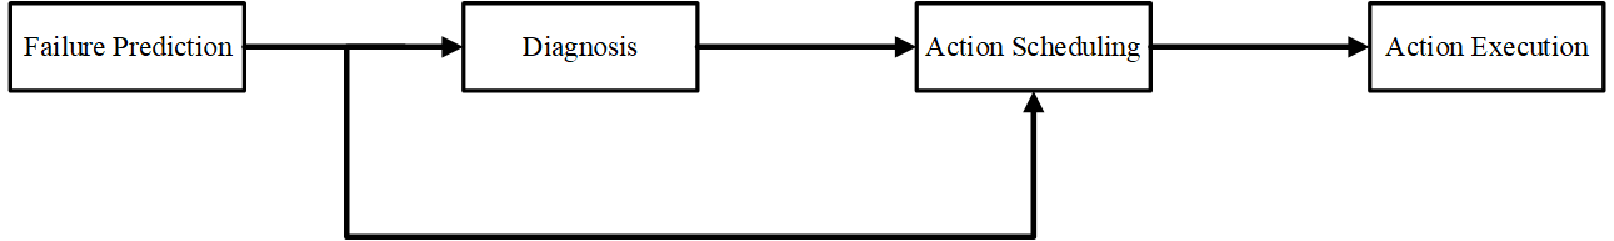
\includegraphics[width=1.0\textwidth]{images/failure_steps.pdf}
    \captionsetup{justification=centering}
    \caption[Workflow support for failure management]{Workflow support for failure management
                                                     (Salfner, Lenk and Malek 2010 p. 3 fig. 2)}
    \label{fig:failure-steps}
\end{figure}

The Figure 1 shows the steps involved in failure management, once a failure event has been predicted,
the prediction should be accompanied with a diagnosis in order to find out the root of the problem
that will cause further upcoming failure events, the role of the diagnosis is to allow the selection
of the right decision when it comes solving the problem using the right method and scheduling the
execution of the task (Salfner, Lenk and Malek 2010).

\section{Root Causes, Faults, Errors and Failures}

According to Wu and Buyya (2015), there is a lot of statistical research that shows the relevance of the human factor
in both planned and unplanned downtime, as it can be seen in the Figure 2, it is a reasonable root cause for the
computer systems failure or downtime, for the unplanned downtime the human error factor represents 15\%
of all unplanned downtime and for the planned downtime which represents 30\% of all downtime events in data
centres there is also a certain percentage of human error that will trigger the computer systems failures,
if the planned downtime would be eliminated, then the percentage of human error factor will increase to a value
of 18\% (see Figure 3). As it can be seen in the figure 2, the majority of faults or failures are caused in
large part by the software element, comparing to the hardware element, but nevertheless, the hardware element
representing 10\% of all computer systems failures or downtime events cannot be overlooked as this number it
will have a significant impact of the runtime of computer systems if failure predictions are provided based
on the hardware element.

\newpage

\begin{figure}[h]
    \centering
    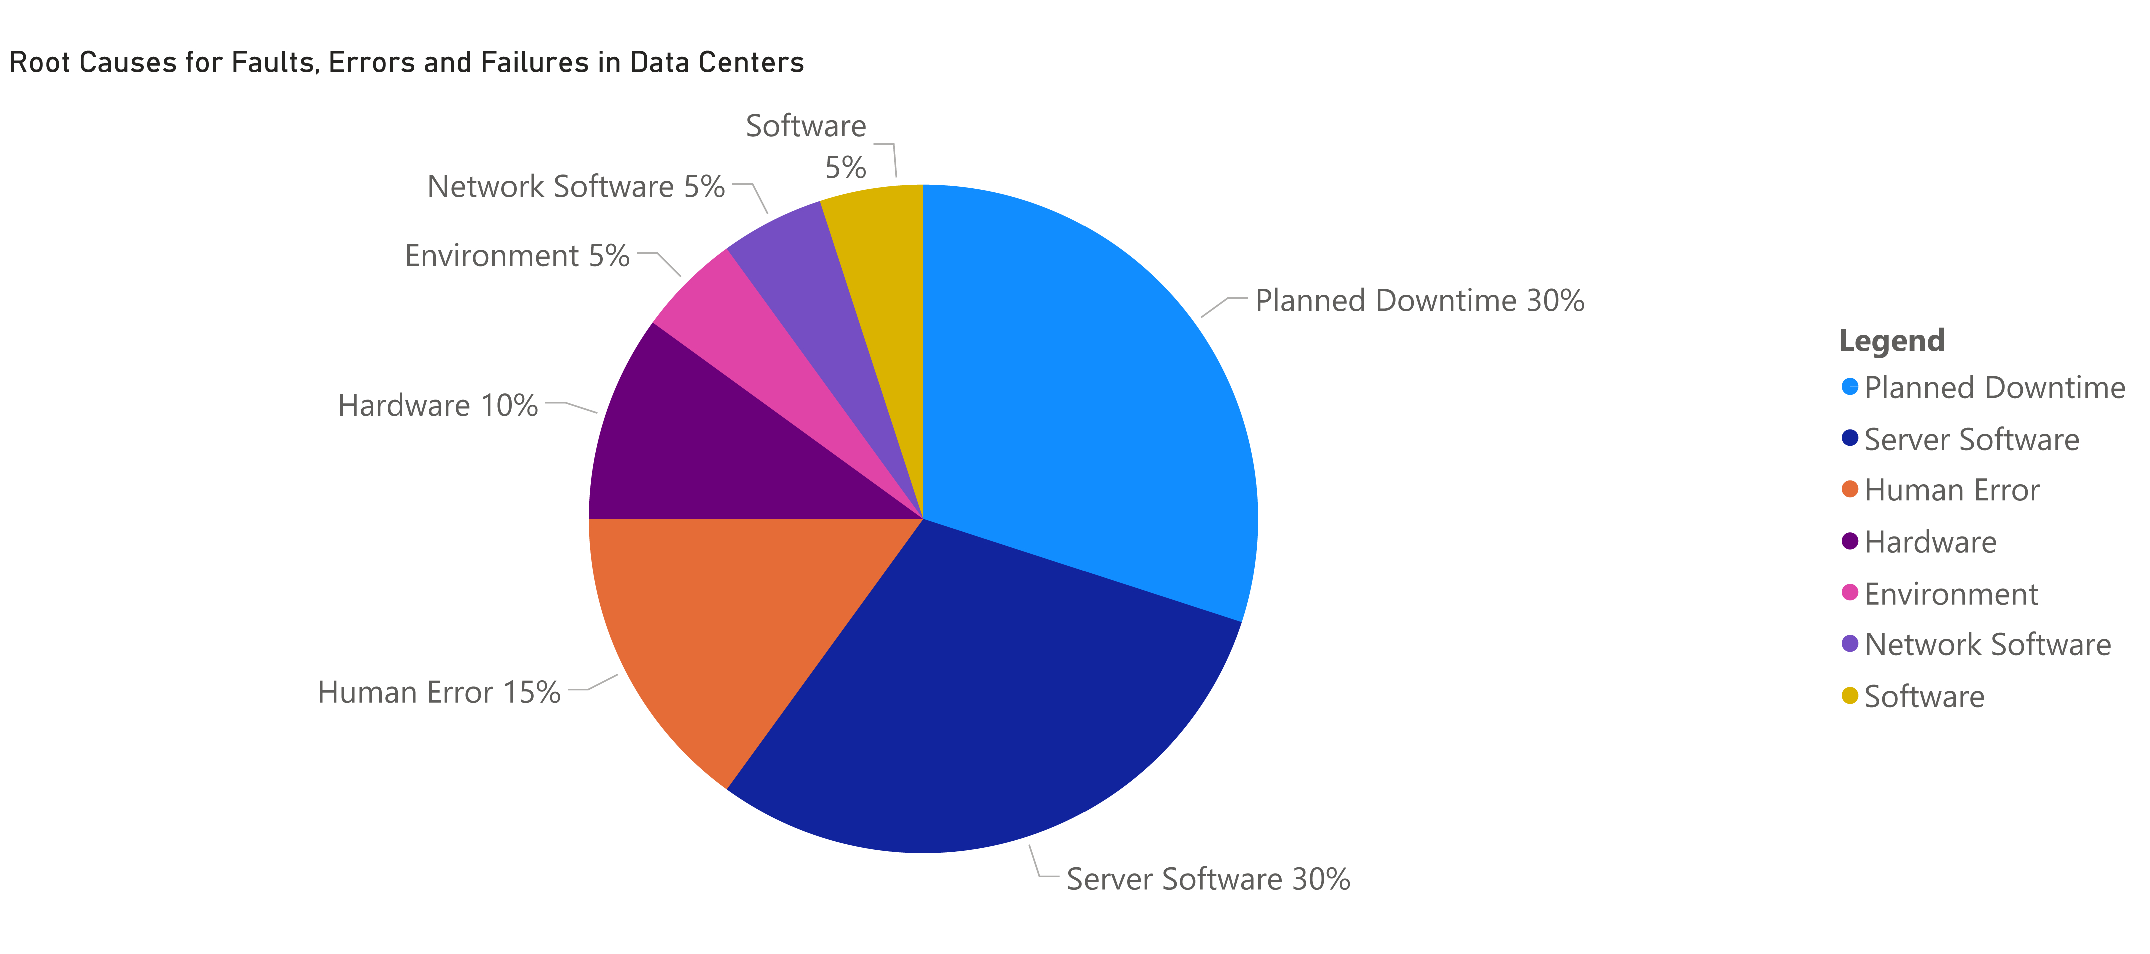
\includegraphics[width=\textwidth]{images/downtime.pdf}
    \captionsetup{justification=centering}
    \caption[Errors, faults and failures in data centres]{Errors, faults and failures in data centres
    (Wu and Buyya 2015 p. 360 fig. 10.8)}
    \label{fig:downtime-events}
\end{figure}

In critical applications, the human error play an important role when talking about computer systems failure or
downtime events, as the human error increases to a more substantial level for critical applications, this
substantial level has the potential to reach a value of 40\% from the operation errors and system outages,
these two elements making 55\% and respectively 22\% of all critical applications failure events or downtime
events (Wu and Buyya 2015). The human error factor represents a significant value of 18\% of all computer systems
failure or downtime events in data centres, Wu and Buyya (2015) suggest that the reason for this substantial value
of human error it is caused by the changes represented by the software upgrades, software patches, system
reconfigurations and maintenance events scheduled for the data centres. These fundamental elements cannot be
banned for a computer system or even more important for a data centre for security reasons and also because
changes are inevitable, an insight into other elements must be performed in order to provide solutions to the
computer systems failure problem, these elements being the hardware element and the networking transmission element,
they are not as predispose to changes as the other mentioned elements and because of this they are good candidates
for computer systems failure predictions.

\begin{figure}[h]
    \centering
    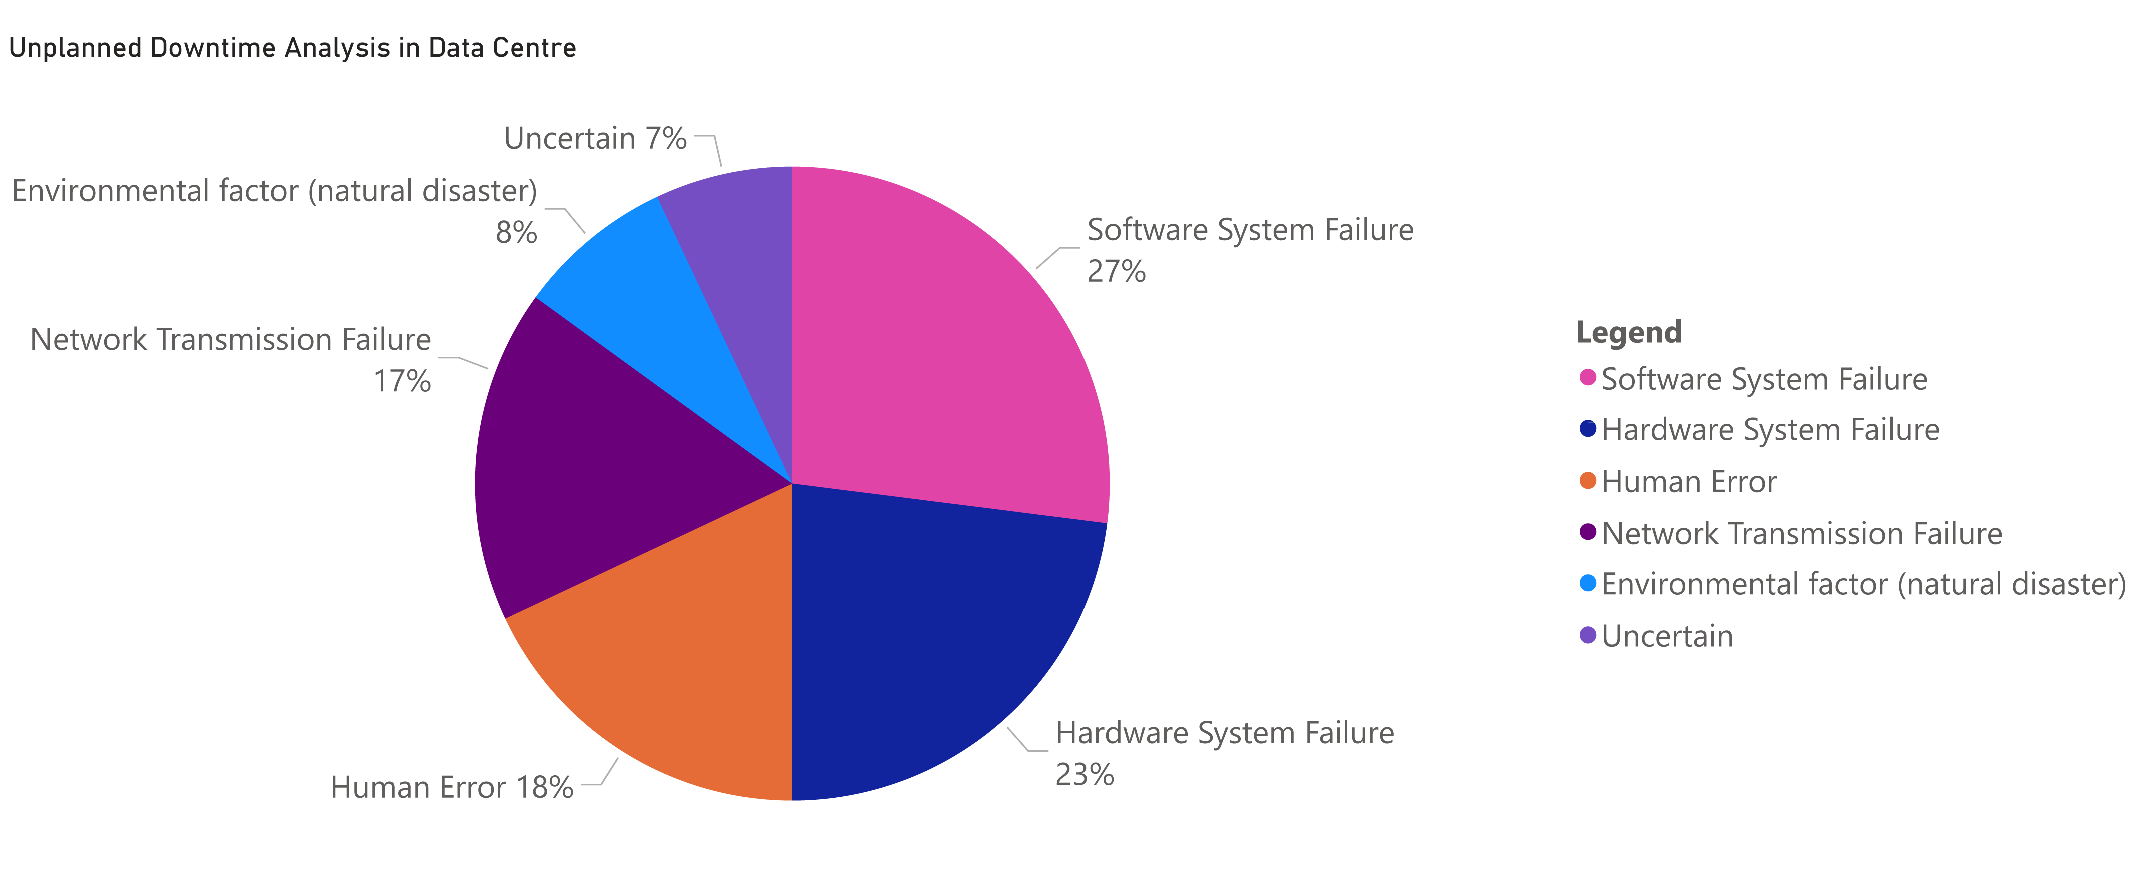
\includegraphics[width=\textwidth]{images/unplanned-downtime.pdf}
    \captionsetup{justification=centering}
    \caption[Unplanned downtime in data centres]{Unplanned downtime in data centres
    (Wu and Buyya 2015 p. 361 fig. 10.9)}
    \label{fig:unplanned-downtime}
\end{figure}

\begin{figure}[h]
    \centering
    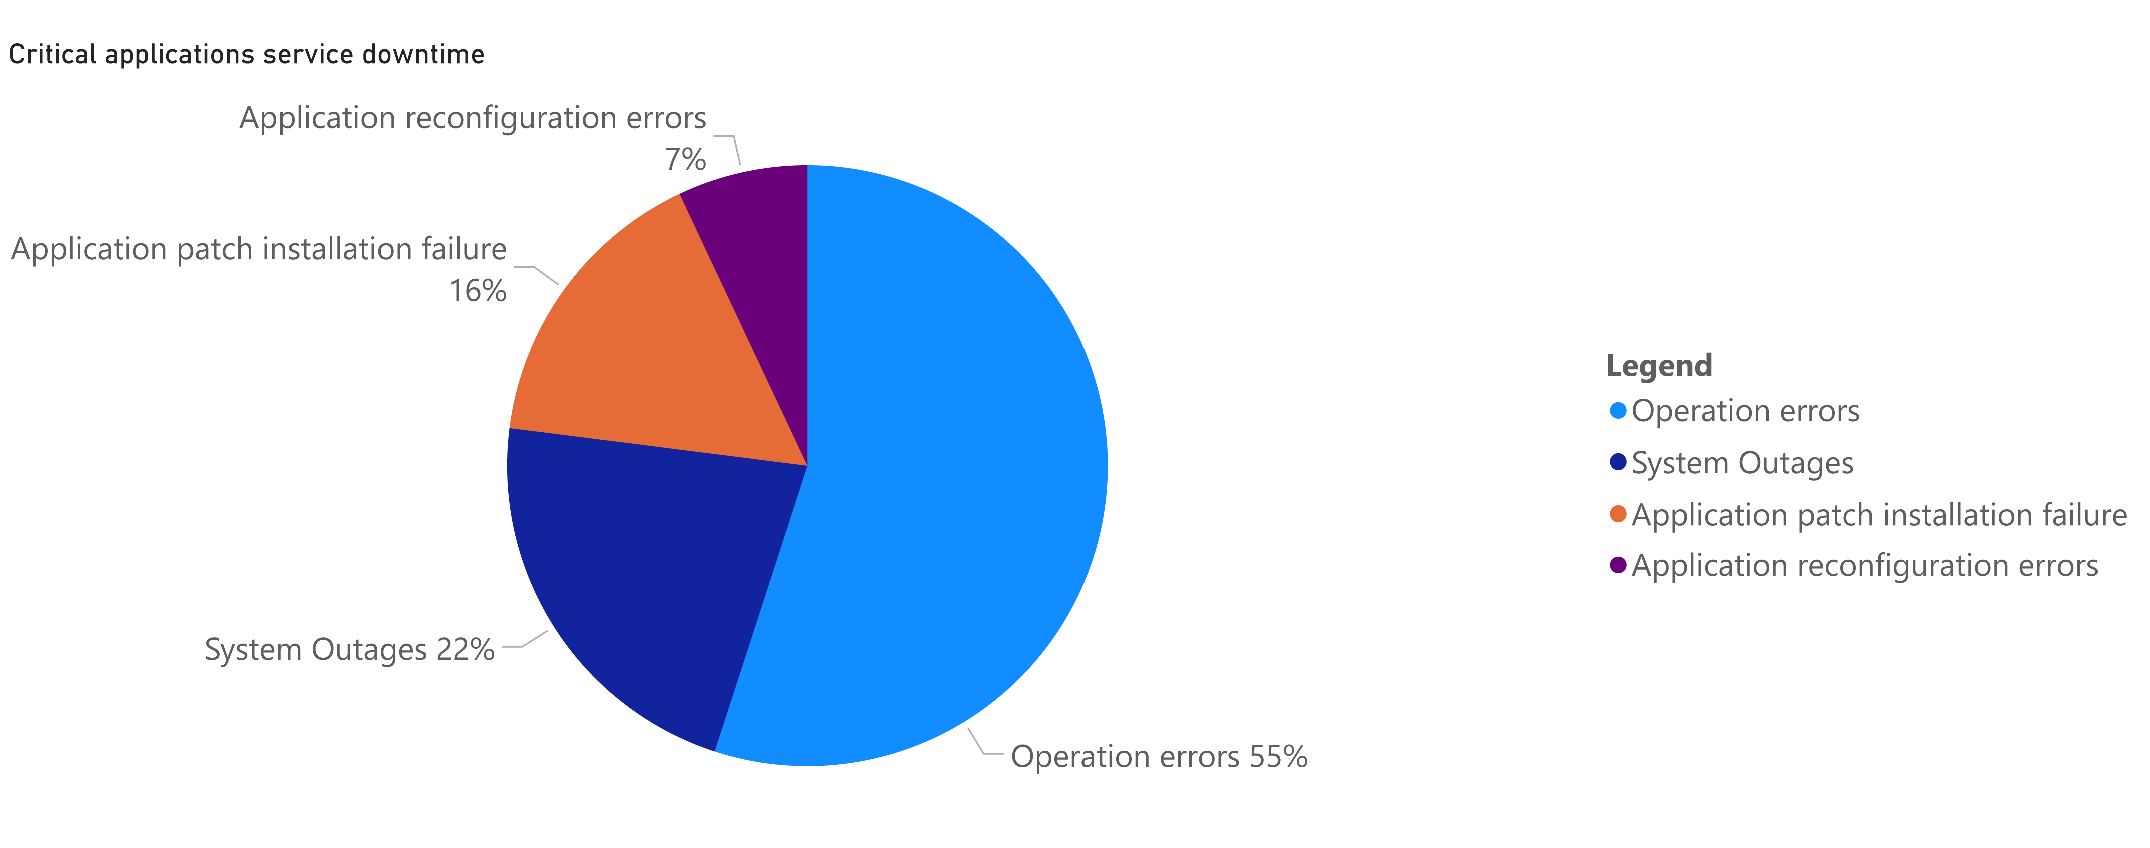
\includegraphics[width=\textwidth]{images/critical-applications-service-downtime.pdf}
    \captionsetup{justification=centering}
    \caption[Critical applications service downtime]{Critical applications service downtime
    (Wu and Buyya 2015 p. 361 fig. 10.10)}
    \label{fig:critical-applications}
\end{figure}

\clearpage

\section{Opportunities and Motivations}

The computing elements and their general influence over data centres mentioned in the Root causes, Faults, Errors and
Failures section naturally bring into discussion the term “Maintenance of Computer Systems”, as this term becomes
relevant for enterprises, institutions, organisations and individuals that need to monitor the performance and state
of their computer systems in order to prevent, mitigate and evaluate the impact of events such as slow response of
the computer systems, the computer systems not responding when specific operations are performed or worst the
failure of the systems which would result in the transition of the system from a working state to a non-working
state accompanied with the loss of essential data. According to Baldoni, Montanari and Rizzuto (2014) a few years
ago the use of proprietary systems provided by a single vendor was a convenient and preferred approach for specific
safety-critical systems related to sectors such as air traffic control, railway control, commercial aircraft and
nuclear power. In addition to those said before by Baldoni, Montanari and Rizzuto (2014), according to Sipos, Moerchen,
Fradkin and Wang (2014) failure predictions can also be used in medical institutions where the medical equipment
it is the core element in the failure predictions process, the logs provided from the medical equipment are
retrieved and used in the maintenance prediction process. Beside the use cases mentioned above, the individuals
that may be concerned about the computer systems failure predictions or downtime events predictions would be
professionals working as computer technicians or systems administrators which are usually assigned with tasks of
ensuring the normal functionality of specific computer systems it is present. The professionals working as
technicians or system administrators would benefit the most from this type of desktop application, as the time
invested into the investigation of hardware or software technical problems could be reduced or even eliminated
by providing near real-time information about the state of one or more monitored computer systems and the
prevention of events that may require maintenance such as the failure of the computer systems which could
vary from the event of a non-responding machine to the transition of the machine from a working state to a
non-working state could be possible if a prediction of hardware or software technical problems is provided
based on past data collected from the computer systems. As it was mentioned before in the Root causes,
faults errors and failure section it is safe to say that data centres, medical institutions, air traffic
controls, railways controls and power plants will benefit the most from computer systems failure predictions
because these kind of predictions will allow the minimization of computer systems failure impact on each of
the entities mentioned if the right measures are put in place before it happens. The applications, services
and resources of a desktop or even server type of computer systems could be organized and scheduled in
a manner which would reduce the impact of the system’s failure whenever predicted by making use of right
techniques which would fit the equipment in cause and classify specific events that would occur in computer
systems as events that would require maintenance or just as informative events if the severity of the events
is low in order to secure the normal functionality of the machines.

\section{Maintenance Solutions}

According to Bastos, Lopes and Pires (2014) in an industrial environment where equipment availability it is
a vital factor in order to ensure the productivity of organisations, the maintenance activities are performed
in order to reduce or eliminate the failures of specific equipment or machinery and with this creating
favourable conditions and allow an increase of productivity for the business or organisation in cause.
The satisfaction of businesses or organisations usually implies the increase of pressure in maintenance systems,
the maintenance process even being considered not to add any value to the businesses or organisations,
but nevertheless the maintenance process it is an important factor that will contribute to the reduction of
business or organisation costs and allowing the equipment to function in normal conditions. The main factor
of acknowledgment related to computer systems or technological systems failure are some indicators that will
proceed such failure events in 99\% of the maintenance events cases. The breakdown maintenance or runtime
failure also called as the unplanned maintenance event it is the earliest maintenance technique which takes
place at the breakdown event of the machine in cause, the later technique it is a preventive technique which
will allow a time interval to take actions also called as planned maintenance (Bastos, Lopes and Pires 2014).
The problem of maintenance of computer systems or technological systems presents both commercial and open
source solutions, these solutions can be categorised as reactive maintenance solutions and predictive
maintenance solutions. The reactive maintenance solutions can be defined as a mechanism that can be used to
respond to technical problems that have occurred in computer systems or technological systems at a specific
point in time where no time interval has been provided by the solution in cause in order to take any measures
that could be used to mitigate the impact of the technical problems that have occurred in the system in cause,
it is safe to say that a reactive maintenance solution will allow a response to the maintenance events after
the impact has been felt by the computer system or technological system in cause. The predictive maintenance
solutions can be defined as a mechanism that will allow the provision of an informative event related to a
possible technical problem that is likely to occur in the near future in a computer system or technological
system accompanied with a diagnostic that will contain the root cause of the technical problem and time
interval where actions can be performed in order to mitigate the impact of the maintenance problem
(Bastos, Lopes and Pires 2014).

\newpage

\section{Challenges and Impediments}

According to Salfner, Lenk and Malek (2010) the core elements that contribute to the challenges and impediments
of computer systems failure or downtime events are the dependability and resilience factors. These factors are
represented by the continuous increasing of computer systems complexity, the continuous increasing of cyber
security problems such as attacks and threats, the continuous increase of connectivity and interoperability
of technological systems, the increasing use of third party and open source software and last but not the
least the dynamic and unforeseen runtime of computer systems. The dynamicity of computer systems can be
reflected by the frequent system configurations, system reconfigurations, software updates and hardware upgrades.
The elements that contribute to the difficulty of computer systems failure predictions mentioned by Salfner, Lenk
and Malek (2010) are not the only factors that will increase the difficulty of failure predictions when talking
about computer systems or any technological systems. In order to provide maintenance predictions signals for a
technological system, an insight must be taken into the running state of the technological system or equipment
in cause, this insight it is performed either by making use of the existing hardware sensors present on the
components of the technological system or the equipment in cause or additional hardware sensors will be added
to the technological system’s components or equipment in order to allow the recording and retrieving information
such as temperature signals, voltage and other information of interest, once the hardware sensors have been put
in place or they already exist on the technological system or equipment, the failure or maintenance predictions
module can then send alerts or signals of possible events that will inform the control centre of any components
values deviating from normal parameters, these deviations of values are an important factor in predictive
maintenance as this deviations of values could result in the failure of the technological system or equipment
in cause (Sipos, Moerchen, Fradkin and Wang 2014). A more technical approach and confirming the continuous
increasing of computer systems mentioned above  there are other elements that will increase the difficulty of
computer systems failure predictions, according to Botezatu, Giurgiu, Bogojeska and Wiesmann (2016) when
adventuring into computer system failure predictions a known fact is that all computer systems will present
a storage system, this system being an important component and also the root cause of the most computer system
failures in data centres, in most cases this storage system it is a hard disk and usually all hard disks present
a mechanism called Self-Monitoring, Analysis and Reporting Technology (S.M.A.R.T), this mechanism will contribute
to the difficulty of trying to predict unforeseen failure events based on the storage system. The dynamicity of
the hard-disk S.M.A.R.T indicators will be the main factor of difficulty as these indicators are manufacturer
specific, the specialised encoding of the hard disk indicators will be different for each hard-disk model and
their normalization values will also vary depending on the manufacturers.

\newpage

\section{Hardware Sensors}

The hardware sensors in computer systems or technological systems have the role to measure the physical behaviour
of specific components that the machines or technological systems present in their composition, these computer
systems or technological systems usually are executing cyber space but this is not a requirement for the hardware
sensors in order to be present on the components of the computer systems or technological systems in cause.
In addition to the physical behaviour measuring or monitoring of the components, the hardware sensors also
sample the physical effects of the processes that allow the transfer and processing of information.
The hardware sensors can monitor or measure the behaviour of computer systems components from the internal
input and output channels to the LED status of the lights and for this reason the hardware sensors are an
important element when trying to make predictions related to computer systems failures or downtime events
(Edgar and Manz 2017).

\subsection{Processor}

The \acrfull{cpu} sometimes referred as the Central Processor or simply just as Processor it is
a hardware component which can be considered the brain of a computer system, this component it is considered
the brain of a computer system because it is the place where the most calculations take place in a computer system.
The Processor has the role to execute the instructions of a computer program which are retrieved from the memory
of the computer system in cause and because of this in terms of computing power it can be considered the most
important piece of hardware in a computer system (Beal 2020). According to Bach (2014) it is a known fact that
modern computer systems processors present some mechanism of active cooling in order to ensure their normal
functionality without producing a runtime failure but there is a little official information on how the modern
processors are affected by different temperatures when it comes to their performance. When it comes to older
computer systems processors the behaviour presented by this chips when encountering high temperatures would be
a failure of \acrfull{cpu} which will result in the transition of the working machine to a
non-working machine caused by the overheat of the processor component, the modern computer systems on the other
hand have the capability to adjust their frequency according to the temperature they are functioning at in order
to prevent the failure of the technological system in cause, this prevention of failure has the drawback of a
decrease in the performance for the processor in cause as the temperature increases the processor will try to
protect itself and slowing performance (Bach 2014). The \acrfull{cpus} or Processors are not excluded
from the zone of possible failure, the processors can fail if the conditions of failure are present but most
processors are one of the most reliable components in a technological system or workstations as \acrfull{cpus}
have a small overall failure rate of just 0.2\%, this will result in a single processor failing in
500 of processors when the components are of production process and delivered to the customers (Bach 2014).
It is safe to say that using the temperature sensors of the processor component will not present a good candidate
for failure predictions but it may present a good candidate for anomaly detection.

\newpage

\subsection{Memory}

The computer systems memory it is a term used to represent multiple types of data storage technologies that computer
systems can use, these types of memories are the \acrfull{ram}, the \acrfull{rom} and Flash
Memory (Rubens 2019). The computer systems present many types of memory, the most common distinction is between
primary memory and secondary memory, the latter one being more commonly known as storage memory. The primary
memory includes the \acrfull{rom} and \acrfull{ram} and it is located close to the \acrfull{cpu} or
Processor on the computer motherboard, allowing the Processor to read data from the
primary memory in a relatively fast manner, in other words the primary memory has the role to store data that
the \acrfull{cpu} will need to have access as soon as possible and not being required to wait
for delivery of data. The secondary memory most commonly it is usually physically located in a separate storage
device, for example a \acrfull{hdd} or a \acrfull{ssd}, the secondary memory in cause being
connected to the computer system in a direct way via a \acrfull{sata} cable or
over a network (Rubens 2019). The \acrfull{ram} as the name implies it has the role to store data
that can be accessed in a random manner, this type of memory it is fast to read and write which makes it a
volatile type of memory. The Read-Only Memory as the name implies it has role to allow data to be read from
this type of memory and no data can normally be written to it. According to Bach (2019)  the \acrfull{ram}
used to be one of the most reliable pieces of hardware but in the last 5 years it has improved
even more, the \acrfull{ram} has an overall failure rate of 0.41\%, this value will result in a
single Random Access Memory will fail out of 244 of \acrfull{ram} hardware components, but the
failure rate presented on the customers side or the field failure rate had a value of 0.07\%, this value
representing a single failure out of 1400 of \acrfull{ram} sticks once the components are
presented in the customers possession. It is safe to say that using the sensors of the \acrfull{ram}
component will not present a good candidate for failure predictions but it may present a good candidate
for anomaly detection when considering the voltage as the main factor of analysis.

\newpage

\subsection{Storage System}

Data storage can be represented by the collective methods and technologies that allow the capture and retainment
of digital information on entities such as electromagnetic, silicon and optical storage media. The word storage
is used most of the time to represent the devices connect to a computer system, the connection being made through
input and output operations, these includes Hard-Disks, flash media and other media entities. These days the main
types of storage media are the Hard-Disk Drives, Solid-State Drives and optical storage, the Hard-Disk
Drives are widely used to store data in computer systems used as personal computer, servers and enterprise storage
systems but the Solid-State Drives are also start to present an increase in the use for similar purposes (Rouse 2018).
According to Botezatu, Giurgiu, Bogojeska and Wiesmann (2016) the costs caused by computer systems failures or
downtime events have increased in a significant way in the past years for data centres, these costs are ranging
from the minimum cost of \$5,600 per minute in 2010 to the maximum cost of \$8,851 per minute in 2016. The failure
of technological equipment it is the most important factor that contributes to the downtime events. The Hard-Disks
Drives are one of the most frequent components to fail in a computer system or in information technology environments.
The reliability and performance of the Hard-Disk Drives are affected especially by factors such as duty cycles,
workloads and temperature, the reliability problems are the most important as the severity of these problems will
cause the failures of the hard-disk drives and eventually the need to replace the hard-disks in cause. Hard-Disk
Drives failures can be categorised as either predictable failures or unpredictable failures, the unpredictable
failures are represented mostly by the electronic components of the hard-disk in cause not being functional anymore,
this event being sudden without any warning of possible crashes and because of this the unpredictable failures
caused by the electronic components cannot be predicted by monitoring. The predictable failures on the other hand can
result from slow processes represented by normal usage of the component that usually progresses over time, most of
the time over month or years. The latter one will allow the analysis of possible predictive failures. The hard-disk
drive sensors or the \acrfull{smart} system can be used to monitor the
factors that will cause the failure of the hard-disk or when a failure is most likely to occur. Most of the time
manufacturers implement a system that makes use of these S.M.A.R.T attributes in order to provide predictions of
possible failures for the hard-disks, but these embedded models are not very efficient as they present minimal
considerations of the technical problems that could occur and for this reason are considered simple models that
cannot offer an insight about the unforeseen failure events due to the threshold-based normalisation, the focus of
the design being on avoiding false alarms of possible failures. According to Klein (2020) Blackblaze was in the
possession of 150,757 hard drives used to store customers data, as of 30 September 2020 an evaluation of the
reliability of these hard-disks was performed, this evaluation resulted in an overall or annual failure rate
of 0.89\% for all hard-disk drives. It is safe to say that using the sensors of the Hard-Disk Drives
component or the S.M.A.R.T indicators will present a good candidate for failure predictions as it is a component
that is frequently causing computer systems or technological systems to fail and it has the necessary attributes
in order to make the predictive alerts happen.

\section{Software Implications}

The manufacturing companies depend generally on the reliability of the products that are being produced by the
companies in cause in order to have success and to ensure their existence. This dependability that the manufacturing
companies present for the reliability of products in cause brings into discussion the scheduled maintenance of
equipment that companies are using, this scheduled maintenance it is a necessity for this kind of companies in
order to ensure the normal functionality and the avoidance of possible failures of any kind of technological
systems or equipment, the scheduled maintenance in this case it is used as a safeguard. The maintenance it is
performed separately most of the time for all components, the selection being made on usage, performance or
simply because of fixed scheduled maintenance, just like any other activity performed within a manufacturing
company and not only, the scheduled maintenance are not free of cost, the scheduled maintenance it is labour
intensive, not free of cost and not efficient when it comes to identifying technical problems that develop
between technicians visits. Unpredictable failures of computer systems or technological systems will still
occur despite technicians’ visits, on the other hand, the predictable failures or prediction of maintenance
events related to computer systems or technological systems can determine the condition of the system in cause
and allow the repair or the evaluation that must be performed. The ultimate goal of the predictive maintenance
or the predictive failure for the technological systems in cause is to allow pro-active scheduling and corrective
activities that will result in solving the problems created by unexpected failure of the systems in cause. Modern
technological systems or information technology equipment is most of the time operated with the help of software
applications, for example in the case of medical equipment, most operations such as warnings related to scan
performed on a patient can be retrieved and used to created medical reports and to perform specific calibrations,
these activities are controlled by a software application. The software applications most of the time are producing
some king of logs to represent their operations, these logs are exist in order to inform the user of the software
application about the activities that are being performed at a specific point in time by the application in cause
or to reflect the software developers instructions or ideas about what valuable information must be mentioned, for
example error messages, internal states or exceptions. The information found in the logs provided by the software
applications can be used to trace back how a piece of hardware was used and to have an insight about the functionality
of the component in cause by analysing the content of the logs for any errors or internal state abnormalities. However,
the use of information related to technological systems or equipment found in log files can present many challenges and
impediments when it comes to failure predictions as it has not yet been fully explored and understood since logs of
software applications are used for debugging purposes they contain minimal information that can be used for failure
predictions when it  comes to technological systems or equipment, beside the minimal information the logs files also
need data pre-processing actions as the logs contain symbols, categorial variables, times series and characters which
are not structured, the data also being considerably large which will lead to time consuming analysis due to the
calculation power required (Sipos, Moerchen, Fradkin and Wang 2014).

\section{Computer Network Architectures}

Having Access to networks or to the internet especially is becoming a fundamental element and most of the time a
requirement for software applications as applications frequently need some kind of internet access in order to
provide services to the users. The \acrfull{iot} allows more and more devices to be interconnected and
because of this understanding how to have access to networks becomes a crucial element (Reese 2015).
The term Computer Network Architecture refers to the physical and logical design of computing elements such as
hardware, software, network protocols and media when it comes to transmission or transfer of data, in other words
this term can be defined as a method that represents how computers are organised and how tasks are allocated to
the computers. (JavaTPoint 2018). A computer network it is composed of nodes and links which are combined in order
to create a network architecture. A device connected to the \acrfull{iot} it is usually called a node
and a computer node is usually called host, the communications between these nodes are done by making use of
protocols such as HTTP, TCP and UDP. The network nodes can include devices such as \acrfull{nic},
bridges, switches, routers and hubs, these elements are all involved in the transmission of data between computer
systems and other interconnected technological systems. The network links can be represented by the wires such as
coaxial cables, twisted pairs, fibre optics and wireless such as Wi-Fi or satellite communications, these links
can support a range of bandwidth and address specific communication needs. (Reese 2015). The communication between
the network nodes it is done by sending a message across the internet from a home computer or any computer system,
once this event happens, the computer’s unique address is not globally unique and for this reason any messages sent
between the network nodes or the computer systems will by handled by the \acrfull{nat} device
which will allow the changes of the address to an address that can be used for the \acrfull{iot} or
simply the Internet and allow a single IP address to be used for multiple nodes on the network. There are two
types of computer network architectures, these are the \acrfull{p2p} architecture and the \acrfull{cs}
architecture (JavaTPoint 2018).

\begin{figure}[h]
    \centering
    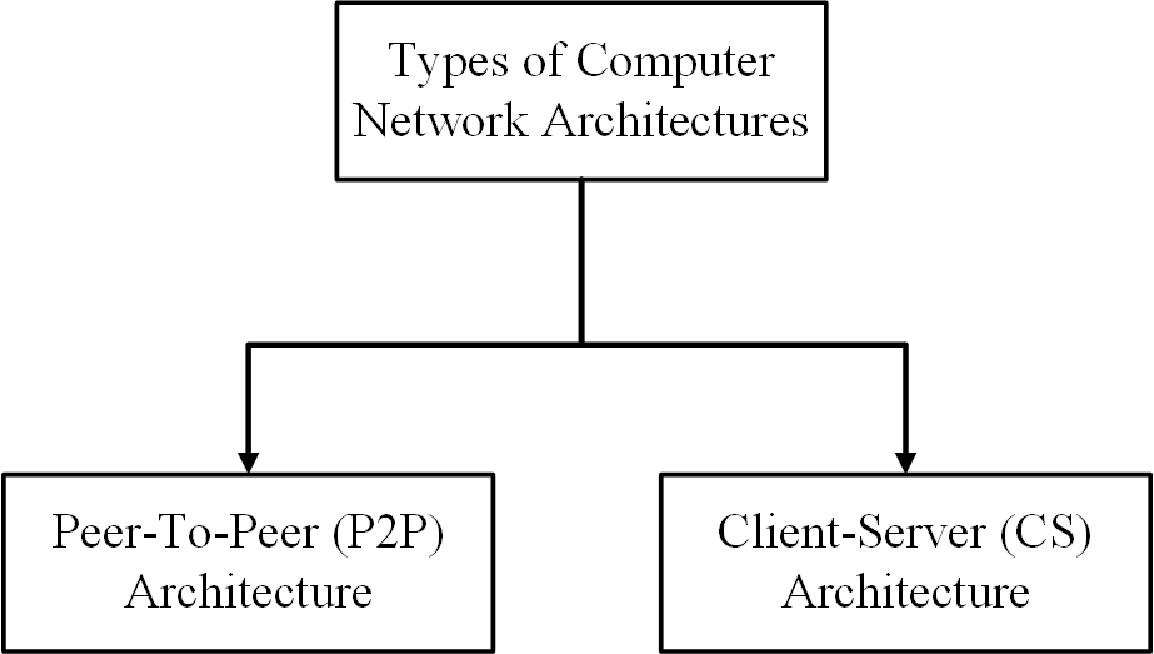
\includegraphics[width=0.65\textwidth]{images/network-architectures.pdf}
    \captionsetup{justification=centering}
    \caption[Computer Network Architectures]{Computer Network Architectures (JavaTPoint 2018 fig. 1)}
    \label{fig:network-architectures}
\end{figure}

\subsection{Data Transfer using Peer-to-Peer Architecture}

The Peer-To-Peer (P2P) network can be defined as a network where all the nodes or computer systems are linked
together and all nodes are both clients and servers at the same time with equal privileges and responsibilities
when it comes to the transfer and the process of data (Neagu 2019).

\begin{figure}[h]
    \centering
    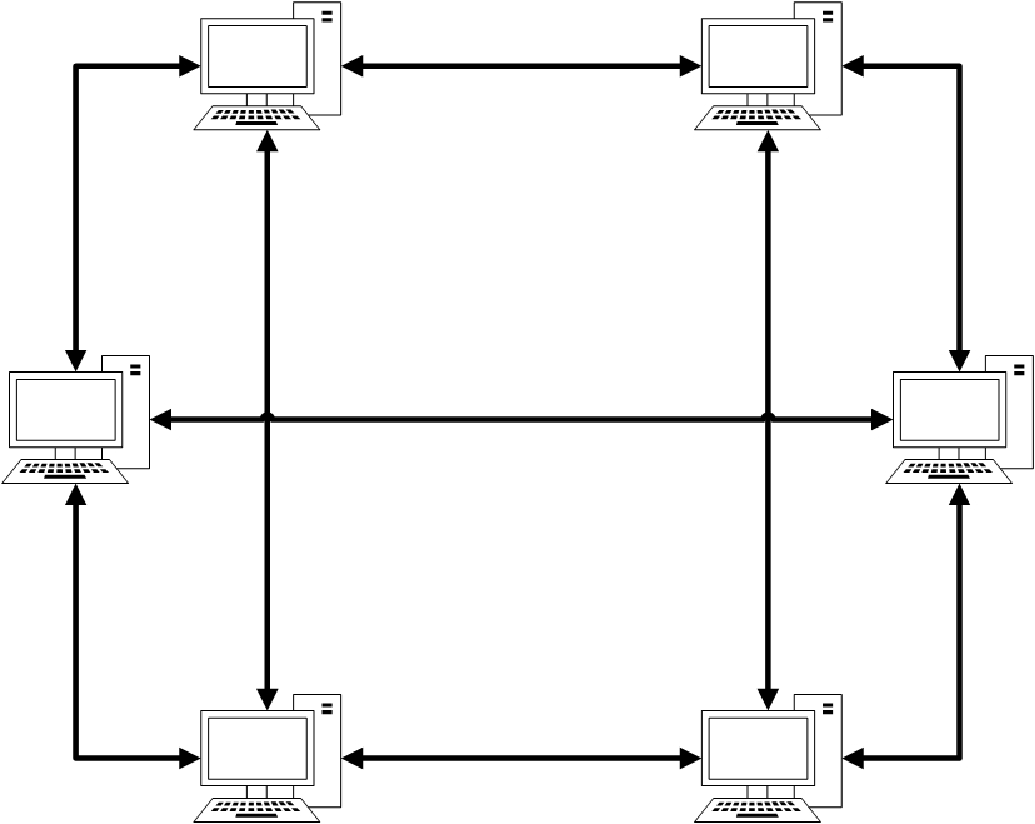
\includegraphics[width=0.55\textwidth]{images/peer-to-peer.pdf}
    \captionsetup{justification=centering}
    \caption[Computer Systems Peer-To-Peer (P2P) Simulation]{Computer Systems Peer-To-Peer (P2P)
                                                             Simulation (Neagu 2019 fig. 1)}
    \label{fig:network-peer-to-peer}
\end{figure}

\subsection{Data Transfer using Client-Server Architecture}

The Client-Server (CS) network can be defined as a network where the nodes or computer systems are linked together
to a centralised system called server, the nodes can be called clients which can access resources from the
centralised system or server as the privileges and responsibilities when it comes to the transfer and the
process of data are not equal, the server having more privileges and responsibilities (JavaTPoint 2018).

\begin{figure}[h]
    \centering
    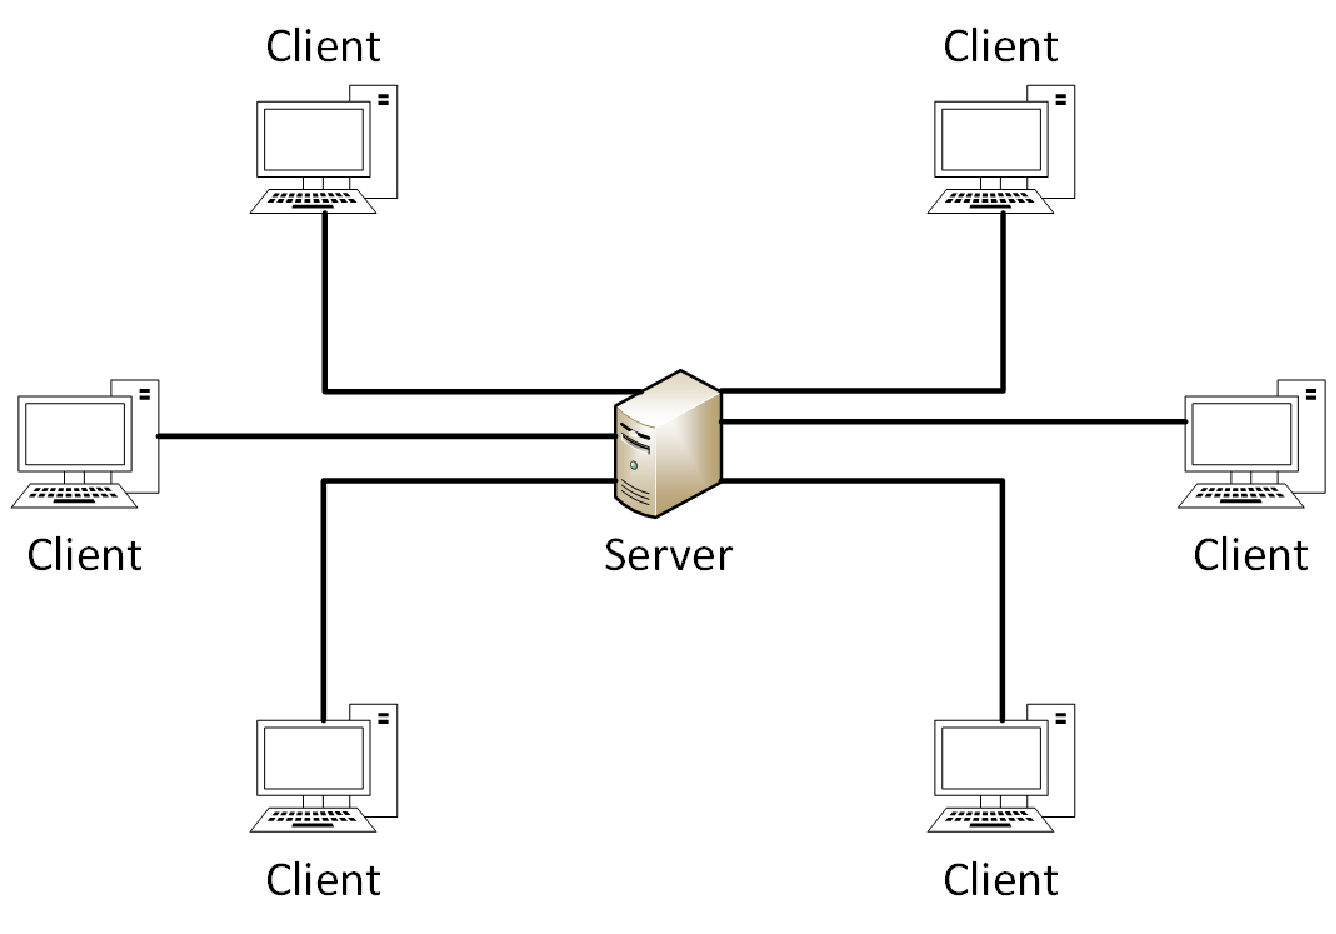
\includegraphics[width=0.55\textwidth]{images/client-server.pdf}
    \captionsetup{justification=centering}
    \caption[Computer Systems Client-Server (CS) Simulation]{Computer Systems Client-Server (CS) Simulation
                                                             (JavaTPoint 2018 fig. 2)}
    \label{fig:network-client-server}
\end{figure}

\section{Approaches and Techniques}

Numerous approaches have been performed in order to provide a solution to the maintenance of computer systems problem.
Some of the most common approaches would be the ones that make use of machine learning techniques such as
classification and regression models in order to analyse system log files which could contain data from simple
system log in information to more relevant information when it comes to maintaining a machine such as software
failure or hardware failure.  Fulp, Fink and Haack (2008) suggest that the prediction models that have been used
for the maintenance or failure of computer systems problem would be some of the standard machine learning models
such as the Bayes Networks Model, the Hidden Markov Model and Partially Observable Markov Decision Process,
these models have been used in association with an analysis of operating systems events logged and stored on
the computer’s hard-disk in order to be able to signal any occurring failure of the system in near real-time
and also make predictions based on past data. In addition to those said, He, Feng, Lee, Wang, Han and Liu (2020)
suggest that some of the most common approaches to the maintenance or failure predictions of computer systems
are the use of the binary classification models such as Support Vector Machines and Linear Logistic Regression.
Analysing the state of the storage component of the computer system in order to identify any decrease in the
response time or failure of the machine is another approach undertaken in order to identify any maintenance
event for a system based on storage component state, the storage system being a hard-disk in most cases as
Botezatu, Giurgiu, Bogojeska and Wiesmann (2016) indicate, the hard-disk state, response time and utilization
are the main factors that have been used when making use of machine learning models. In addition to those said
about the hard-disk element, He, Feng, Lee, Wang, Han and Liu (2020) suggest that in order to provide a solution
to the failure of computer systems based on the hard-disk component, the binary classification machine learning
models must use the information found from the labels that enhance the accuracy of disk failure prediction based
on S.M.A.R.T indicators which can be translated to features in a dataset. The failure or maintenance time prediction
machine learning algorithms based on the use of information found in the S.M.A.R.T system make a good use of the
systematic or gradual changes in these indicators, though these techniques are unable to handle well data containing
a lot of noise or if the dataset it is imbalanced. Computer systems or technological systems log files are a vital
factor when trying to offer a history or an audit of both hardware and software events. The hardware and software
events in this context refer to information such as simple log in information to failure of applications and
hardware components. Analysing system log files it is a good and efficient approach when considering failure
predictions as it is possible to make use of some information found in the log files if the right features are
extracted. Most of the time log files are text files which contain messages that are usually sent by software
applications indicating the operations performed. Software applications can store information in the log files
with the help of the syslog process which allows this process to happen. Many types of log files exist, yet the
most interesting ones are those that contain S.M.A.R.T messages, these messages providing information about the
health and status of the hard-disk drive component of a computer system (Fulp, Fink and Haack 2008).

\subsection{Failure Predictions using Support Vector Machines (SVMs)}

The machine learning algorithm called Support Vector Machines (SVM) it is a supervised machine learning method
that is used as a binary classification algorithm, the binary classification meaning a class label it is
required in order to perform the training of the model. When a dataset is given to the machine learning
algorithm called Support Vector Machines (SVM) for the training, the dataset must contain a class label,
if this requirement it is met the algorithm will try to separate the binary elements into a classification
view using a plane that separates the two classes. The algorithm will attempt to separate the two classes
mentioned in the dataset, if this operation is not possible, meaning the two classes cannot be separated
linearly, then it is possible to use the higher-dimensional space to allow the finding of a separator.
If the two classes can be separated using a linear plane then the Support Vector Machines algorithm can
assign new non label data to a specific class. When it comes to maintenance or failure predictions of
computer systems, the Support Vector Machines (SVM) algorithm can be used by analysing a series of messages
which are or are not associated with a specific failure in the near future. Using the machine learning
algorithm called Support Vector Machines (SVM) associated with information related to S.M.A.R.T indicators
stored in the system log files has achieved a prediction accuracy of 73\% and an error rate of 27\%
(Fulp, Fink and Haack 2008).

\subsection{Failure Predictions using Hidden Markov Model (HMM)}

The Hidden Markov Model (HMM) it is a machine learning algorithm that can be categorised as a statistical
model which has the role to create relationships between variables in the form of mathematical equations
and because of this the system modelled can be considered a Markov process with hidden states, in other
words the Hidden Markov Model (HMM) can be considered the simplest dynamic Bayesian Network. Comparing
to the simple Markov Model, in the Hidden Markov Model (HMM) the system state is not directly visible
to the analyser or observer which leads to the fact that the Hidden Markov Model (HMM) can only have
access to the result or output of the system in cause and not the entire state information.
The Hidden Markov Model (HMM) can be used for assumptions such as a fault can generate a decrease
in the performance of a system which could eventually lead to a complete failure of the system in cause,
this being the approach undertaken in case when using the Hidden Markov Model. The mechanism related to
the maintenance or failure prediction of a technological system implies the monitoring of the distributed
system’s behaviour by trying to find possible anomalies that could lead to failures, the failures usually
being created by faults or errors, once this is done alerts related to software will be provided if the
system state degradation becomes severe. Using the machine learning algorithm called Hidden Markov Model
(HMM) associated with information related to assumptions based on the state of the system has achieved a
prediction precision of 88.51\% and a false positive rate of 11.26\%. (Baldoni, Montanari and Rizzuto 2014).

\section{IT Systems Failure Predictions for Businesses}

\begin{figure}[h]
    \centering
    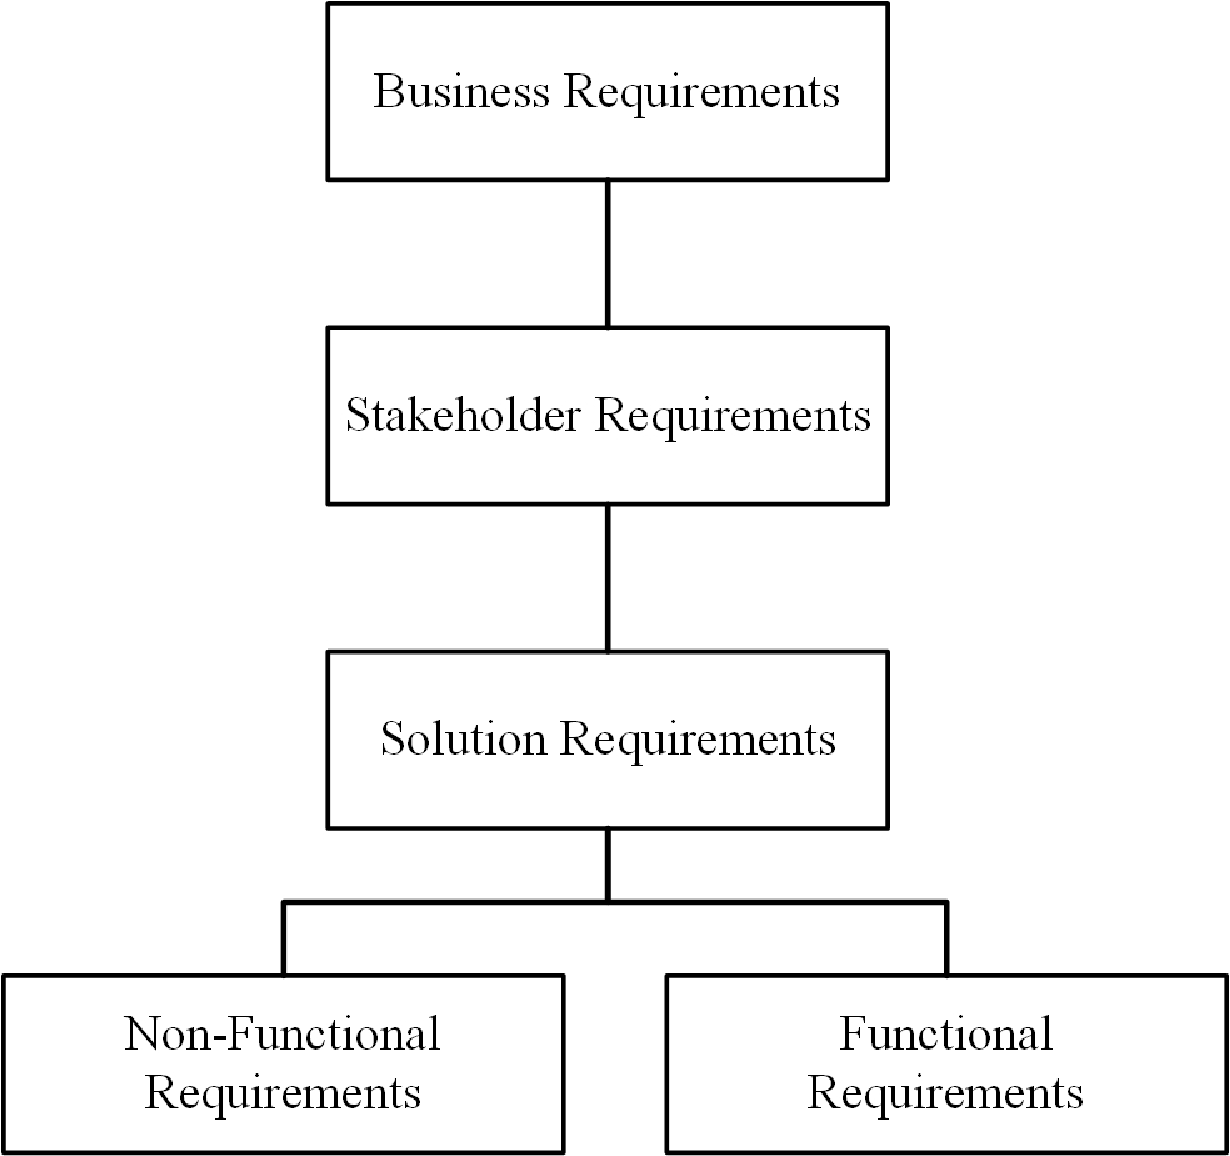
\includegraphics[width=0.45\textwidth]{images/business-requirements.pdf}
    \captionsetup{justification=centering}
    \caption[Workflow support for business needs]{Workflow support for business needs
                                                  (Wu and Buyya 2015 p. 66 fig. 2.12)}
    \label{fig:network-business}
\end{figure}

\subsection{Business Requirements}

The strategic analysis of a business can also be referred as a method that will allow the creation of the business
requirements, these requirements being the result of the analysis performed. As it can be seen in the figure 5,
the business requirements are the top level of the workflow support for the business needs and because of this
the business requirements must be developed as the analysis of business activities are performed.

\subsection{Stakeholder Requirements}

According to Wu and Buyya (2015) the stakeholder requirements depend largely on the stakeholder of the business
as the stakeholder represents all the persons involved in a technological project, while the stakeholder
requirements represent an interface that provides solutions between other stakeholders, the stakeholder
requirements will ensure that all other persons involved in a project as a group will be working towards
the same ultimate goal and because of this the requirements can be considered as a method of consolidation
or anticipation for the high-level business requirements that will allow the creation of comprehensive,
practical, measurable and realistic solution requirements.

\subsection{Solution Requirements}

The solution requirements of a specific business can be referred as the business requirements but in a more
comprehensive manner. They are constituted of two other sub sets of solution requirements; these two sub
sets are the non-functional and functional requirements which will be translated into project tasks
(Wu and Buyya 2015).

\section{Conclusions}

The background chapter has shown the importance of the maintenance actions that must be performed for computer
systems, technological systems and equipment in order to ensure the stability of the systems in cause. In this
chapter it was also discussed why businesses must take into account factors such as the labour investment and
costs which will increase due to inability of the business to understand that the classical reliability theory
related to computer systems or technological systems will not be able offer any solutions to the maintenance
or failure of systems problem which will ultimately lead to the consequences to be felt significantly by the
entities in cause if no measures are put in place to mitigate the failure events. In addition to the importance
of the maintenance events in this chapter it was discussed that the failure predictions must be accompanied
with a diagnostic of the failure root cause in order to be able to anticipate and execute the necessary actions
to allow the system to remain functional and in a stable state. After the root causes, faults and errors were
evaluated it was concluded that the hardware element presents a good candidate for further investigations in
order to accentuate the research towards this area which could lead to a decrease of 10\% of computer systems
failures in data centres, the failure events being represented by the hardware element. Further into the research
it was concluded that the maintenance solutions related to computer system or technological systems can be
categorised as either reactive maintenance solutions or predictive maintenance solutions, the latter one being
the focus of this research. During the extended research of the predictive maintenance solution it was concluded
that providing a solution to computer system failure predictions problem will present many challenges and
impediments due to the continuous increase of technological complexity and the dynamic runtime of computer
systems. After the hardware element was set as the centre of research for failure predictions, the hardware
elements that were investigated for possible failure predictions related to computer systems were the Central
Processing Unit (CPU), the Random-Access Memory (RAM) and the Hard-Disk Drive (HDD) component. It was concluded
that the Hard-Disk Drive it is more predispose to failure than the other components and it presents the best
candidate for failure predictions as it has the suitable attributes that will allow the failure predictions
happen. Once the predispose hardware component to failure has been identified, the software implications have
been investigated and it has been concluded that the certain applications will save relevant information into
system log files which could be beneficial to the process of failure predictions. The final evaluation was the
analysis of possible candidate machine learning algorithms that could solve the problem of technological systems
failure predictions, the Support Vector Machines (SVM) algorithm and the Hidden Markov Model (HMM) were evaluated
and both algorithms present promising results, the Hidden Markov Model having the best results with a precision
rate of 88.51\% in the favour of the Support Vector Machines with a 73\% accuracy. The machine learning algorithm
called Support Vector Machines (SVM) will be used for the implementation of the solution as this algorithm it is
used in association with the S.M.A.R.T indicators which are a core element for the failure predictions process.
\newline
\newline
Research Question: Is it possible to build a solution using the Support Vector Machines (SVM) algorithm for the
maintenance of computer systems problem?



    \chapter{Specifications}
    As it was seen in the background chapter, a series of interpretations or conclusions were resulted after the
literature review part was completed, these interpretations or conclusions will allow the creation of a
series of aims and objectives in the form of project specifications which will ultimately allow the creation
and execution of the design, implementation and testing of a potential solution presented in the form of
a desktop application for the maintenance of computer systems problem. The ultimate goal of this project
is to provide a solution to the maintenance of computer systems problem by creating a desktop application
which will allow the near-real time monitoring of possible candidate computer systems and provide failure
or maintenance predictions based on the storage system features. This project will focus on the Hard-Disk’s
S.M.A.R.T (Self-Monitoring, Analysis and Reporting Technology) indicators which can be used in association
with machine learning algorithms such as the Support Vector Machines (SVM) algorithm in order to provide a
decent result when it comes to failure or maintenance predictions of desktop computer systems. According
to Baldoni, Montanari and Rizzuto (2014) a competent programming language that could solve the problem of
maintenance of computer systems in a predictive manner it is the general- purpose programming language
called Java. This general-purpose programming language was used in solving the maintenance of computer
systems problem in association with the machine learning algorithm called the Hidden Markov Model (HMM).
The initiative of using the general-purpose programming language called Java will be considered but without
the machine learning algorithm called Hidden Markov Model (HMM) as this algorithm is not used in association
with the Hard-Disk’s S.M.A.R.T (Self-Monitoring, Analysis and Reporting Technology), instead the Support
Vector Machines (SVM) will be used for this project. The solution provided by this project will be aimed
directly at a specific case of desktop computer system which are used by the institution called Robert
Gordon University. The solution to the maintenance of computer systems problem will be achieved by
completing two distinct stages, each stage having multiple objectives and sub-objectives.
Before starting the design, implementation and testing of the project a series of specifications
will be defined using the MoSCoW system. This system is essential for any software development
project as it allows the prioritisations of the tasks in sections named as “must”, “should” and
“could”. The “must” requirements have to be implemented in order to consider the project a success,
the “should” requirements can be considered as non-crucial elements for the project and the “could”
requirements will be implemented in the ideal scenario.

\newpage

The first stage will represent the Server-Side or the Command and Control (C\&C) part of the desktop application
which will allow the establishment of connections for possible clients or agents to its address and to
a specific listening port that will be set by the user. Once a number of agents or clients have been
connected to the Command and Control (C\&C) Server, the remote execution of commands for a potential
client or machine that may require maintenance will be possible.

The second stage will represent the Client-Side or the Agent part of the desktop application which
will be created in a dynamic way by the Server-Side or Command and Control (C\&C) Desktop Application.
The Agent or the Client created will ultimately be responsible for sending relevant information to
the Command and Control (C\&C) Server and potentially executing specific instructions on the client
machine which will be sent or instructed by the Command and Control (C\&C) Application.

\section{Functional Requirements}

\subsection{Command and Control (C\&C)}

\noindent
\textbf{Controller}

\begin{enumerate}
    \item The Desktop Application must validate the user input
    \begin{enumerate}
        \item The validation of the user input must be done using the third party java library called
              Appache Commons,
        \item The validation of the user input must be performed for the TCP Listening ports when
              records will be added to the local database,
        \item The validation of the user input must be performed for the IP or DNS address when
              records will be added to the local database.
    \end{enumerate}
    \item The Desktop Application should allow the creation of client application in the form of a Java Archive
          (.jar) which will have the role to connect to a specific IP address and port specified by the user,
    \begin{enumerate}
        \item The Java Archive (.jar) should be created at a file location on the storage system specified
              by the user,
    \end{enumerate}
    \item The Desktop Application must save the preferences of the application in an XML
          (Extensible Markup Language) file
    \begin{enumerate}
        \item The preferences of the application must be saved using the Java Architecture for XML Binding (JAXB),
        \item The preferences file must contain a boolean variable related to the theme of the application,
              the value being True for the light theme and False for the dark theme.
    \end{enumerate}
\end{enumerate}

\newpage

\noindent
\textbf{Networking Programming}

\begin{enumerate}
    \item The Desktop Application must use the Client-Server Network Architecture,
    \item The Desktop Application must use the Transmission Control Protocol (TCP) for data transfer,
    \item The Desktop Application must allow the establishment of connections from clients or agents on the
          current machine's address and on specific ports defined by the user,
    \item The Desktop Application must be able to stop the establishment of connections from clients or agents
          on the current machine's address and on the specific ports defined by the user previously,
    \item The Desktop Application must be able to receive packets from the clients or agents connected
          to the server,
    \item The Desktop Application must be able to send packets to the clients or agents connected to the server,
    \item The Desktop Application must maintain the connection between the server and clients,
    \item The Desktop Application should allow the clients to reconnect to the server if the
          connection will be lost.
\end{enumerate}

\noindent
\textbf{Security}

\begin{enumerate}
    \item The Desktop Application should use symmetric or asymmetric encryption for the transfer of
          data between the clients and server.
\end{enumerate}

\noindent
\textbf{Local Database}

\begin{enumerate}
    \item The Desktop Application must present a Local Database created using SQLite.
    \begin{enumerate}
        \item The local database must allow the creation of a table for listening ports called connections,
        \item The local database must allow the addition of records in the form of listening ports to a SQLite
        table called connections,
        \item The local database must allow the deletion of records in the form of listening ports from the SQLite
        table called connections.
        \item The local database could allow the modification of records for the listening ports added to the
        SQLite table called connections.
    \end{enumerate}
\end{enumerate}

\newpage

\noindent
\textbf{Authentication System}

\begin{enumerate}
    \item The Desktop Application must use an AWS Cognito Authentication System
    \begin{enumerate}
        \item The Authentication System must allow the user to Log In using an email address and a password,
        \item The Authentication System must allow the user to register using an email address, a password,
              their full name and a security code,
        \item The Authentication System must allow the user to register only if the input provided for the email
              address matches the format provided is valid, the full name does not contain numbers or special
              characters, the password consists of an upper case letter, a lower case letter, a number and a
              special character.
        \item The Authentication System must allow only genuine users to access the main application.
        \item The Authentication System could allow the user to reset their password by using their email address,
    \end{enumerate}
\end{enumerate}

\noindent
\textbf{Machine Learning}

\begin{enumerate}
    \item The desktop application should use the machine learning algorithm called Support Vector Machines (SVM)
          in order to perform a classification of the Hard-Disk S.M.A.R.T (Self-Monitoring, Analysis and Reporting
          Technology) indicators collected data from the machines which will be monitored using the Java Archive
          (.jar) clients or agents and provide predictions related to hard-disk failure.
    \begin{enumerate}
        \item The Hard-Disk S.M.A.R.T indicators data should be collected from the clients machines and saved into
              a Comma-separated values (.csv) file.
        \item The Hard-Disk S.M.A.R.T indicators data should be explored before any pre-processing operations,
        \item The collected data should be pre-processed before creating a Support Vector Machines (SVM) model by
              verifying the file for any missing values,
        \item The collected data should be pre-processed before creating a Support Vector Machines (SVM) model by
              verifying the data if normalisation can be applied,
        \item The collected data should be used for training a Support Vector Machines (SVM) model in order to
              provide predictions related to hard-disk failures.
        \item The Support Vector Machines (SVM) model should be trained using multiple C parameter values and
              multiple Gamma parameter values in order to get the best results.
        \item The trained Support Vector Machines (SVM) model should be tested on a sample of Hard-Disks
              S.M.A.R.T indicators data in order to evaluate the accuracy and error rate of the model.
    \end{enumerate}
\end{enumerate}

\newpage

\noindent
\textbf{Interface}

\begin{enumerate}
    \item The Graphical User Interface could present a Window for the Authentication Process,
    \begin{enumerate}
        \item The Window could present a button to Log In into the main application,
        \item The Window could present a button to register into the system,
    \end{enumerate}
    \item The Graphical User Interface could present a Window for the Terms of Service informative process which
    will inform the user of the legal and ethical aspect of using the application,
    \begin{enumerate}
        \item The Window could present a button to visualise the full terms of service,
        \item The Window could present a button for declining the terms of service,
        \item The Window could present a button for accepting the terms of service,
    \end{enumerate}
    \item The Graphical User Interface could present a Window for the Main features of the application which
    will be available once the authentication process will be completed,
    \item The Graphical User Interface could present a welcome message with the user's full name once the
    authentication process will be completed,
    \item The Graphical User Interface could present a panel for general information called Dashboard for the main
    Window of the application,
    \begin{enumerate}
        \item The general information panel could present a widget that shows the number of clients
        connected to the server for the current application session,
        \item The general information panel could present a widget that shows the number of ports opened
        by the application for the current application session,
        \item The general information panel could present a widget that shows the number of clients connected
        to the server that may require maintenance assistance for the current application session,
        \item The general information panel could present a widget that shows the number of clients connected
        to the server with resolved maintenance problems for the current application session.
        \item The general information panel could present a widget that shows the activity of the application
        for a week time when considering the number clients connected, open ports, maintenance assistance
        and resolved issues.
        \item The general information panel could present a widget that shows the number of causes of maintenance
        the current application session.
        \item The general information panel could present a widget that shows the number of maintenance
        notifications classified as critical, warning and informative for the current application session.
    \end{enumerate}
    \newpage
    \item The Graphical User Interface could present a panel for data analysis called Analytics for the main
    Window of the application,
    \begin{enumerate}
        \item The data analysis panel could present an area chart for the collection of Hard-Disk S.M.A.R.T data
        over a week time period,
        \item The data analysis panel could present a table for maintenance or failure events sent by the clients
        machines with columns named as Time, Level, Event, Platform, Architecture, Computer Name, Host and
        Port.
    \end{enumerate}
    \item The Graphical User Interface could present a panel for remote execution of instructions called Machines
    for the main Window of the application,
    \begin{enumerate}
        \item The remote execution of instructions panel could present a table containing the current clients
        connected to the server in the form of table records with columns named as Platform, Architecture
        Computer Name, Host, Port, Payload and Action.
    \end{enumerate}
    \item The Graphical User Interface could present a panel for past and scheduled maintenance events
    called Calendar for the main Window of the application,
    \begin{enumerate}
        \item The scheduled maintenance events panel could contain a calendar view created using the user
        interface java framework called CalendarFX.
    \end{enumerate}
    \item The Graphical User Interface could present a panel for the establishment of connections called Network
    for the main Window of the application,
    \begin{enumerate}
        \item The establishment of clients connections panel could present a label called "TCP Port",
        \item The establishment of clients connections panel could present a text field for the
        TCP Port information,
        \item The establishment of clients connections panel could present a table containing a list of TCP
        listening ports.
        \item The establishment of clients connections panel could present a button for the addition of TCP Ports
        to a SQLite Database once the information will be provided by the user using the TCP Port text field,
        \item The establishment of clients connections panel could present a button for the deletion of the TCP
        listening ports from the table containing the listening ports,
        \item The establishment of clients connections panel could present a button for the creation of Server Sockets
        using the TCP ports in the table containing the ports.
        \item The establishment of clients connections panel could present a button for additional information
        related to the usage of the panel in cause in order to guide the user.
    \end{enumerate}
    \newpage
    \item The Graphical User Interface could present a panel for the creation of the agent or client called Agent
    for the main Window of the application,
    \begin{enumerate}
        \item The agent panel could present a label for the IP or DNS address of the Server Socket
        where the client or agent will connect to,
        \item The agent panel could present a label for the listening port of the Server Socket
        where the client or agent will connect to,
        \item The agent panel could present a text field for the IP address of the Server Socket
        where the client or agent will connect to,
        \item The agent panel could present a text field for the port of the Server Socket
        where the client or agent will connect to,
        \item The agent panel could present a button for the addition of the IP address and Port
        of the Server Socket to a list which will be displayed in a table, this information ultimately being
        used to allow the client or agent to connect to the Server or Command and Control (C\&C),
        \item The agent panel could present a text field for the naming of the Java Archive
        (.jar) Agent.
        \item The creation of the agent panel could present a button in order to create a Java Archive (.jar)
        which will allow the connection of the client to the server once executed by the user on a specific
        machine.
    \end{enumerate}
    \item The Graphical User Interface could present a panel for the selection of preferences called Settings
    for the main Window of the application,
    \begin{enumerate}
        \item The settings panel could present a Radio Button interface component to select a light theme for the
        application,
        \item The settings panel could present a Radio Button interface component to select a dark theme for the
        application.
    \end{enumerate}
    \item The Graphical User Interface could present a panel for the activity of the application called Events
    Log for the main Window of the application,
    \item The Graphical User Interface could present a panel for additional application information called About
    for the main Window of the application,
    \begin{enumerate}
        \item The additional application information panel could present a button for the terms of usage of the
        desktop application,
        \item The additional application information panel could present a button for any future software changes,
        \item The additional application information panel could present a button for the possibility to get into
        contact with the creators of the application,
        \item The additional application information panel could present a button for a manual of the application.
    \end{enumerate}
    \item The Graphical User Interface could present a navigation system for the panels of the main application.
\end{enumerate}

\newpage

\subsection{Agent (Client-Side)}

\noindent
\textbf{Controller}

\begin{enumerate}
    \item The Agent Application must validate configuration data
    \begin{enumerate}
        \item The validation of the configuration data must be done using the third party java library
              called Appache Commons,
        \item The validation of the configuration data must be performed for the TCP Listening ports when
              trying to establish a connection,
        \item The validation of the configuration data must be performed for the IP or DNS address when
              trying to establish a connection.
    \end{enumerate}
\end{enumerate}

\noindent
\textbf{Network Programming}

\begin{enumerate}
    \item The Agent Application must use the Client-Server Network Architecture,
    \item The Agent Application must use the Transmission Control Protocol (TCP) for data transfer,
    \item The Agent Application must be able to connect to the server on a specific address and
          on ports defined by the user,
    \item The Agent Application must be able to receive packets from the server once connected,
    \item The Agent Application must be able to send packets to the server once connected,
    \item The Agent Application must be able to retrieve hardware and software information from the machine
          that will execute the Java Archive (.jar).
    \item The Agent Application should be able to reconnect to the server if the connection will be lost.
\end{enumerate}

\noindent
\textbf{Security}

\begin{enumerate}
    \item The Desktop Application should use symmetric or asymmetric encryption for the transfer of
    data between the clients and server.
\end{enumerate}

\newpage

\section{Non-Functional Requirements}

\subsection{Technologies}

\begin{enumerate}
    \item The general-purpose programming language called Java must be used for the development of both
          the Command and Control (C\&C) Server application and the Agent application,
    \begin{enumerate}
        \item The Build Automation tool called Maven must be used for the development of the applications,
        \item The User Interface framework called JavaFX must be used for the creation of the
              Graphical User Interface,
        \item The Third-Party library called TileFX must be used for the creation of application charts,
        \item The Third-Party library called CalendarFX must be used for the creation of the
              application calendar,
        \item The Third-Party library called MigLayout must be used for the layout of the widgets,
        \item The Third-Party library called Operating System and Hardware Information (OSHI) must be used
              to access the hardware and software information by the agent application,
        \item The Third-Party library called Statistical Machine Intelligence and Learning Engine should be
              used in order to train a Support Vector Machines (SVM) model from the Hard-Disks S.M.A.R.T data.
    \end{enumerate}
\end{enumerate}

\subsection{Design}

\begin{enumerate}
    \item The Desktop Application should use a two column approach for the layout of the application,
    \begin{enumerate}
        \item The Desktop Application should present a side menu containing widgets for all panels of
              the application,
        \item The Desktop Application should present a main content section.
    \end{enumerate}
    \item The Desktop Application should use the Robert Gordon University purple colour for the light theme of
          the application,
    \item The Desktop Application should use a dark shade of the blue colour for the dark theme of
          the application.
\end{enumerate}

\subsection{Laws}

\begin{enumerate}
    \item The Desktop Application must comply with the Computer Misuse Act 1990,
    \item The Desktop Application must comply with the General Data Protection Regulation 2018,
    \item The Desktop Application must comply with the Intellectual Property Act 2014.
\end{enumerate}

\subsection{Constraints}

\begin{enumerate}
    \item The project must be partially completed before the 22\textsuperscript{nd} of February
          for the proof of concept deadline.
\end{enumerate}

\subsection{Security}

\begin{enumerate}
    \item The software product must not store personal information of its users, an exception being the
          AWS Cognito Database which has the role to authenticate genuine users, nevertheless encryption
          techniques such as symmetric or asymmetric encryption approaches should be used when
          transferring data over the network.
\end{enumerate}

\subsection{Software Quality}

\noindent
\textbf{Extensibility}

\begin{enumerate}
    \item As it was seen in the background chapter, the maintenance of computer systems it is required for
          multiple areas of activity. This event naturally will suggest if the project could be applied to
          any industry that uses computer systems in order to solve problems.
\end{enumerate}

\noindent
\textbf{Portability}

\begin{enumerate}
    \item The Command and Control (C\&C) Server Application and the Agent (Client-Side) Application must
          be compatible with the Windows Operating System.
\end{enumerate}

\noindent
\textbf{Scalability}

\begin{enumerate}
    \item The Command and Control (C\&C) Server Application should be scalable when considering the number
          of clients that will be allowed to connect to the server.
\end{enumerate}

\noindent
\textbf{Testability}

\begin{enumerate}
    \item The Command And Control (C\&C) Server Application and the Agent (Client-Side) Application should
          be tested using a manual testing approach.
\end{enumerate}

\noindent
\textbf{Stability}

\begin{enumerate}
    \item The Command and Control (C\&C) Server Application and the Agent (Client-Side) Application should
          be stable during the operation of the applications.
\end{enumerate}

\noindent
\textbf{Reusability}

\begin{enumerate}
    \item The network programming sections of the Command and Control (C\&C) Server and the Agent
          (Client-Side) Application should be reusable by other software developers.
\end{enumerate}

    \chapter{Design}
    In this chapter of the document, the architectural design decisions related to the Command and Control (C\&C)
server and the Agent (Client-Side) applications will be discussed. The design process
it is an important project stage which will lead to a clear development plan of the systems mentioned
previously. This chapter will clarify and ratify the direction of both Command and Control (C\&C)
server and the Agent (Client-Side) applications when it comes to the implementation process which
will follow at the end of the design process. The design of both Command and Control (C\&C)
server and the Agent (Client-Side) applications will be done using the information
gathered during the background chapter, and the requirements resulted at the end of the
specifications chapter. The background chapter of the document has set the initial
direction of the project and the specifications chapter has complemented the ultimate
path in which the project will go, yet the design chapter will ratify this path
by making use of an interative design process which will evaluate the feasibility
of the project plan by completing four iterative stages, the first stage would be
to reflect on the research made in the background chapter, the second stage would
be to reflect on the specifications priority considering the available time,
the third stage would be to evaluate the viability of the suggested implementation
and last but not the least, the fourth stage would be to renew or update the final
design concluded. The reflection on the background chapter it is required in order
to ensure that the ultimate goal of the project is not omitted in the final project
experiments and artefact to be created. The prioritisation of the project requirements
which were resulted at the end of the research process presented in the background chapter
it is required in order to ensure that no fundamental or vital requirements are
left out when it comes to the creation of the final project artefact. The feasibility or the viability
of the implementation plan was required in order to ensure that the suggested development approach can
be completed during the available time and the final product will present at least the foundation necessary
for future work. The update of the design process it is required it is the final step of the interation process
and it is required in order to adapt to the new information gathered related to the project progress.
This process was repeated numerous times for single project components
in order to increase the chance of project success.

\begin{figure}[h]
    \centering
    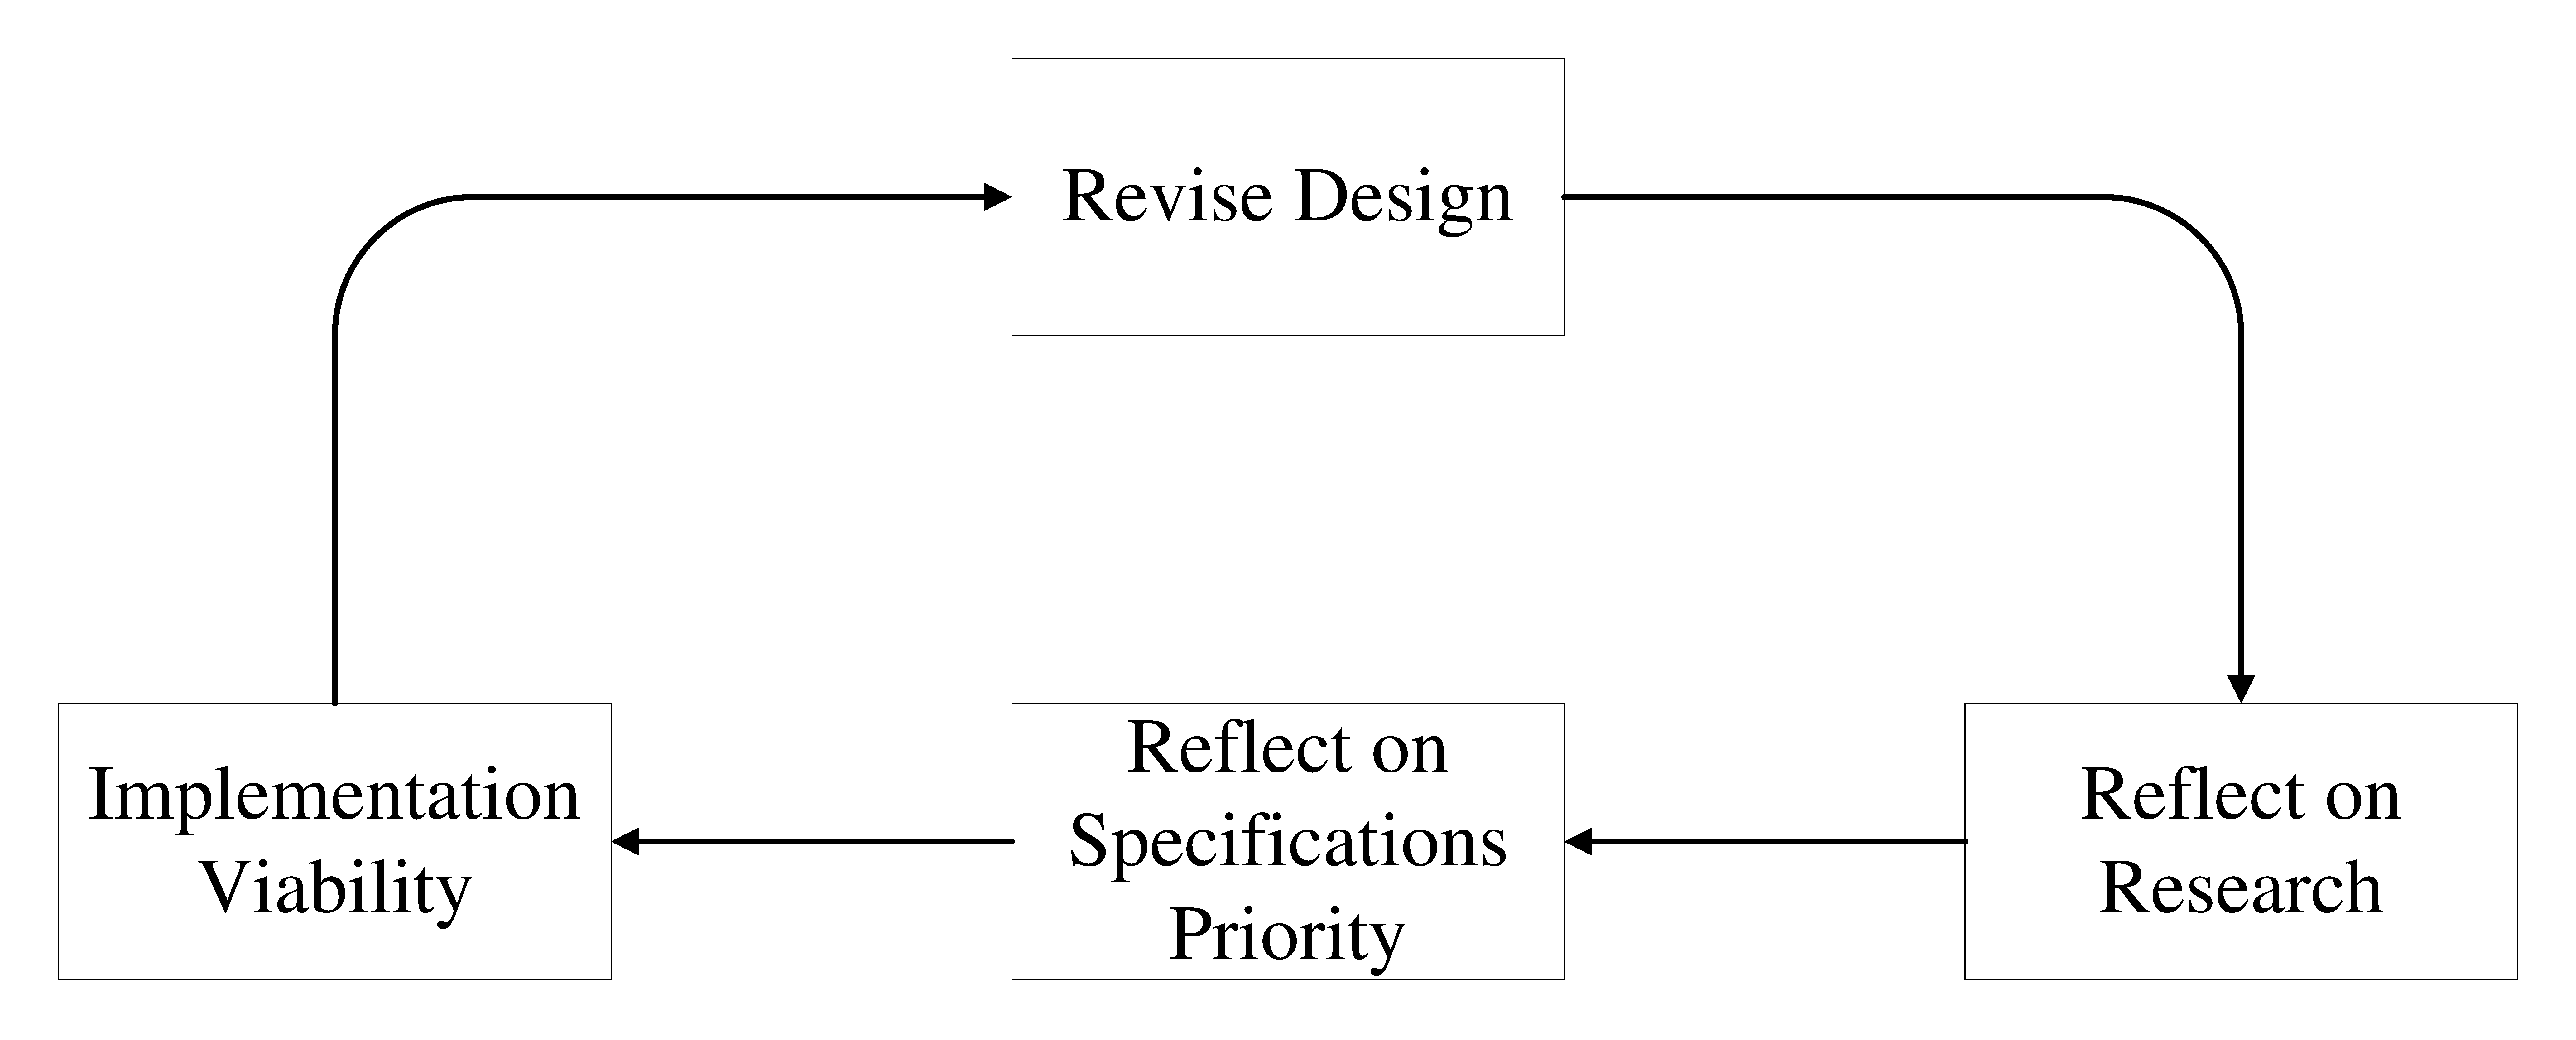
\includegraphics[width=1.0\textwidth]{images/design.pdf}
    \captionsetup{justification=centering}
    \caption[Iterative Design Process]{Iterative Design Process}
    \label{fig:iterative-design}
\end{figure}

\newpage

The focus of this project's design will be on two main components, these components
will have equal importance when it comes to the implementation process.
The first component of the project it is the \acrfull{cc} Server application and the second component
of the project it is the Agent (Client-Side) application.

The Server-Side or the Command and Control (C\&C) component of the project
will allow the establishment of connections for possible clients or agents to its address and to
a specific listening port that will be set by the user. Once a number of agents or clients have been
connected to the Command and Control (C\&C) Server, the remote execution of commands for a potential
client or machine that may require maintenance will be possible.

\section{Command and Control (C\&C)}

The first component of two primary projects components it is the \acrfull{cc} Server which will
support and partially represent the title of the project as this is not the only component required
in order to achieve forecasting of computer systems failure.
The Command and Control (C\&C) Server application will allow the establishment of connections
for possible clients or agents to its address and to specific listening ports that will be set by the user.
Once an agent or client will connect to the Command and Control (C\&C) Server, the Hard-Disk Drive \acrfull{smart}
data will be retrieved and sent back to the \acrfull{cc} for collection. \par
The term \acrfull{cc} refers to a computer which will send directives to digital
devices which were able to establish a connection successfully with the \acrfull{cc}.
In this specific case the digital devices are computer systems which will establish the
connection with the \acrfull{cc} independently on program execution, as the \acrfull{cc}
will allow the creation of agents or clients dynamically with the help of the
cross-platform behaviour of the Java Programming Language by creating Java Archives (.jar)
which will later be deployed on the computers in question which will receive directives. \par
According to Tech Target (2017) a \acrfull{cc} Server type of software it is a software
used to send directives to digital devices which have been infected with malware and the \acrfull{cc}
servers can be used to create networks of devices capable of carrying out cyber attacks such as
Distributed Denial-of-Service (DDoS) or other malicious activities such as stealing of data,
encryption of data and deletion of data in order to perform a specific extortion scheme.
In this specific project, the \acrfull{cc} will not under any circumstances present any of the
security features mentioned previously as the project has the ultimate goal to create a
legitimate and commercial computer systems maintenance tool with a predictive behaviour, yet
it must be considered that the term \acrfull{cc} Server it is most of the time associated with
a malicious type of software and a not a legitimate one, despite the presence of legitimate
and commercial reactive remote desktop maintenance solutions on the market such as AnyDesk and TeamViewer.
The architecture of the \acrfull{cc} will consist of five main elements, these elements are the authentication
system of the application, the interface of the application, the network side of the application, the local
database of the application and last but not the least the collection of \acrfull{smart} data with the ultimate
goal to analyze the data using the machine learning algorithm called \acrfull{svm}.

\subsection{Command and Control (C\&C) Architecture}

\begin{figure}[h]
    \centering
    \includegraphics[width=1.0\textwidth]{images/command-and-control-architecture.pdf}
    \captionsetup{justification=centering}
    \caption[Command and Control (C\&C) Architecture]{Command and Control (C\&C) Architecture}
    \label{fig:command-control-architecture}
\end{figure}

\newpage

\subsection{Unified Modeling Language}

\noindent
\textbf{Use Case Diagram}

\begin{figure}[h]
    \centering
    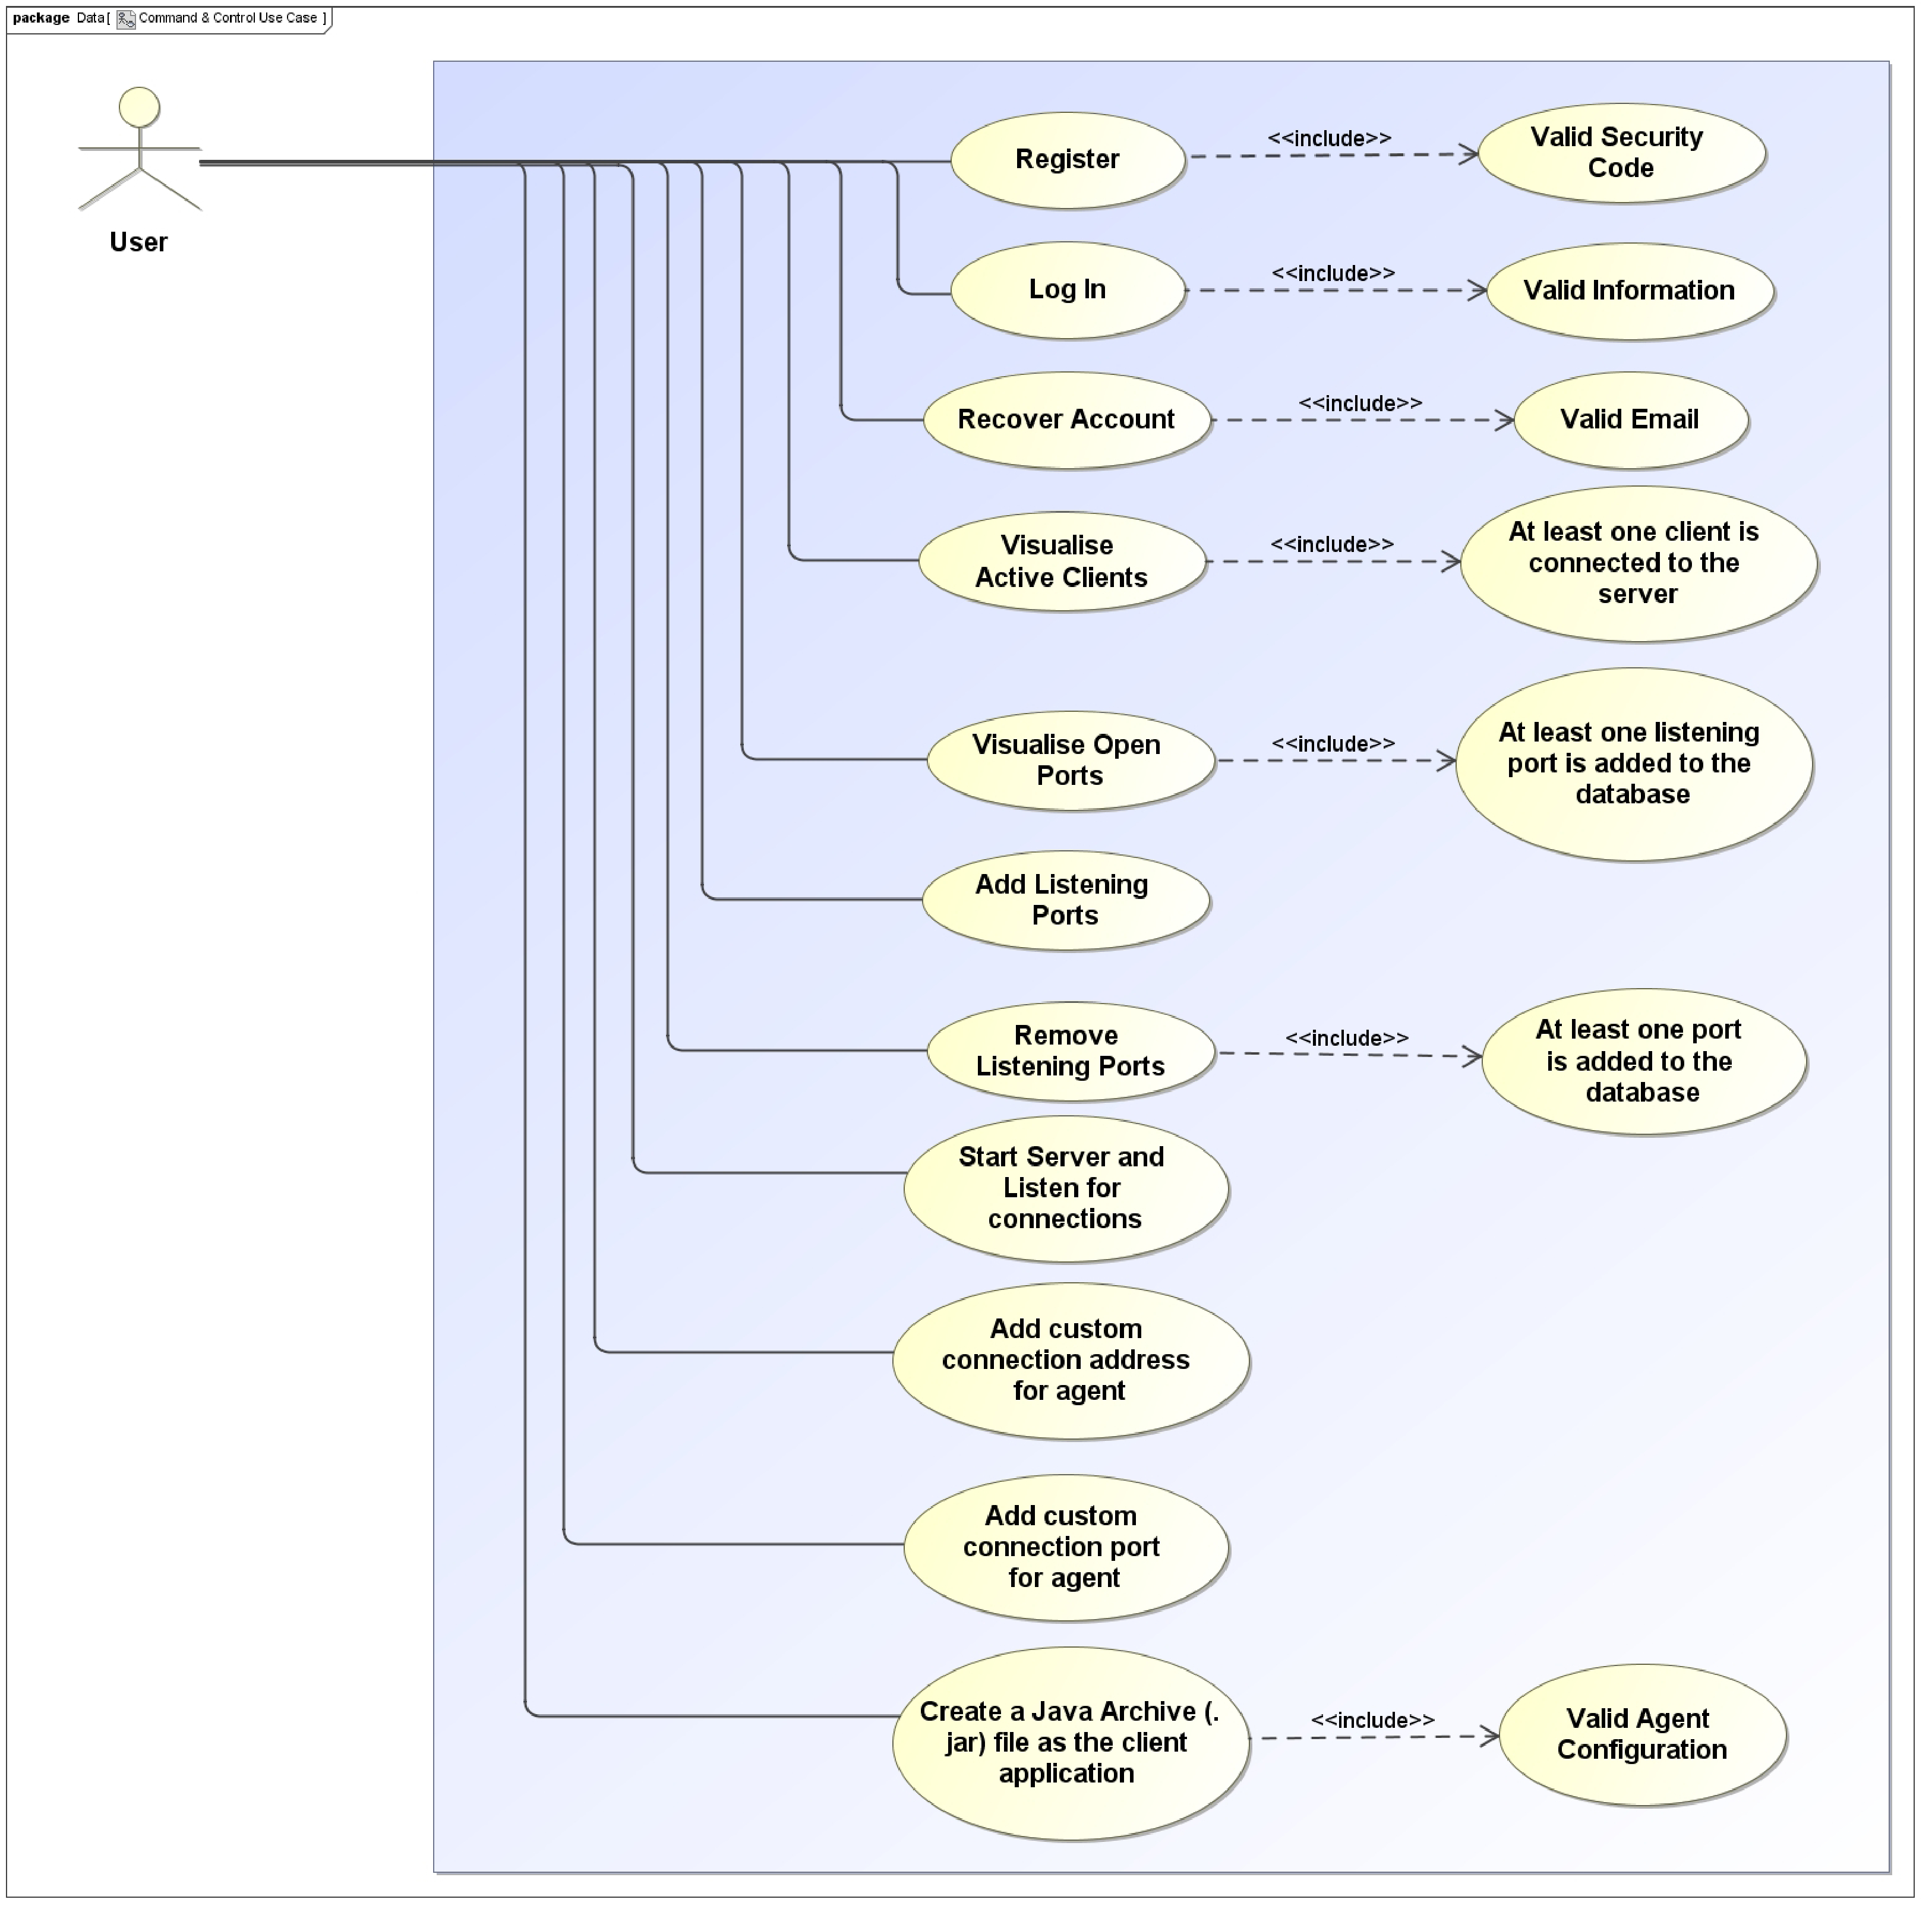
\includegraphics[width=1.0\textwidth, height=0.74\textheight]{images/command-control-use-case.pdf}
    \captionsetup{justification=centering}
    \caption[Command \& Control Application Use Case]{Command \& Control (C\&C) Application Use Case}
    \label{fig:command-use-case}
\end{figure}

The available actions of the \acrfull{cc} Server presented in the figure above represent only
a few of the possible interactions that a user of the desktop application would be able to perform, the most
noticeable and the most vital features of the desktop application presented in the figure above
are the addition of IP addresses, ports to a list of connections and the creation the Java Archive
(.jar) agent.

\newpage

\noindent
\textbf{Activity Diagram}

\begin{figure}[h]
    \centering
    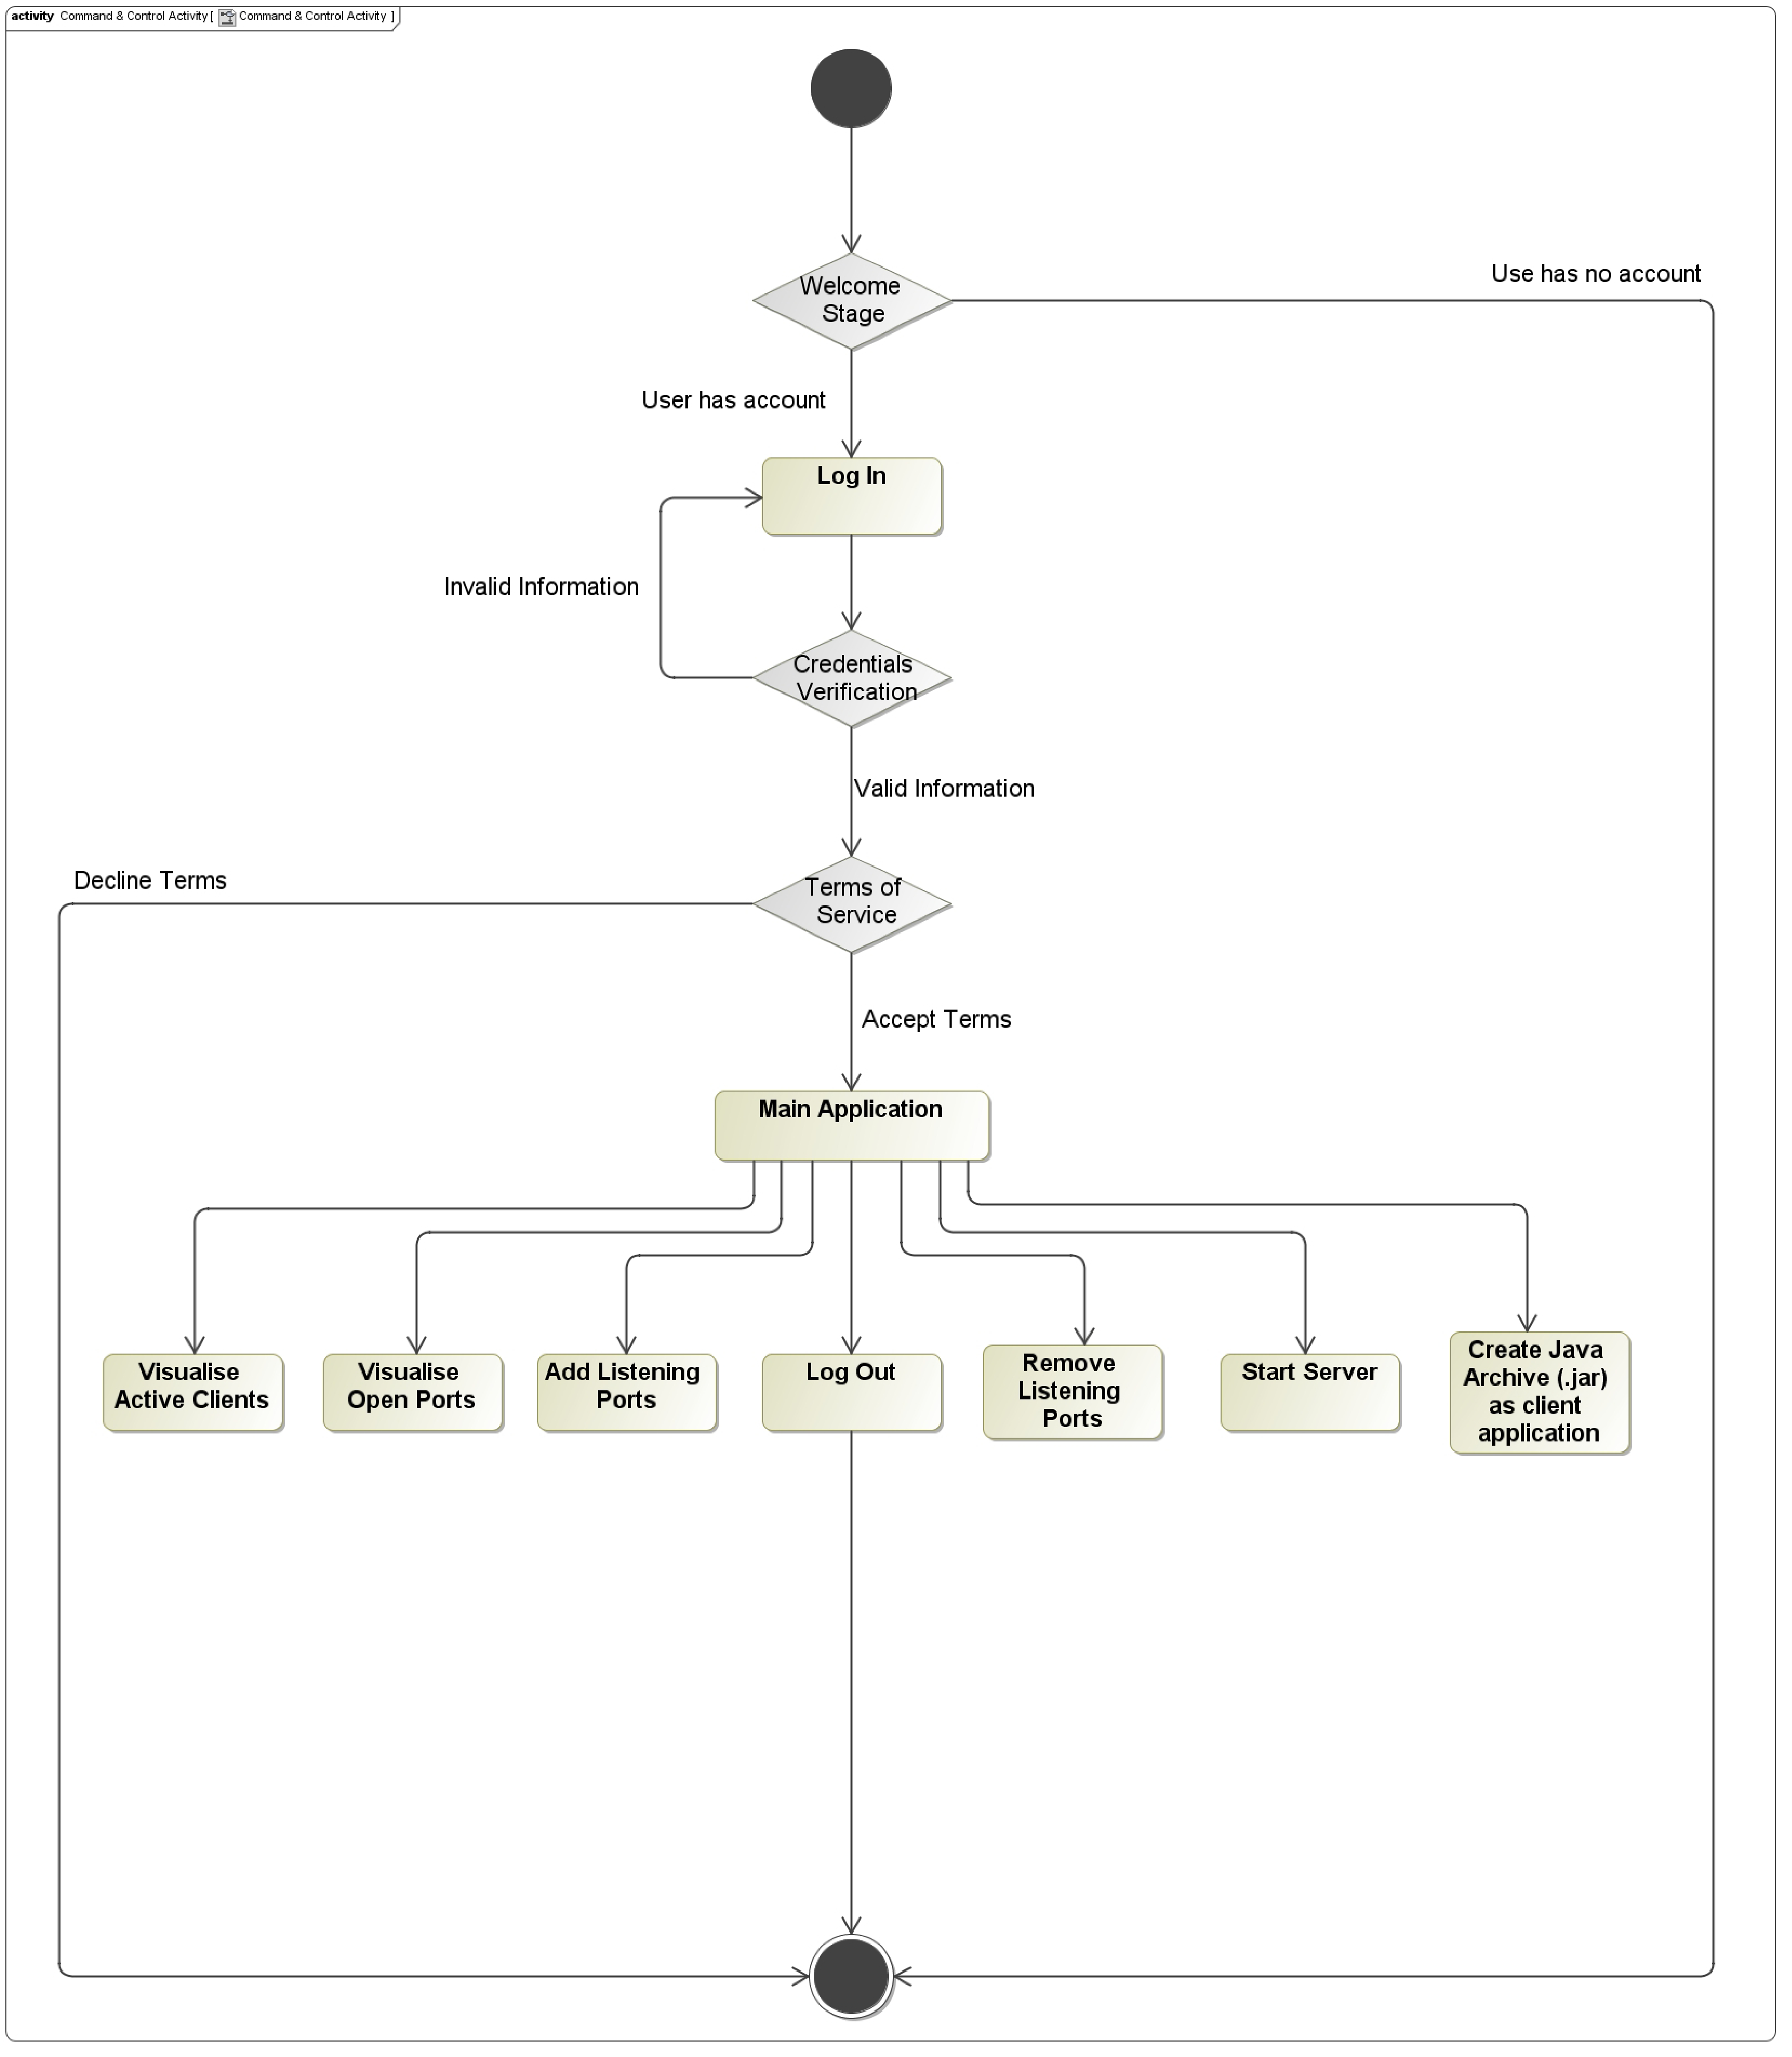
\includegraphics[width=1.0\textwidth, height=0.74\textheight]{images/command-control-activity.pdf}
    \captionsetup{justification=centering}
    \caption[Command \& Control Activity]{Command \& Control (C\&C) Application Activity}
    \label{fig:command-activity}
\end{figure}

The activity flow presented in the figure above represents only a few of the possible interactions
that the user will be presented with, yet comparing to the use case diagram, in this activity flow
the user must perform specific operations in order to reach the main features of the \acrfull{cc}
Server application, these operations are the provision of valid authentication information followed by the
acceptance of the application's terms of service.

\newpage

\noindent
\textbf{Class Diagram}

\begin{figure}[h]
    \centering
    \includegraphics[width=1.0\textwidth]{images/command-control-class-diagram.pdf}
    \captionsetup{justification=centering}
    \caption[Command \& Control Class]{Command \& Control (C\&C) Application Class}
    \label{fig:command-class}
\end{figure}

The \acrfull{cc} Server Application it is a Desktop Application with a decent level of
complexity containing multiple Java Classes, in the figure presented above only a few of
those classes are shown, the Java Classes shown in the class diagram from above are classes
considered to be at the core of the \acrfull{cc} Server Desktop Application. The Graphical User
Interface of the \acrfull{cc} will be built using the JavaFX Interface Framework in association
with the MigLayout container which it is a grid based type of container with the potential to
achieve even the most complex types of layout without the need of using other nested types of
JavaFX build-in layouts such as BorderPane, HorizontalBox and VerticalBox. In the
figure \ref{fig:command-class} it can be seen that all Panels inherit the features
of the MigLayout Container in order to organize the structure of the \acrfull{cc} Server
application. The predominant connector presented in the Figure \ref{fig:command-class}
it is the Composition connector which will imply the mandatory existence of the associated
Classes. The only non-graphical Class presented in the Figure \ref{fig:command-class} it is
the TCPServer Class which has the role to create an independent listening server object
running on a separate Thread of the Main JavafX Thread in order to allow for a smooth
execution of operations without any interruptions, this Class will allow the establishment
of connections from Agents or Clients on a specific IP Address and a specific Port set by
the user using the Graphical User Interface. In addition to the listening operation of
the Server Socket, the TCPServer Class will also allow the reset of all current connections
using the "running" boolean attribute which can be set to true in order to start the
Server or false to stop the server, this will be done with the help of the Class Getters
and Setters, which will be used in the Network Panel to control this type of events.

\newpage

\noindent
\textbf{Sequence Diagram}

\begin{figure}[h]
    \centering
    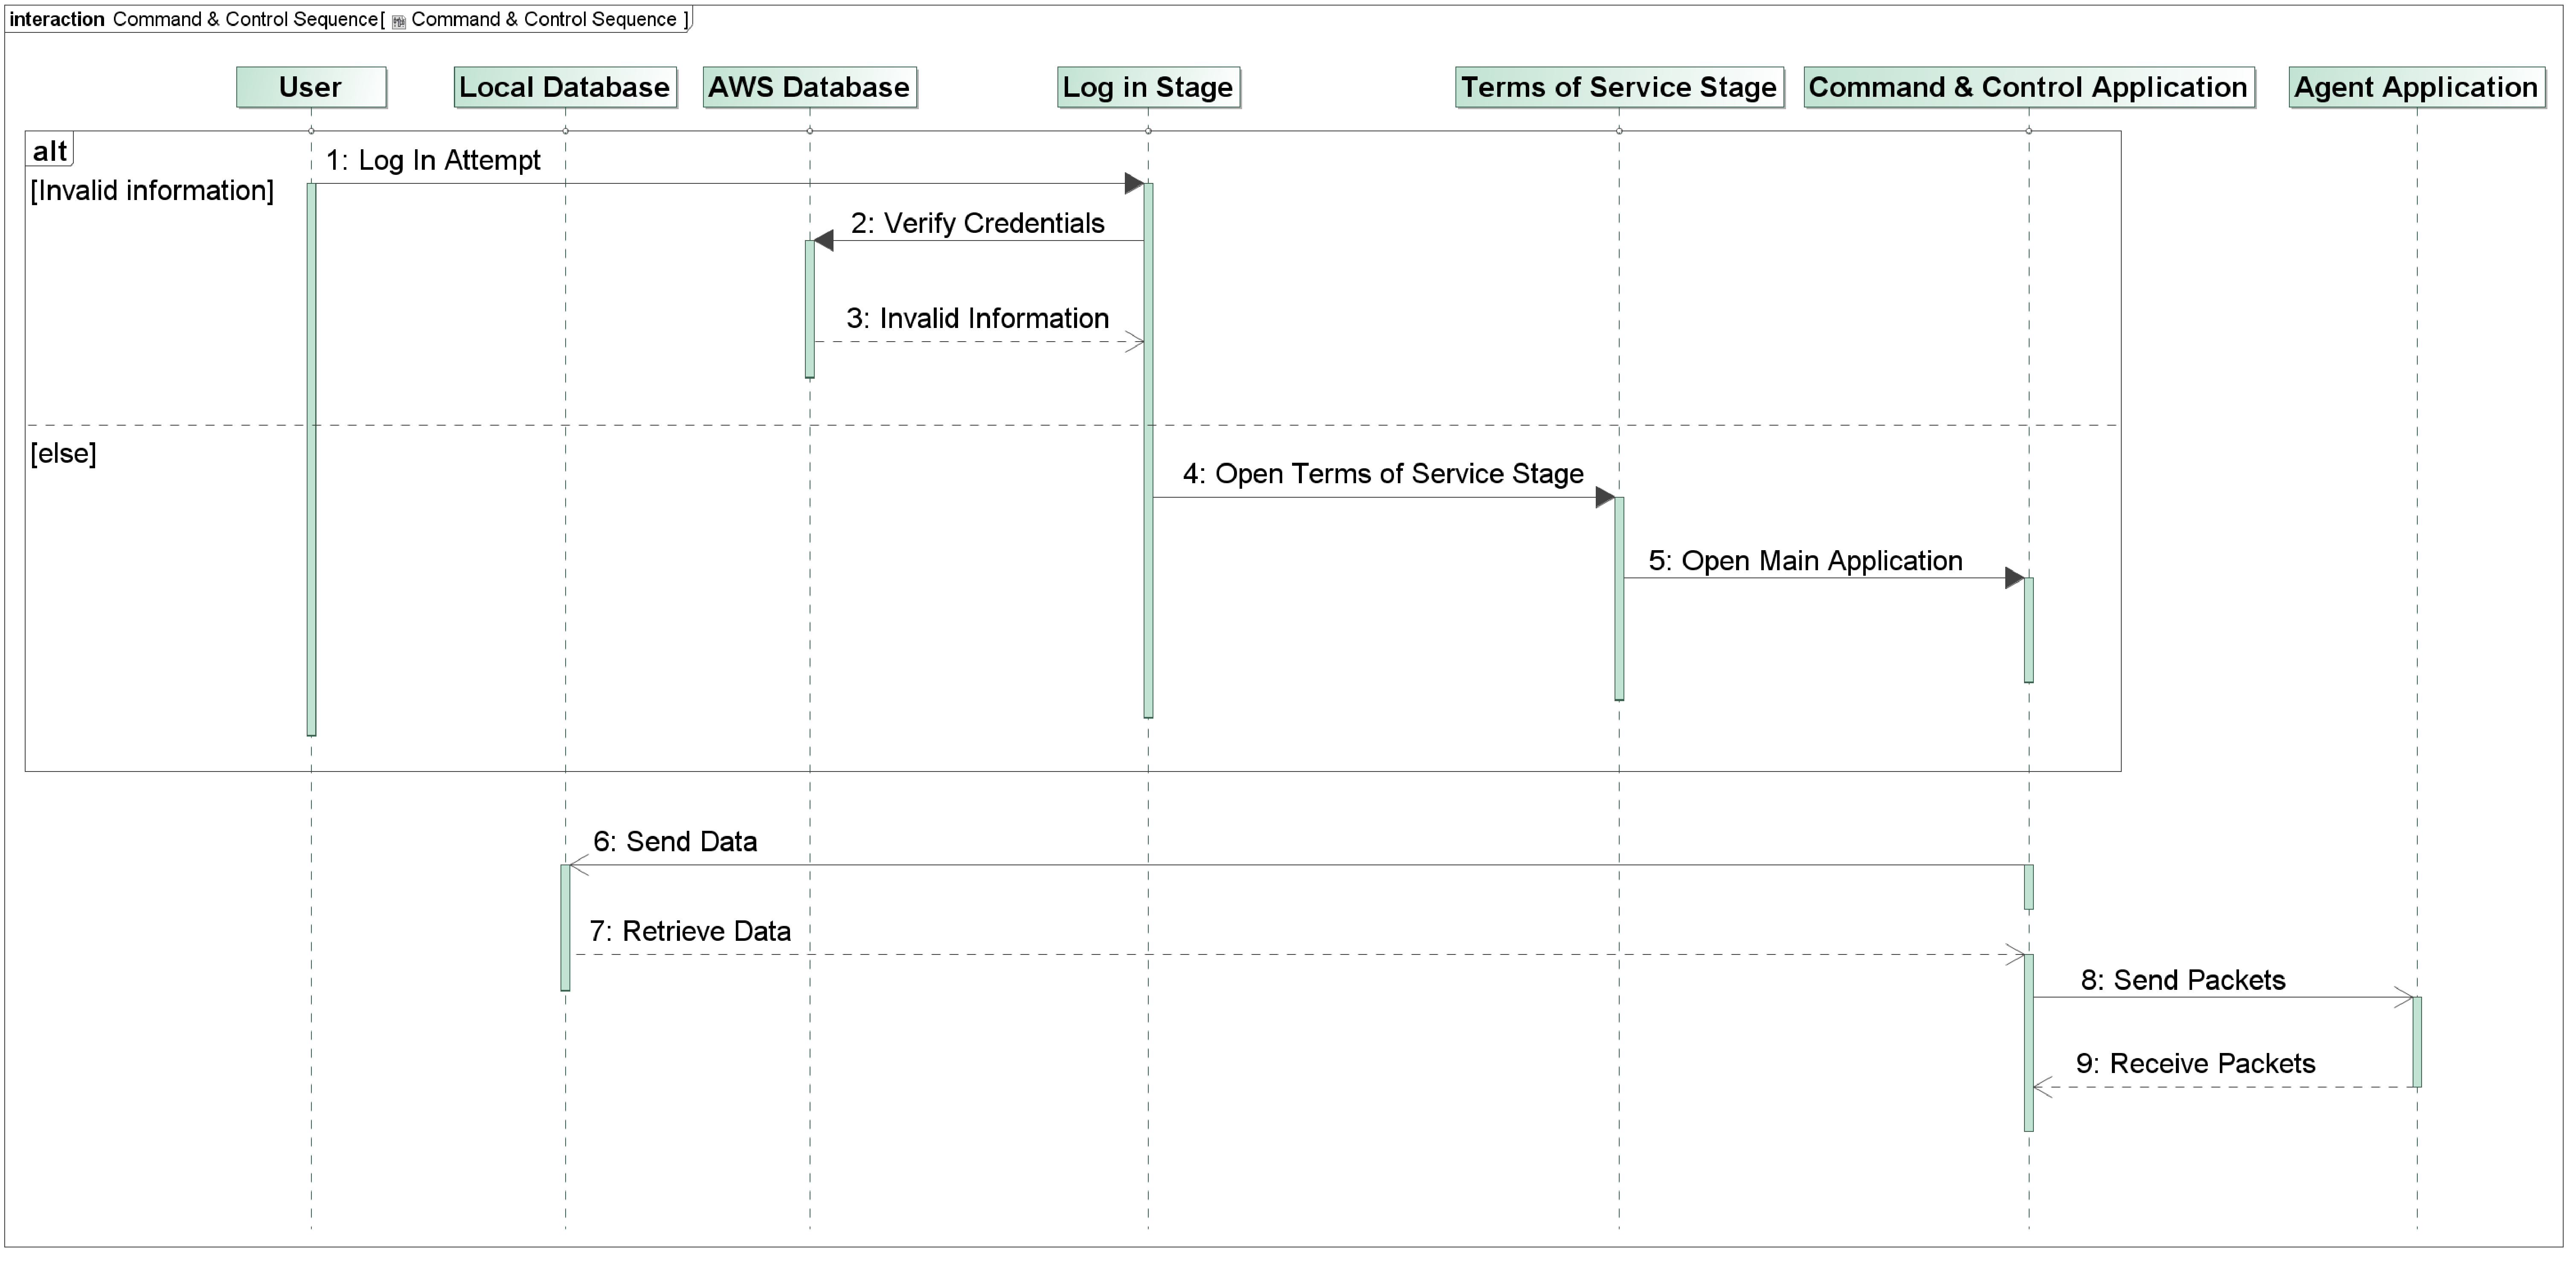
\includegraphics[width=1.0\textwidth]{images/command-control-sequence.pdf}
    \captionsetup{justification=centering}
    \caption[Command \& Control Sequence]{Command \& Control (C\&C) Application Sequence}
    \label{fig:command-sequence}
\end{figure}

The figure \ref{fig:command-sequence} represents the sequence of events between the main
entities of the project. The entities presented in this diagram are the User entitiy,
the local SQLite database entity, the Cloud Amazon Cognito database entity, the JavaFX Log in Stage,
entity, the JavaFX Terms of Service Stage entity, the \acrfull{cc} Server Application Stage
entity and last but not the least the Agent (Client-Side) Application entity which will
interact with the \acrfull{cc} Server Application if a series of events would happen.
The two most important entities in this diagram are the \acrfull{cc} Application and the
Agent Application. In order to have a sequence of events between the two most important
mentioned entities, a series of events must happen in a specific order. The first event
would be the user attempt to log in using the JavaFX Log in Stage, the second event would be the verification
of user credentials against the Cloud Amazon Cognito database, if the credentials are invalid,
then the user would not be able to access the JavaFX Terms of Service Stage, this being the
third event and the response from the Cloud Amazon Cognito database. However, if the
user would enter valid credentials, the JavaFX Terms of Service would be prompted, this being
the fourth event in the sequence. Once the JavaFX Terms of Service would be shown, the user
would be able to accept the terms shown to move to the main \acrfull{cc} Server Application,
where specific could ports associated with a password will be added to the local SQLite
database and the communication with the Agent (Client-Side) would be possible in the form
of sending packets and receiving packets between the two main applications (\acrfull{cc}
Server Application and Agent (Client-Side) Application).

\newpage

\subsection{Controller of Application}

\begin{figure}[h]
    \centering
    \includegraphics[width=1.0\textwidth]{images/command-and-control-controller.pdf}
    \captionsetup{justification=centering}
    \caption[Command \& Control Controller Components]{Command \& Control (C\&C) Application Controller Components}
    \label{fig:command-controller}
\end{figure}

In the figure \ref{fig:command-controller} it can be seen the architecture of the \acrfull{cc}
Server Application with close look at the controller part of the Application, the two
elements presented beside the \acrfull{cc} Server Controller are the View of the Application
or the JavaFX Interface and the Models used though the whole application as a shared
faeture between the JavaFX Interface and the Controller.
The main elements within the controller of the \acrfull{cc} Server Application are the Amazon Cognito Database,
the Network Sockets and Streams, the local SQLite database and the agent builder which
is composed from multiple components which are not shown in the \ref{fig:command-controller}.
However, the agent builder is composed of two main components which will be discussed largely
in the implementation chapter, the first component would be the configuration aspect of the agent
which concerns the IP or DNS (Domain Name System) address and the port to which the agent
should connect to and the second component would be the creation of the agent into a
Java Archive (.jar) with the associated configuration. The configuration of the agent
would be created dynamically using the ASM Java Bytecode Manipulation library from
France Telecom which will allow the modification of a Java class by changing the values
of simple class constants to values used in specific class methods and even more as the
library offers extended functionality for the manipulation of Java Classes.

\newpage

\subsection{Interface of Application}

\begin{figure}[h]
    \centering
    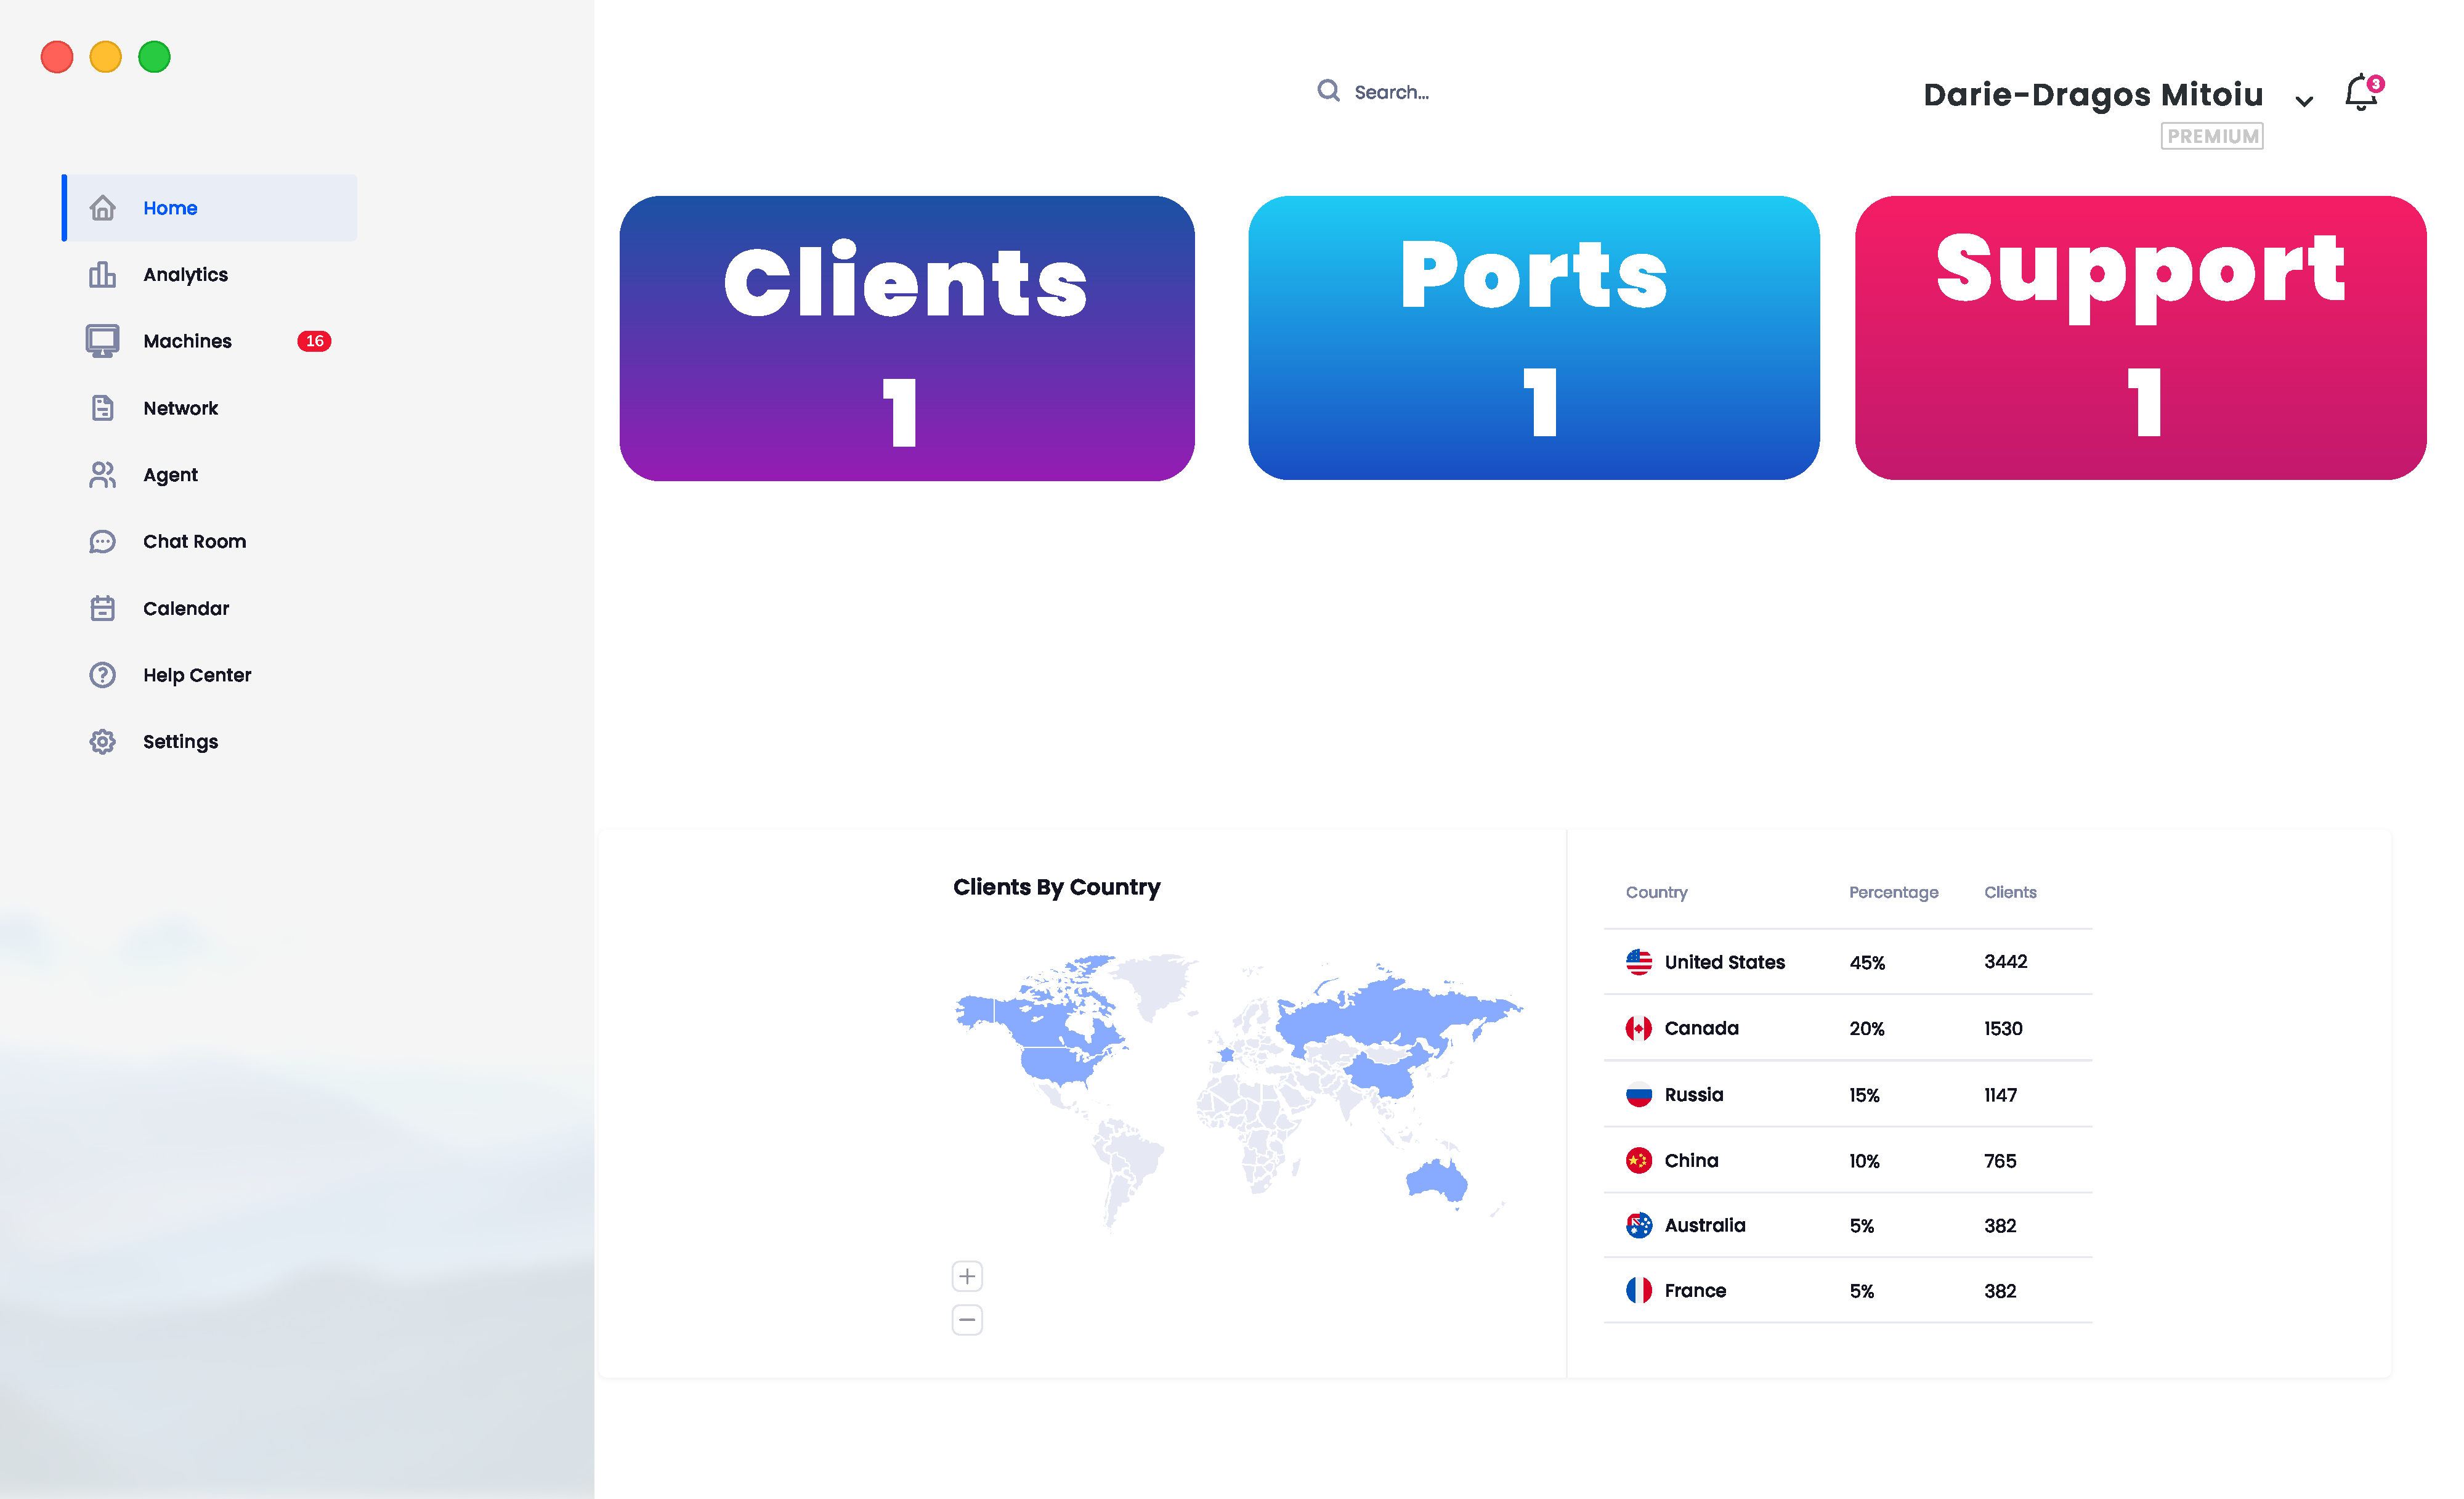
\includegraphics[width=1.0\textwidth]{images/command-control-dashboard.pdf}
    \captionsetup{justification=centering}
    \caption[Command \& Control Dashboard Design]{Command \& Control (C\&C) Application Dashboard Design}
    \label{fig:command-dashboard}
\end{figure}

The partial interface of the \acrfull{cc} Server application presented in the \ref{fig:command-dashboard}
was produced through numerous design iterations which have allowed a series of features
to be presented in the final design result. The \ref{fig:command-dashboard} represents
the dashboard panel of the \acrfull{cc} Server Application which has been mentioned in the
specifications chapter. The overall interface it is presented into a JavFX Stage with
a vertical side menu presented on the left side of the window and the content of the
dashboard panel on the right side of the window. The design presented in the \ref{fig:command-dashboard}
follows the two-column design approach, where the first grid column it is represented by the
vertical side-menu and the second grid column it is represented by the selection made
on the vertical side-menu as each options will replace the content on the right side
of the window on button press. In addition to the general presentation, the JavFX Stage
also contains a minimize, expand and close window buttons situated on the left side of
the window bar, these buttons can be placed either on the left side of the window bar
or on the right side of the window bar due to the extensive capabilities of the JavaFX
interface framework. When it comes to the content of the window, the side-menu contains
eight menu elements, the first one being the Home element or the dashboard element which
will show the number of clients or agents connected to the \acrfull{cc} Server Application,
the number of ports opened by the \acrfull{cc} Server Application, the number of clients
or agents that may require support based on the Hard-Disk Drive \acrfull{smart}
indicators and last but not the least a world map situated below the session data
containing the number of agents connected to the \acrfull{cc} Server Application based
on their geographical location.

\newpage

\section{Agent (Client-Side)}

The component of the project will be the Agent component or the Client-Side application of which
will be created in a dynamic way by the Server-Side or Command and Control (C\&C) Desktop Application
using an IP address and a port specified by the user at the moment of agent creation.
The Agent or the Client created will ultimately be responsible for sending relevant information to
the Command and Control (C\&C) Server, which in this specific case, the data in question it is the
Hard-Disk Drive \acrfull{smart} attributes and potentially executing specific instructions on the client
machine which will be sent or instructed by the Command and Control (C\&C) Server Application.
The architecture of the Agent or Client application will consist of four main elements, these elements are the command
line interface of the application, the network side of the application, the Java Bytecode
configuration of the application and last but not the least the smartmontools third-party application
which will allow the Hard-Disk Drive \acrfull{smart} data to be retrieved and sent to the
\acrfull{cc} Server application.

\subsection{Agent (Client-Side) Architecture}

\begin{figure}[h]
    \centering
    \includegraphics[width=1.0\textwidth]{images/agent-architecture.pdf}
    \captionsetup{justification=centering}
    \caption[Agent (Client-Side) Architecture]{Agent (Client-Side) Architecture}
    \label{fig:agent-architecture}
\end{figure}

\newpage

\subsection{Controller of Application}

\begin{figure}[h]
    \centering
    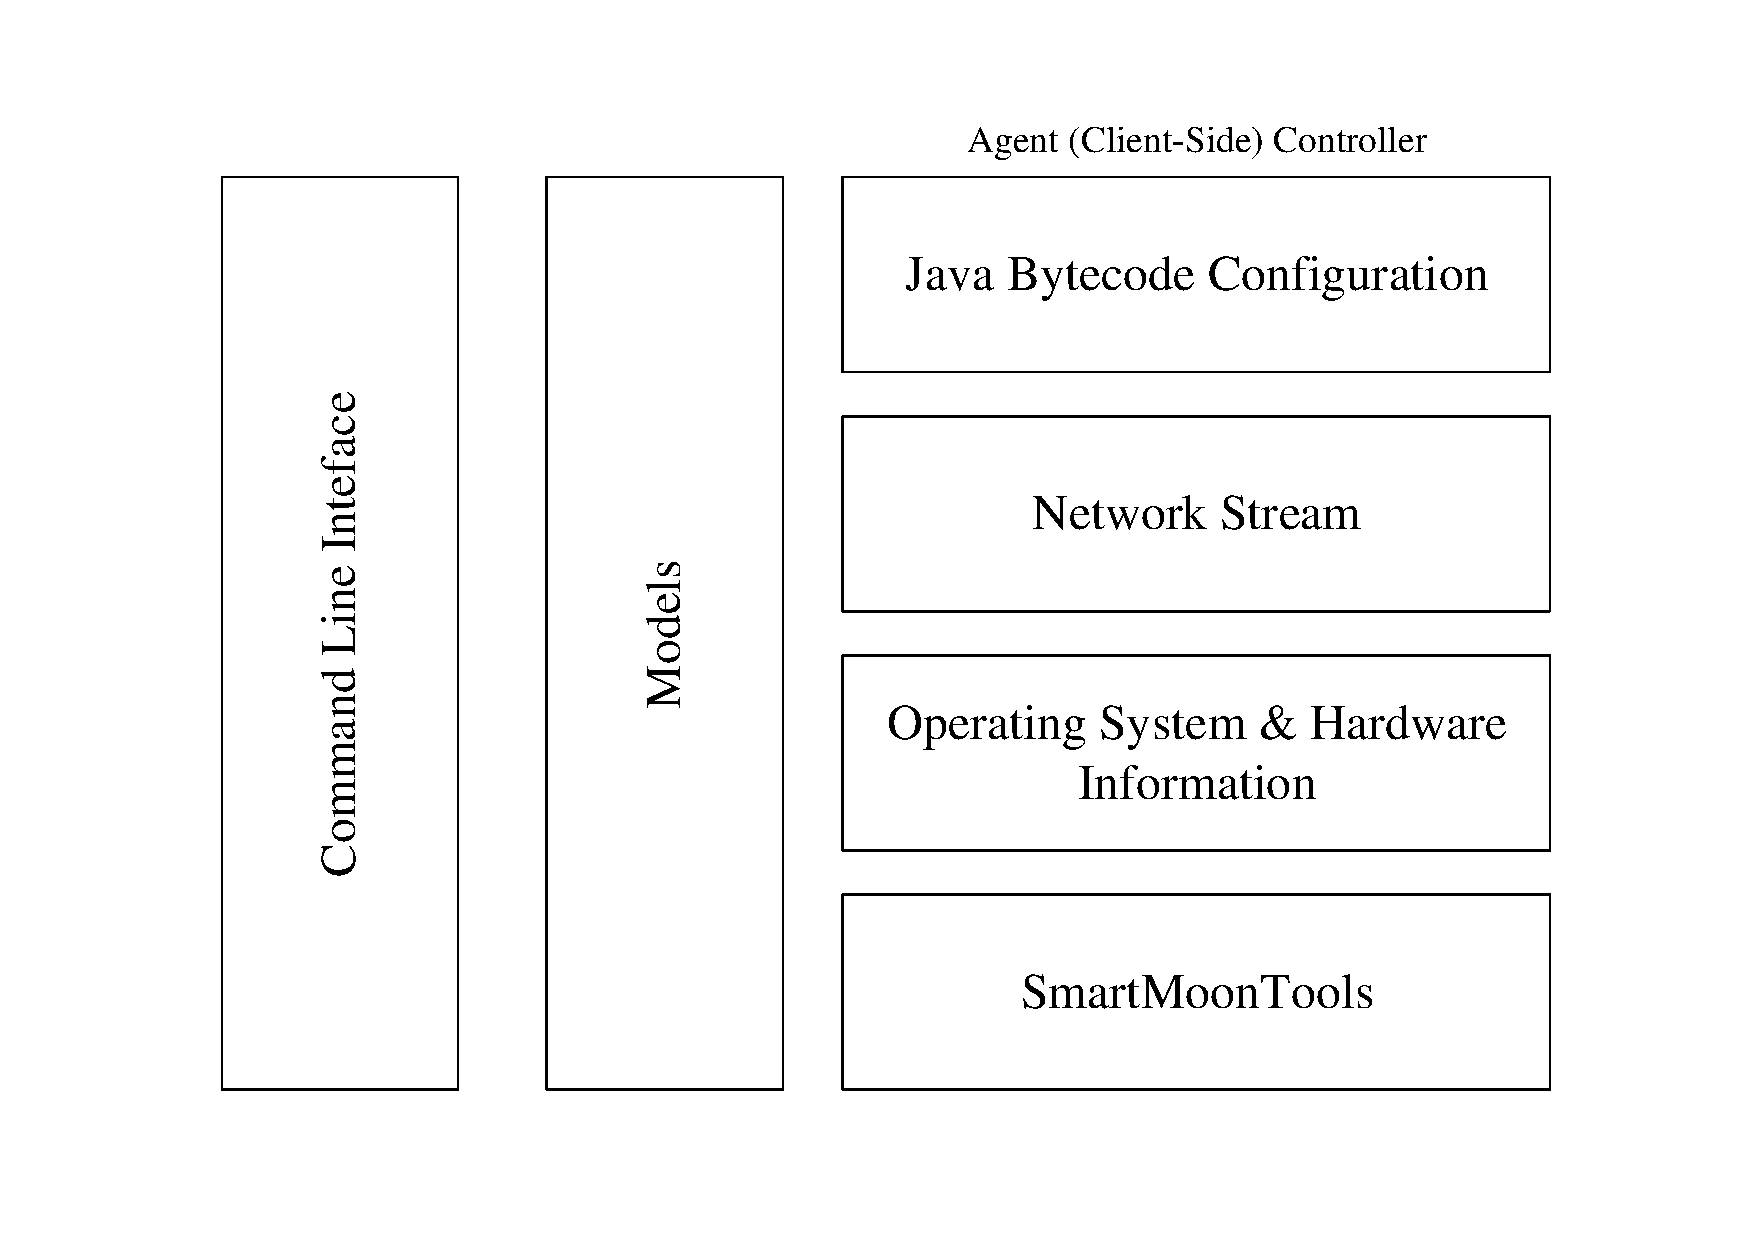
\includegraphics[width=1.0\textwidth]{images/agent-controller.pdf}
    \captionsetup{justification=centering}
    \caption[Agent (Client-Side) Controller]{Agent (Client-Side) Controller}
    \label{fig:agent-controller}
\end{figure}

In the figure \ref{fig:agent-controller} it can be seen the architecture of the Agent (Client-Side)
application with a focus on the controller of the application. The first two elements
presented in the figure \ref{fig:agent-controller} are the command line interface of the
Agent (Client-Side) and the models used through the whole Agent (Client-Side) sub-project.
The main elements presented in the Agent (Client-Side) Controller are the Java Bytecode
Configuration, the Network Socket and input, output Streams, the ability to retrieve
Operating Systems and Hardware information and the utilisation of the third-party
application called Smartmontools. The Java Bytecode Configuration element refers to
a dynamically created Java Class containing the IP or DNS (Domain Name System) address
and the port specified at the creation of the agent using the \acrfull{cc} Server
Application. The Network Stream element refers to the Object Input Stream and the Object
Output Stream used to send and receive data to and from the \acrfull{cc} Server
Application. The Operating System \& Hardware Information element refers to the ability
to retrieve Operating System \& Hardware Information either with the default behaviour
of the Java Programming Language or with the help of the third-party libraries mentioned
in the specifcations chapter. The Smartmontools element refers to the involvement of the
third-party application called Smartmontools which must be installed on the machine
which will execute the Agent (Client-Side) Application in order to retrieve and send
the Hard-Disk Drive \acrfull{smart} data to the \acrfull{cc} Server Application.


    \chapter{Implementation}
    In this chapter of the document, the architectural decisions presented in the previous chapter will taken
forward into building the mentioned artifacts in association with the experiments necessary in order to
prove the forecasting aspect of computer systems failure by making use of machine learning techniques
such as the \acrfull{svm} algorithm. In addition, this chapter will cover specific implementation
decisions in order to solve the problem of forecasting computer systems with the help of machine
learning techniques. The implementation chapter will contain three main sections which will aim
at the most important aspects of the project, these three main sections are the \acrfull{cc} Server
Application part of the project, the Agent (Client-Side) part of the project and the Machine Learning
aspect of the project. The \acrfull{cc} Server Application section of the chapter will contain a series
of sub-sections, these sub-sections will discuss the Interface of the application, the Controller of the
application, the Amazon Cognito Authentication Database, the local SQLite Database, the networking programming
aspect of the application, the collection of Hard-Disk Drive \acrfull{smart} data aspect of the application and the
specific interactions with the Agent (Client-Side) application, the security aspect of the application
and last but not the least the testing approach for the features of the application. The Interface sub-section
of the \acrfull{cc} Server Application will also contain a series of sub-sub-sections which will aim at
discussing the benefits of using the JavaFX Interface Framework in association with the Model-View-Controller
architectural structure over the older Interface framework called Swing. The Agent (Client-Side) section will
contain a series of sub-sections, these sub-sections are the controller of the application, the networking
programming aspect of the application, the security apspect of the application and last but not the least
the testing approach taken for the features of the application. The third main section of the implementation
chapter it is the Machine Learning section which will focus on a static analysis of a BackBlaze Hard-Disk
Drive \acrfull{smart} data from a single vendor of Hard-Disk components in order to have accurate predictions.
The Machine Learning section will contain a series of sub-sections which are data exploration, data pre-processing
and classification.

\section{Command and Control (C\&C)}

The \acrfull{cc} Server Application it is structured into three main architectural components based
on the Model-View-Controller architecture. The View or the Interface of the application it is a
JavaFX based Interface while the Models and the Controller of the application do not present any
special mentions in their composition. The Controller of the application handles the networking aspect
of the application, the Amazon Cognito Authentication Database and the local SQLite Database, while
the Models part of the application it is a shared component between the View and the Controller of the
application.

\subsection{Model-View-Controller}

The Model-View-Controller (MVC) it is an architectural pattern which will allow
the separation of the application logic into three main components, these components are
called Model, View and Controller, usually these names will be used for package names in
a Java project. The three components mentioned are designed to handle specific development
aspects of the application. This architectural pattern will allow the creation of extensible
and scalable applications. The pattern it is used most of the time for web development
project, but is not limited to this usage, as many desktop applications and mobile applications
projects can be structured to use the same architectural pattern with success. \newline

\noindent
\textbf{Model}
\newline

The Model element in a Model-View-Controller Architecture pattern represents a Java
Object carrying data, this object can also have a logical controller with the role to
modify necessary data. The Model component represents all data related logic that the
developer will use for the development of the application. This aspect can represent
any application logic related data or just data which is passed between the view and
controller. \newline

\noindent
\textbf{View}
\newline

The View element represents the visualisation method of the data that the
model contains. The View element can be interpreted as the Interface code container
of the application. The view component it is used for the graphical user interface
aspect of the application, e.g: labels, text fields, dropdown menus etc. \newline

\noindent
\textbf{Controller}
\newline

The Controller element will act as both model and view as it controls the data flow into
the model object and eventually it will update the view whenever the data will change, this
aspect separates the view and model elements. The controller component will behave as an
intermediary between the model and the view components in order to process all application
logic and incoming requests to manipulate necessary data using the required model and then
interact with the view or graphical user interface component to show some visual content.

\newpage

\subsection{Graphical User Interface}

In the background chapter it was seen that the machine learning algorithm called
\acrfull{hmm} it is a statistical machine algorithm used for anomaly detection
which in the case of the research papers investigated was implemented using the
Java Programming Language. In the specifications chapter, the initiative of using
the Java Programming Language was followed, but in the functional requirements
mentioned in the specifications chapter have been created with the utilisation
of the machine learning algorithm called \acrfull{svm} in association with the
Hard-Disk Drive \acrfull{smart} indicators. This being said, the involvement of
the Java Programming Language offers a rich set of libraries or frameworks
to create Graphical User Interfaces in a platform independent way, there are
two libraries that stand out in terms of functionality and can be considered as
main options when it comes to the design and implementation of the \acrfull{cc}
Server Application, these two options are the Swing Interface Framework and the
JavaFX Interface Framework. The Swing Interface Framework can be integrated with
the JavaFX Interface Framework and vice-versa in order to create rich, custom
and interchangeable interfaces due to the interoperability offered by both
Interface Frameworks. An example of such interoperability would be to use
these two Interface Frameworks together to have a Swing Frame and multiple
JavaFX Widgets in that frame if the JFXPanel container is used and added
to the Swing Frame. The Swing Interface Framework or API it is a set of
extensible Interface components designed to ease the process of creating
rich and custom Java based Graphical User Interfaces, the Swing Framework
or \acrfull{api} it is build on top of an older Interface Framework called
\acrfull{awt} and since the \acrfull{awt} it is an even older Java Interface
Framework, the Swing Framework acts as replacement of the \acrfull{awt}
Framework or \acrfull{api} as it has most of the \acrfull{awt} graphical
widgets or components. The Swing Interface Framework also complies with
the Model-View-Controller architecture which will eventually respect
elements such as: An Interface Framework or Graphical \acrfull{api} will
suffice to support multiple platforms aspects and an Interface Framework
or Graphical \acrfull{api} will be model driven so no data should be
involved in the highest level \acrfull{api}. The JavaFX Framework also
follows a similar pattern to the Swing Framework and it is a Framework
which can create applications with a more appealing visual aspect comparing
to the Swing Framework.
The \acrfull{cc} Server Application will be implemented using the JavaFX
Graphical User Interface due to the modern feel and look comparing to the
Swing Framework. However, the interoperability between the two Graphical
User Interface Frameworks will allow the interchangeability of the interface
components really easy. Both Swing and JavaFX Graphical User Interface will
allow the project to be structured into a Model-View-Controller architecture
pattern, nevertheless, the JavaFX Graphical User Interface Framework can be
apprached using the Model-View-Controller in two ways, either by making use
of the FXML feature which will be discussed in the following sections, or
the creation of the view using pure Java code which is more suitable for dynamic
and interactive Graphical User Interfaces.

\newpage

\subsubsection{Swing}

The Java Swing Interface Framework presents a list of features when it comes
to the ability to create rich and custom Graphical User Interfaces, these
features are the following: \newline

\noindent
\textbf{Light Weight}
\newline

The Swing Interface components or widgets do not rely on the Operating System to function as the
components are independent of the Operating Systems's \acrfull{api}, the widgets being
created and rendered using the pure Java Cross-Platform instead of relying on Operating
System calls. \newline

\noindent
\textbf{Rich Controls}
\newline

The Swing Interface components or widgets offer a rich set of controls which can be considered
as advanced or with a high degree of complexity, e.g: JTree, JTabbedPane, JSlider,
JColorChooser and JTable. \newline

\noindent
\textbf{Highly Customizable}
\newline

The Swing Interface components or widgets offer a highly customizable behaviour in a very
easy manner when it comes to the visual appearance due to the independent aspect of
internal representation. \newline

\noindent
\textbf{Pluggable look-and-feel}
\newline

The Swing Interface components or widgets offer the ability to change the visual look and
feel at run-time based on specific values, meaning the widgets can have specific visual
appearance for the Operating Systems the application is running on.

\subsubsection{JavaFX}

The technology called JavaFX it is a framework or library used to create Rich Internet
Applications. The JavaFX applcations will be by default cross-platform applications due to
the involvement of the Java Programming Language. In addition, the applications which are
built using the JavaFX Interface Framework can run on devices such as Desktop Computers,
Mobile Phones, Tablets and TVs. In order to develop rich Graphical User Interfaces using
the Java Programming Language, software developers have relied for many years on Interface
Frameworks such as \acrfull{awt} and Swing. However, with the release of the JavaFX
Interface Framework, the software developers not only they can develop new applications
using the newly created Framework, the older applications wrote in \acrfull{awt} and Swing
can be integrated with the JavaFX Interface Framework due to the interoperability mentioned
in the previous sections.

\newpage

The JavaFX Interface Framework presents a list of features when it comes
to the ability to create rich and custom Graphical User Interfaces, these
features are the following: \newline

\noindent
\textbf{FXML}
\newline

The JavaFX Interface Framework presents a feature known as FXML which is a language
similar to HTML which has the role to define static user interface components. \newline

\noindent
\textbf{Swing Interoperability}
\newline

The JavaFX Interface Framework allows the integration of Swing components or widgets using
the Swing Node Class, this interoperability can also work the other way around where Swing
application can allow the integration of JavaFX components or widgets using the JavaFX
Node Class. \newline

\noindent
\textbf{Build-In User Interface Controls}
\newline

The JavaFX Interface Framework presents a list of Build-In User Interface controls or
components which will allow the creation of rich and full featured applications. \newline

\noindent
\textbf{Cascade Style Sheet}
\newline

The JavaFX Interface Framework allows the utilisation of the CSS (Cascade Style Sheets)
for the style of the application, the use of the CSS (Cascade Style Sheets) allows the
design and styling of the application to be done in an easy manner due to the common
aspect of the CSS (Cascade Style Sheet) this styling method being used extensively in
web development. \newline

\noindent
\textbf{RIch Set of APIs}
\newline

The JavaFX Interface Framework offers the ability to access a series of Java Platform
capabilities such as Java Language annotations, generics multi-threading, lambda
expressions in order to create rich Graphical User Interfaces. \newline

\noindent
\textbf{Integrated Graphics}
\newline

The JavaFX Interface Framework offers the ability to use specific Classes for two-dimensional
and three-dimensional graphics. \newline

\noindent
\textbf{Graphics Pipeline}
\newline

The JavaFX Interface Framework offers the graphics accelerator called Hardware accelerated
graphics pipeline also known as Prism. If the Graphics Processing Unit (GPU)
supports this feature, the graphical experience will be a smooth one.

\newpage

\begin{figure}[h]
    \centering
    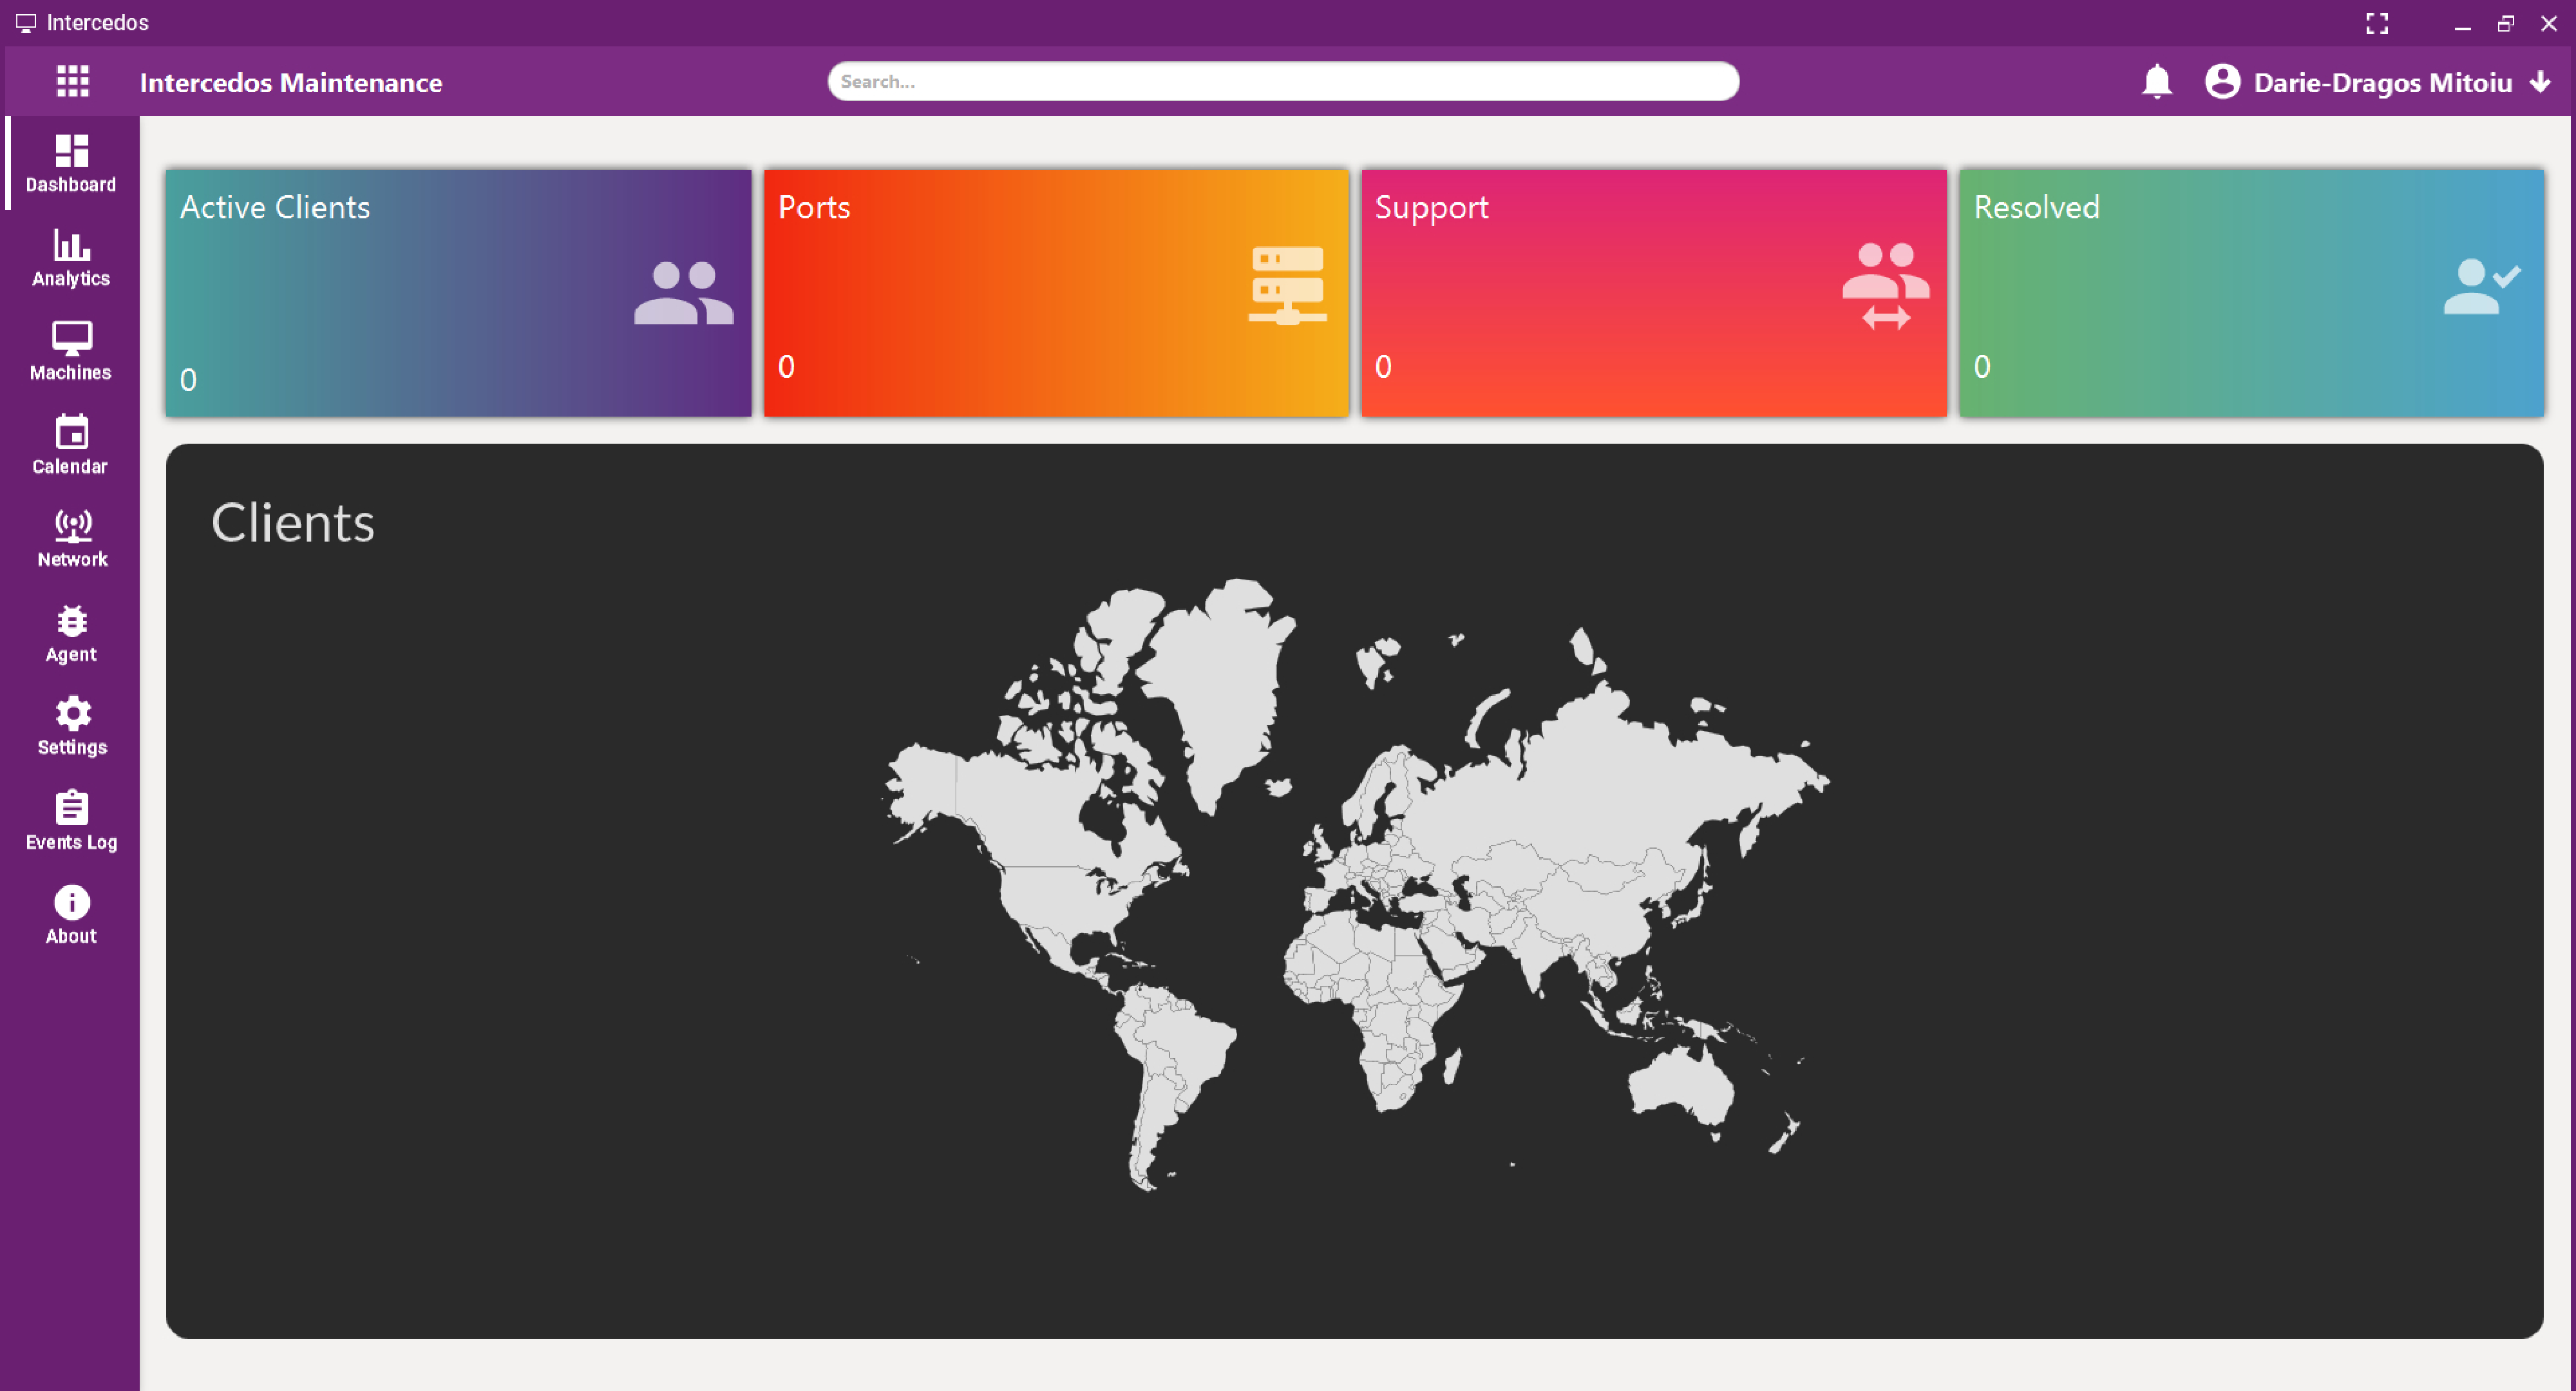
\includegraphics[width=1.0\textwidth]{images/dashboard-light-theme.pdf}
    \captionsetup{justification=centering}
    \caption[Command and Control (C\&C) Light Theme]{Command and Control (C\&C) Light Theme}
    \label{fig:command-light-theme}
\end{figure}

\begin{figure}[h]
    \centering
    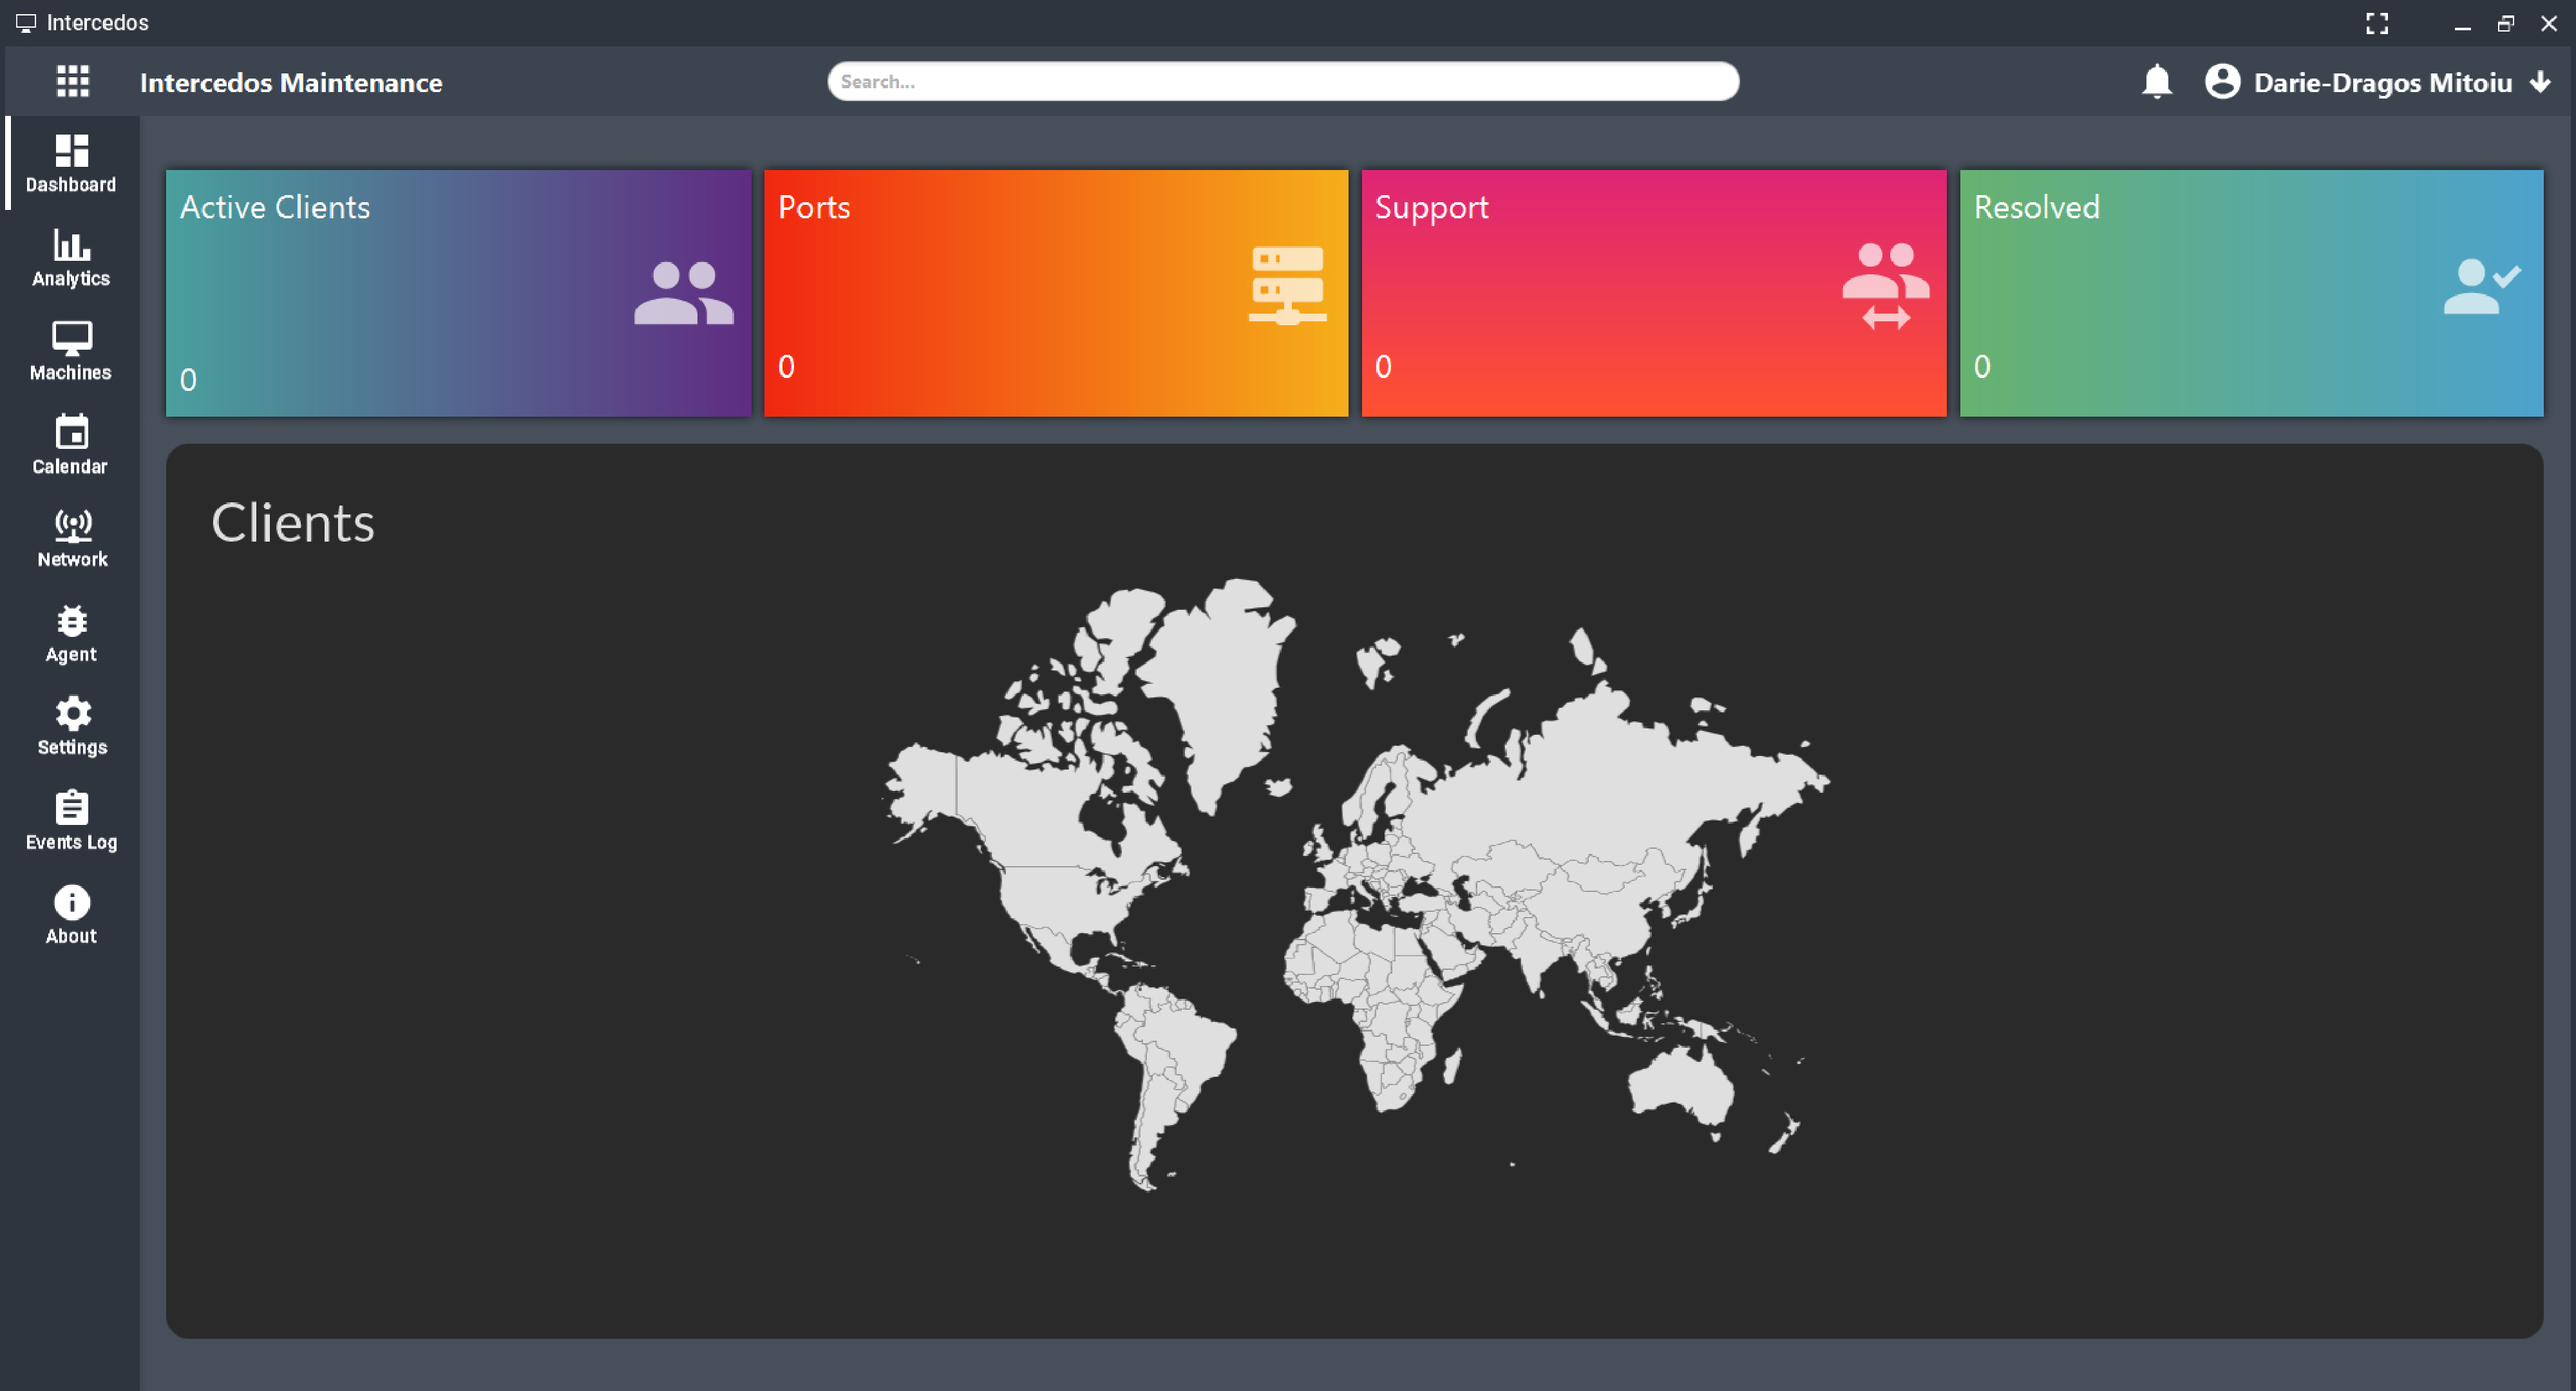
\includegraphics[width=1.0\textwidth]{images/dashboard-dark-theme.pdf}
    \captionsetup{justification=centering}
    \caption[Command and Control (C\&C) Dark Theme]{Command and Control (C\&C) Dark Theme}
    \label{fig:command-dark-theme}
\end{figure}

\newpage

\begin{figure}[h]
    \centering
    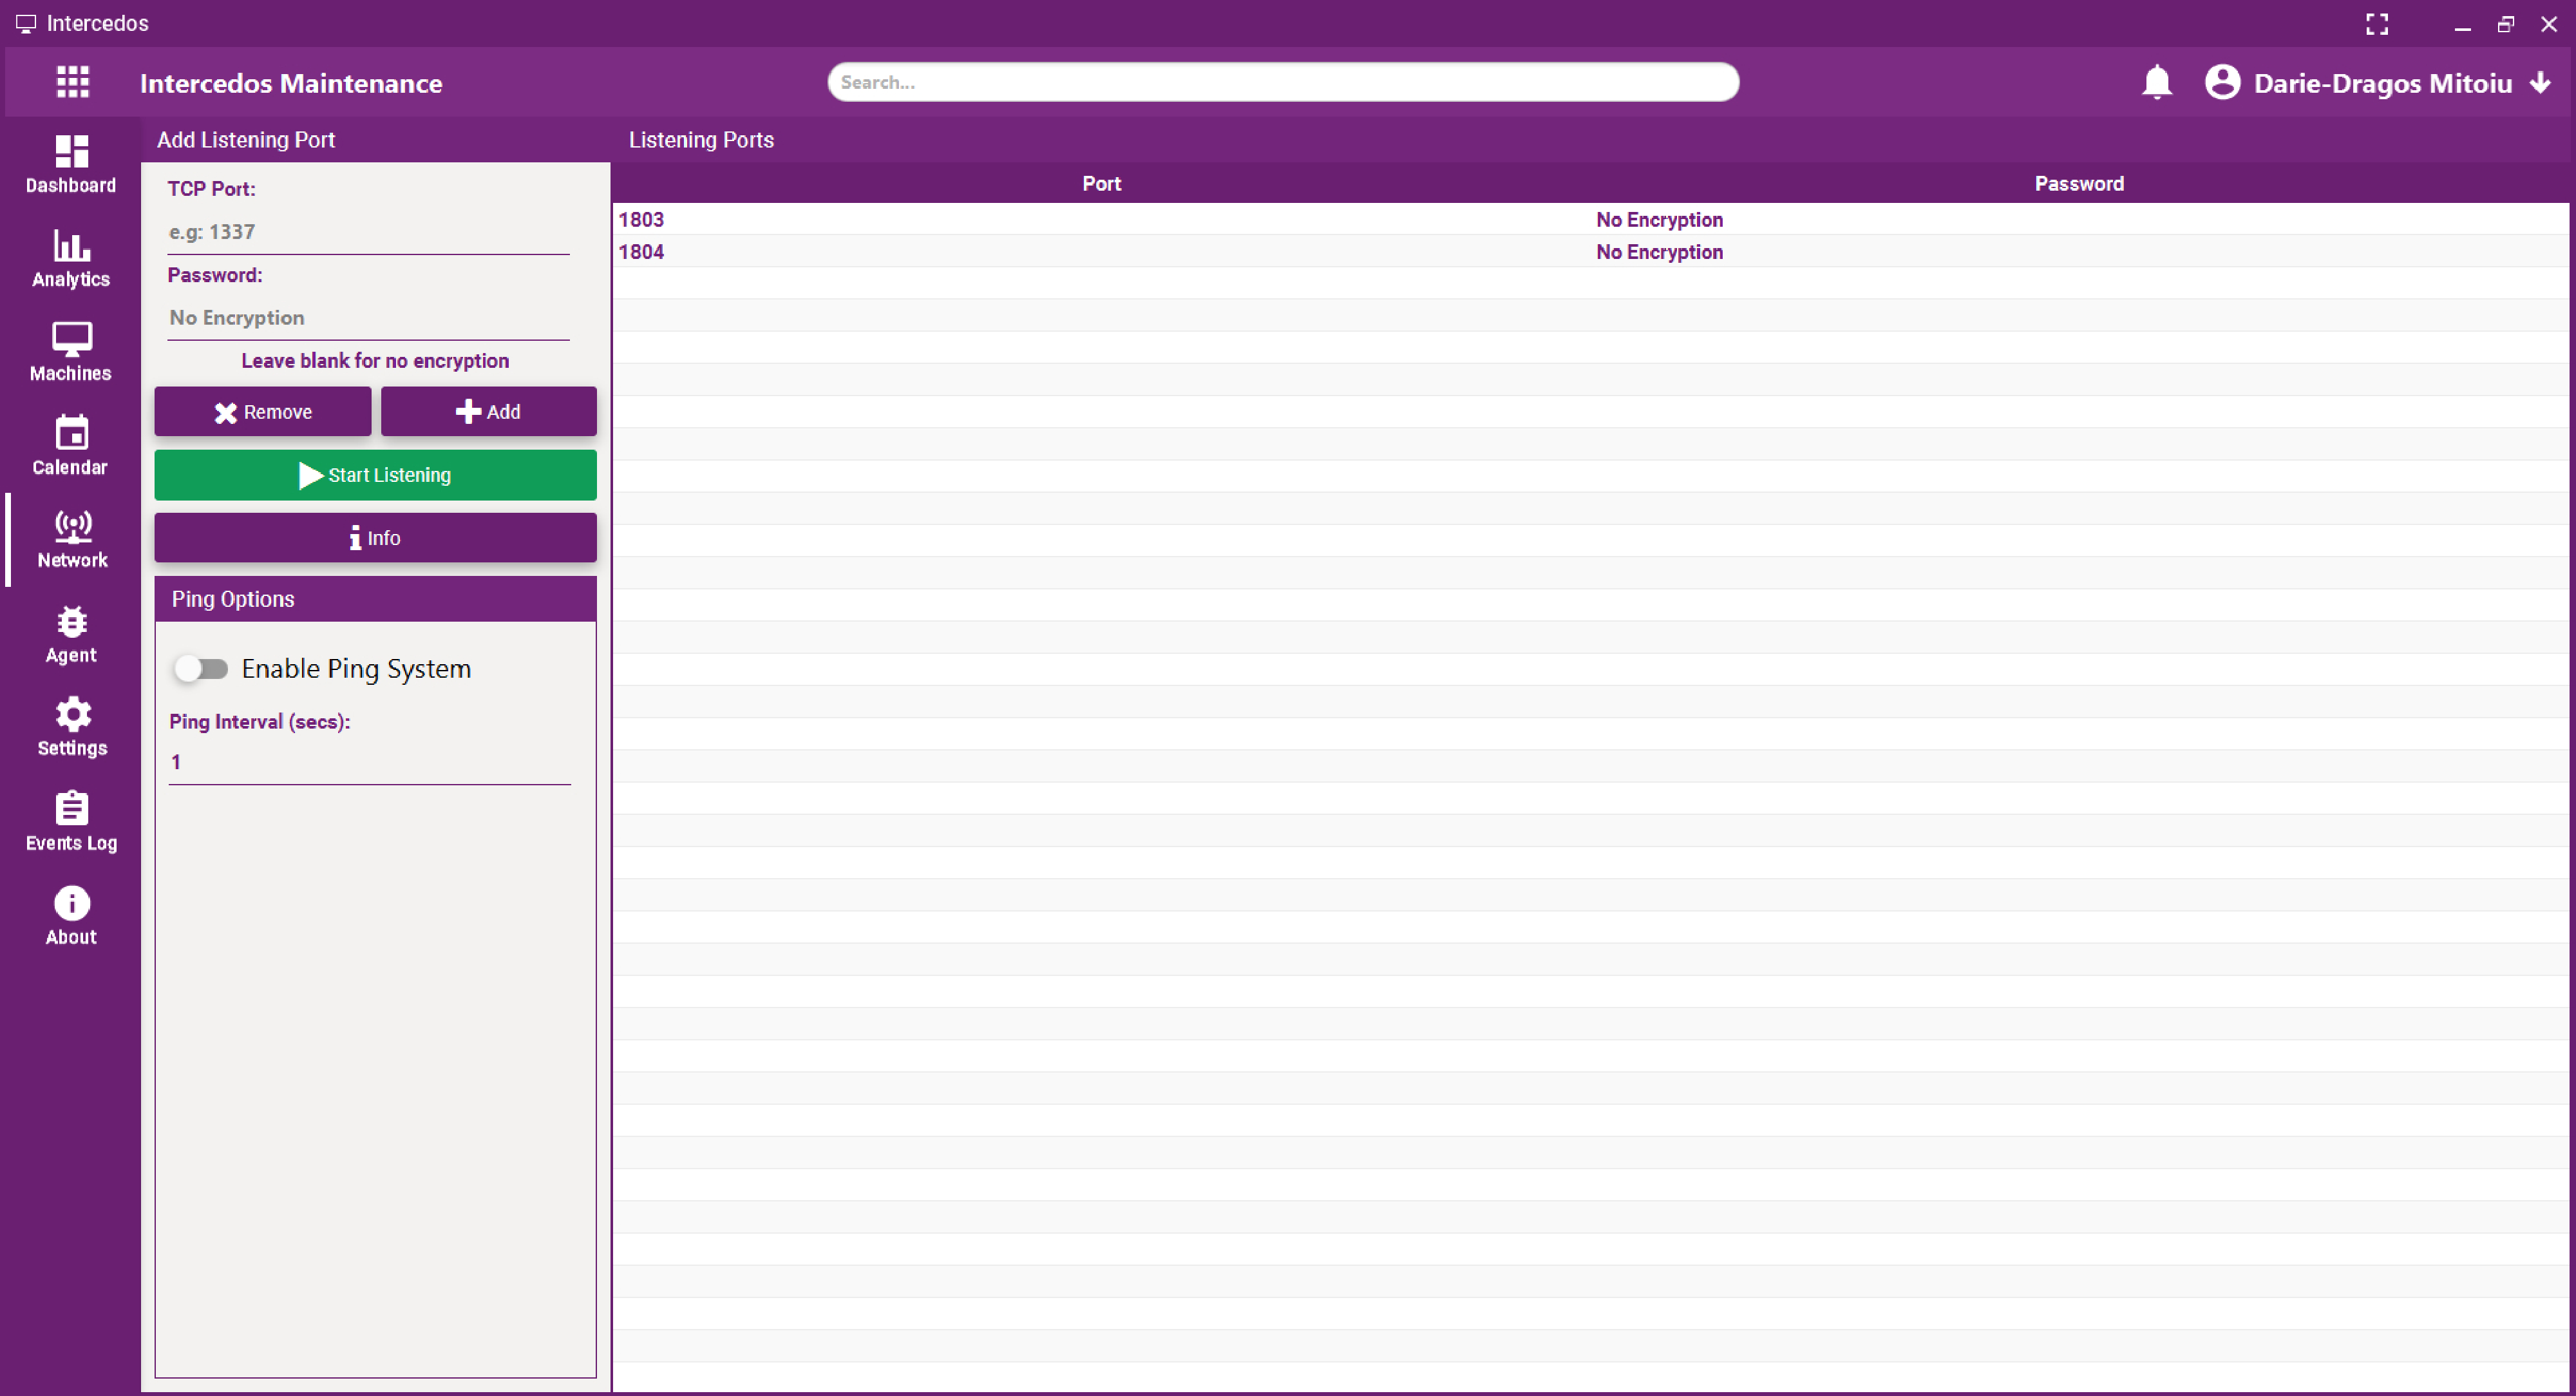
\includegraphics[width=1.0\textwidth]{images/network-panel-light-theme.pdf}
    \captionsetup{justification=centering}
    \caption[Command and Control (C\&C) Network Panel]{Command and Control (C\&C) Network Panel}
    \label{fig:command-network}
\end{figure}

\begin{figure}[h]
    \centering
    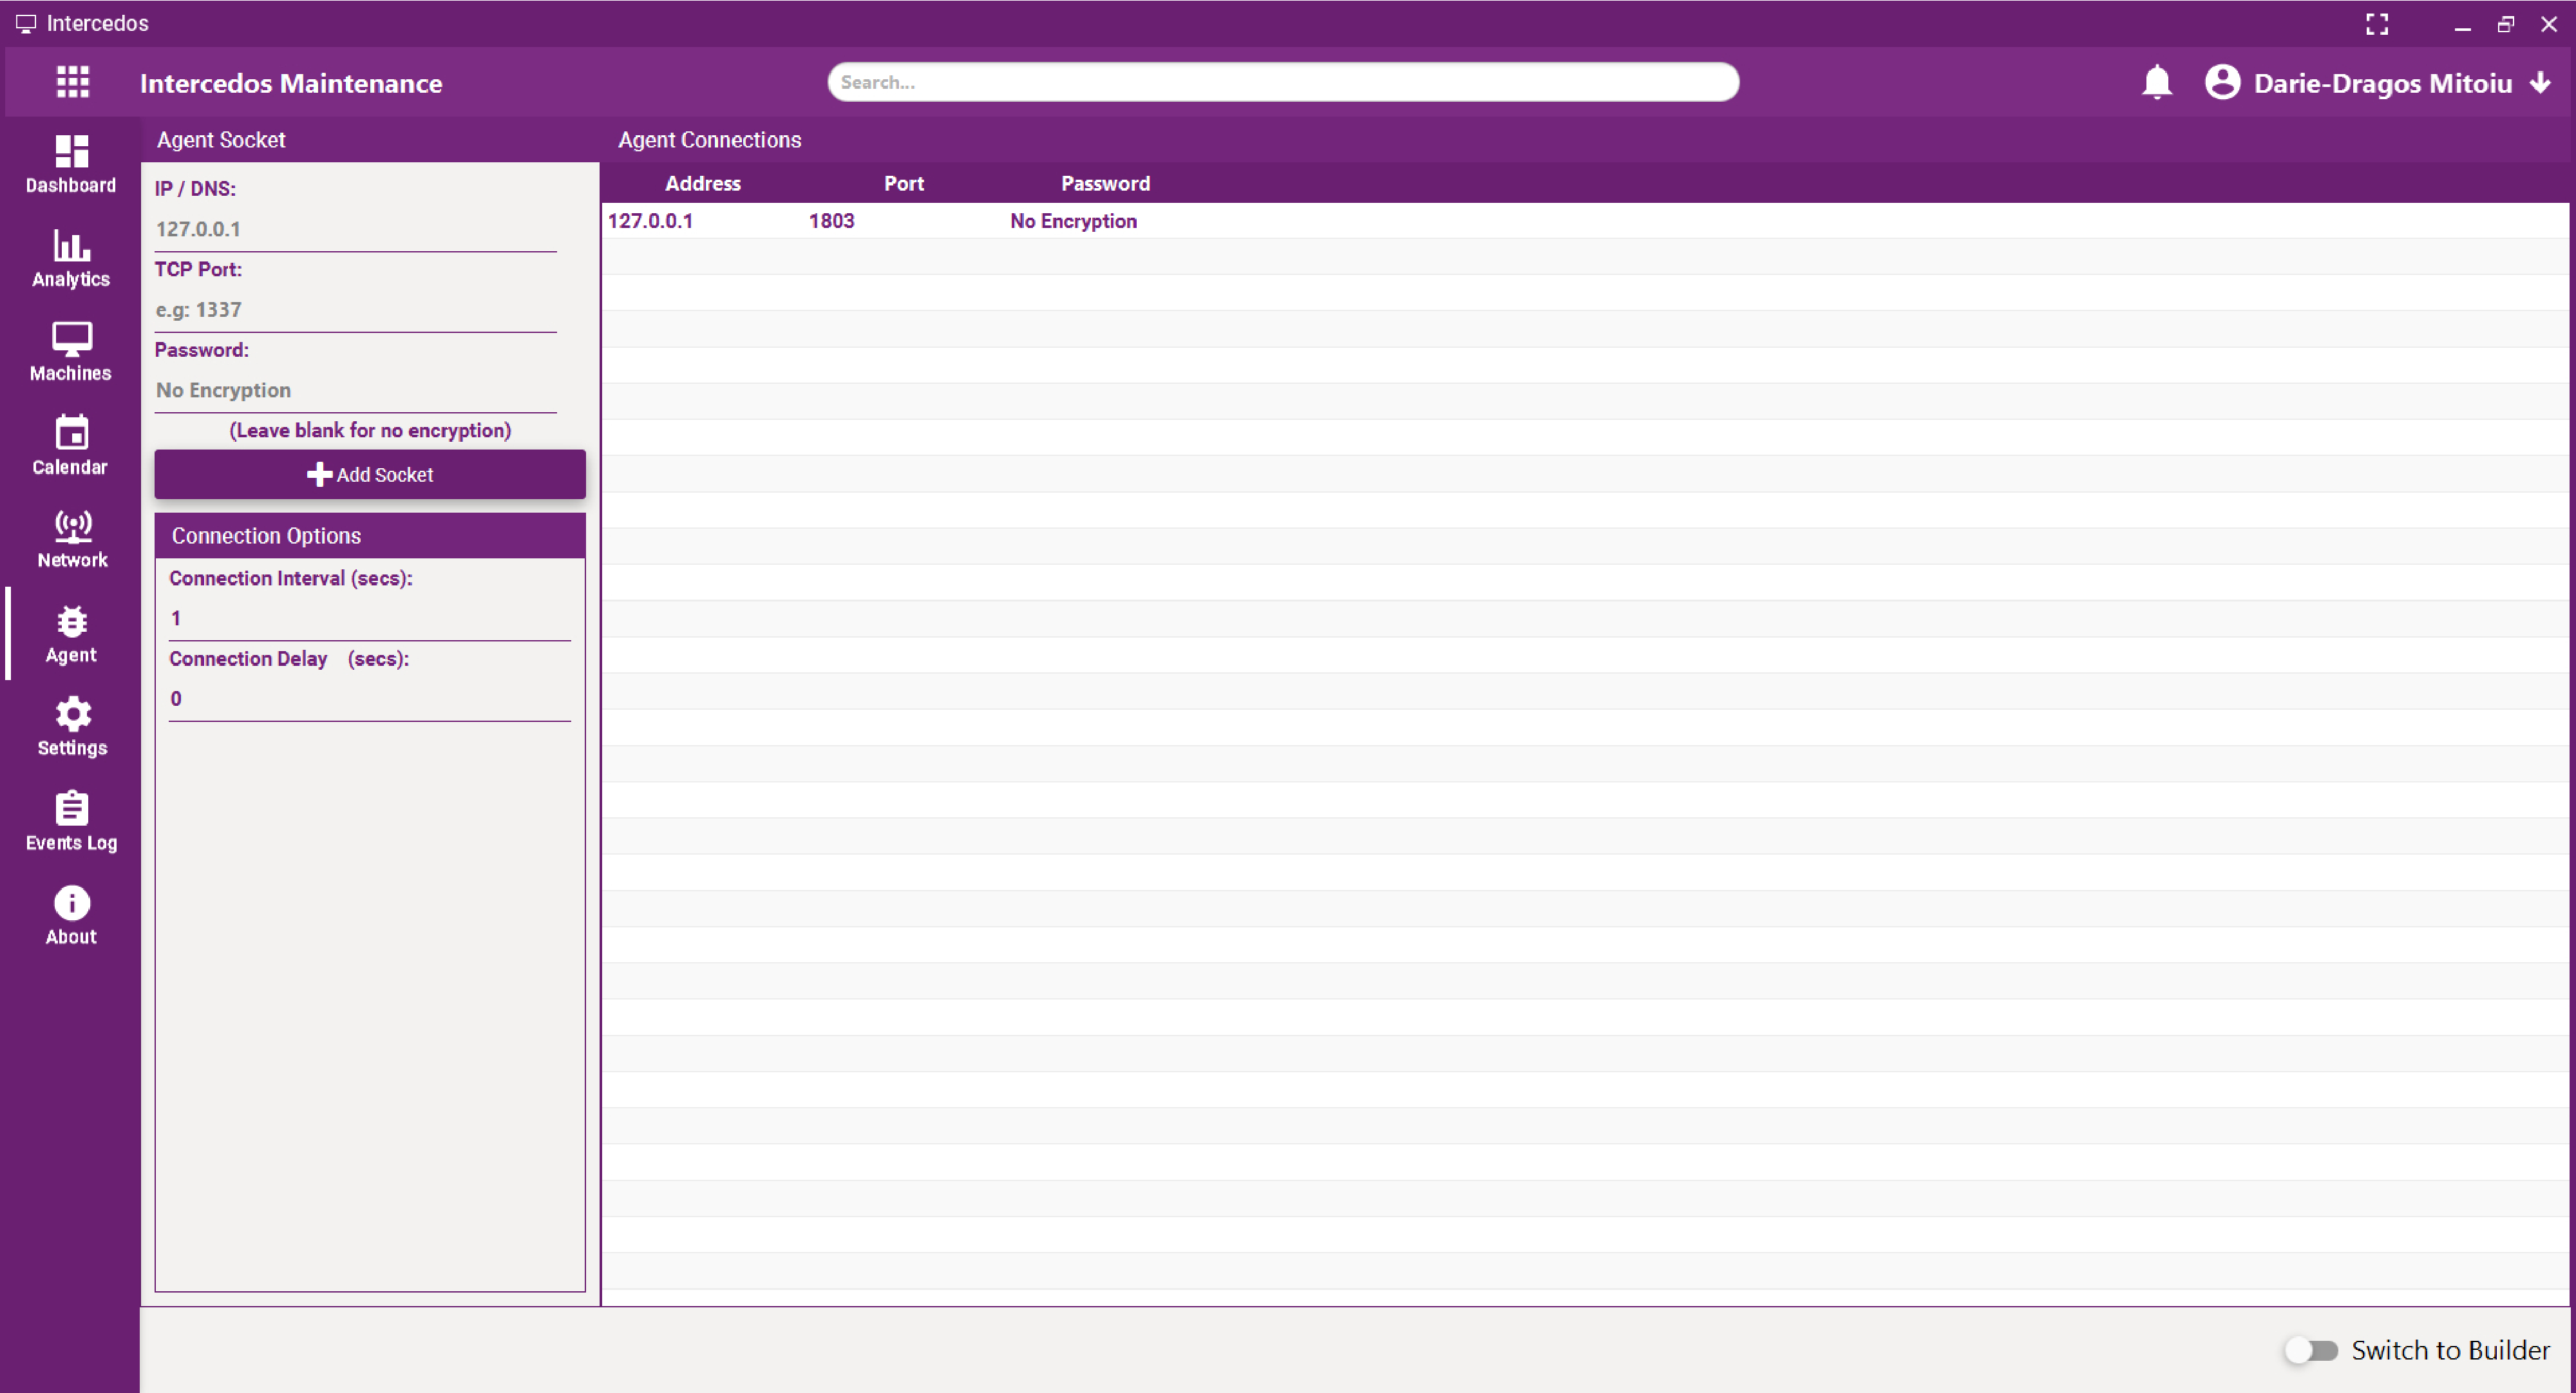
\includegraphics[width=1.0\textwidth]{images/agent-panel-light-theme.pdf}
    \captionsetup{justification=centering}
    \caption[Command and Control (C\&C) Agent Panel]{Command and Control (C\&C) Agent Panel}
    \label{fig:command-agent}
\end{figure}

\newpage

\subsubsection{MigLayout}

The creation of rich and complex Graphical User Interfaces can be a tedious and time
consuming process. Both Swing and JavaFX Interface Frameworks present build-in containers
or layouts which will allow the creation of the graphical user interface either by writing
Java instructions or just by using a third-party tool such as Scene Builder for JavaFX
which will generate some FXML based on some interactions with a graphical
user interface tool. However, this process is not efficient enough as even with the help of
third-party tool such as Scene Builder in the case of JavaFX as there will still
be limitations in the graphical user interface created without some additions of multiple
types of layouts to create the desired result, as the build-in layouts lack the capabilities to create
rich and complex layouts using just a single type of layout. This problem it is addressed
by the third-party layout called MigLayout which it is a grid based type of layout designed
specifically to avoid the utilisation of multiple types of containers or layouts to achieve
the desired result, the MigLayout container can be used for both Swing Interface Framework
and the JavaFX Interface Framework with the same syntax achieving the same result.
The \acrfull{cc} Server Application has been built using mostly the MigLayout for the
creation of the application's containers, this layouts has allowed the acceleration of
the development of the application in a significant way due to the numerous features
randing from the creation of responsive Graphical User Interfaces to the ability to
add or remove graphical components at need during run-time of the application.
It must be noted that each Graphical User Interface, Swing or JavaFX, will require
a different type of MigLayout dependency in order to function properly,
the interoperability will still be possible with the use of the MigLayout between
the Swing Framework and the JavaFX Framework, yet the appropriate Interface Nodes
must be used.

\subsection{Controller}

The controller of the \acrfull{cc} Server application will have the role to act as an
intermediary between the Graphical User Interface (JavaFX) and the models of the
application. As composition, the controller will consists of a package called
authentication, database, network, messages, build and logger. The authentication
package will contain Java Classes related to the Amazon Cognito Authentication Database
for actions such as user registration, user log in and password recovery. The database
package will contain Java Classes related to the local SQLite Database which will hold
specific ports which can be opened by the \acrfull{cc} Server. The network package will
hold packages related to the networking programming aspect of the application such as
the TCP Server with the associated Object Input Stream and Object Output Stream for data
transmission. The messages package will contain Java Classes related to specific Java
Classes which will behave as network packets as all classes in this package implement the
Serializable Java Interface. The Build package will contain code related to the creation
of the agent application. The logger package will contain Java Classes related to the
appending of informative log events which will be added to the Graphical User Interface.

\newpage
\subsubsection{Agent Configuration}

\begin{lstlisting}[language=Java, label={lst:agent-constants}, style=Oracle, columns=fullflexible,
caption=Agent (Client-Side) Constants Class,
captionpos=b]
public class Constants {
    public final static String SERVER_ADDRESS = "127.0.0.1";
    public final static int SERVER_PORT = 1337;
    public final static String T_CLASS = "/client/ClientApplication.class";
    public final static String T_METHOD = "main";
    public final static String T_DESCRIPTOR = "([Ljava/lang/String;)V";
}
\end{lstlisting}

\begin{lstlisting}[language=Java, style=Oracle, columns=fullflexible,
caption=Agent (Client-Side) Java Bytecode Manipulation,
captionpos=b]
ClassVisitor classVisitor = new ClassVisitor(ASM5, cw) {
    @Override
    public FieldVisitor visitField(int access,String name,String descriptor,
                                   String signature,Object value) {
        if(name.equals("SERVER_ADDRESS"))
            value = serverAddress;
        if(name.equals("SERVER_PORT"))
            value = serverPort;
        return super.visitField(access,name,descriptor,signature,value);
    }
    @Override
    public MethodVisitor visitMethod(int access,String name,String desc,
                                     String signature,String[] exceptions) {
        MethodVisitor mv = super.visitMethod(
                access, name, desc, signature, exceptions);
        if(name.equals(Constants.T_METHOD)
                && desc.equals(Constants.T_DESCRIPTOR)) {
            return new MethodVisitor(Opcodes.ASM5, mv) {
                @Override
                public void visitLdcInsn(Object address) {
                    if(Constants.SERVER_ADDRESS.equals(address))
                        address = serverAddress;
                    super.visitLdcInsn(cst);
                }
                @Override
                public void visitIntInsn(int i, int port) {
                    if(Constants.SERVER_PORT == port)
                        port = serverPort;
                    super.visitIntInsn(i, port);
                }
            };
        }
        return mv;
    }
};
\end{lstlisting}

\newpage

\begin{lstlisting}[language=Java, label={lst:agent-configuration}, style=Oracle, columns=fullflexible,
caption=Agent (Client-Side) Configuration Creation,
captionpos=b]
private static byte[] createConfiguration(String serverAddress,
                                          int serverPort) {
    log.info("Generating agent configuration...");
    String modifyClass = Constants.T_CLASS;
    InputStream path = Constants.class.getResourceAsStream(modifyClass);
    ClassReader cr = new ClassReader(path);
    ClassWriter cw = new ClassWriter(cr,0);
    cr.accept(classVisitor, 0);
    cw.visitEnd();
    return cw.toByteArray();
}
\end{lstlisting}

The \acrfull{cc} Server Application will present a feature which can be considered to be at
the core of the application when it comes to the Hard-Disk Drive \acrfull{smart} indicators
data retrieval, this feature is the agent creation which it is one of the most complex
features of the application as it involves the manipulation of Java Bytecode in order
ratify a series of instructions due to the dynamic configuration of the agent by the
user using the Graphical User Interface. In the figure \ref{lst:agent-constants}
it can be observed a list of static constants which have the role to hold the agent
configuration and the Java Class Manipulation Key values. The constants are placed
into a class called "Constants" which will allow the access to these values by calling
the "Constants" class though the project. The constants called "SERVER\_ADDRESS" refers
to the IP address which will be given to the agent application dynamically by the \acrfull{cc}
application in order to establish a connection, usually this address would be the same
address of the machine which will execute or run the \acrfull{cc} Server Application.
The constant called "SERVER\_PORT" refers to the port given to the agent application
dynamically by the \acrfull{cc} application to complement the previous IP address.
The "Constants" Class also contains a series of constants which are aiming at the
Java Bytecode manipulation of a specific Java Class, these constants use the prefix letter
"T" which stands for transform, the contant class called "T\_CLASS" specifies the class
to be modified at run-time, the constant called "T\_METHOD" specifies the method which
has to be modified at run-time and last but not the least the constant called
"T\_DESCRIPTOR" it is used in order to specify the type of the method which will be
modified which in this case it is a String type. The transform constants will be used
in association with the ClassVisitor of the ASM Java Bytecode Manipulation Library from
France Telecom. The ClassVisitor object created will perform all the modifications required
based on the transform constants. Once the classVisitor object it is created then the
generation of the agent configuration can happen as it can be seen in
the \ref{lst:agent-configuration} and the newly created class it is
returned from the method as a byte array which will be used at
the creation of the Java Archive (.jar).
The constants and variables used in the \ref{lst:agent-constants} code list and
\ref{lst:agent-configuration} code list have been adapted in order to fit in the
paper of the document, to explain the shorthands used in the naming of the
constants.

\newpage

\subsubsection{Agent Builder}

\begin{lstlisting}[language=Java, style=Oracle, columns=fullflexible,
caption=Agent (Client-Side) Builder,
captionpos=b]
private static void jarBuilder(File input, File output){
    try{
        JarFile jarFile = new JarFile(input);
        String className = ClientApplication.class.getName();
        String clientClass = "client/controller/network/Constants.class";
        Manifest manifest = new Manifest(jarFile.getManifest());
        manifest.getMainAttributes().putValue("Main-Class", className);

        FileOutputStream fileOutStream;
        JarOutputStream jarOutStream;
        fileOutStream = new FileOutputStream(output);
        jarOutSream = new JarOutputStream(fileOutSream, manifest);

        Enumeration<JarEntry> entries = jarFile.entries();
        Host host = (Host) connectionsTable.getItems().get(0);
        byte[] constants = createConfiguration(host.getAddress(),
                                               host.getPort());
        while(entries.hasMoreElements()){
            JarEntry jarEntry = entries.nextElement();
            if(!jarEntry.getName().equals("META-INF/MANIFEST.MF")){
                if(jarEntry.getName().equals(clientClass)){
                    ZipEntry conEntry = new ZipEntry(jarEntry.getName());
                    constantsEntry.setSize(constants.length);
                    jarOutputStream.putNextEntry(conEntry);
                } else {
                    jarOutputStream.putNextEntry(jarEntry);
                }
                if(!jarEntry.isDirectory()){
                    if(jarEntry.getName().equals(clientCLass)){
                        jarOutputStream.write(constants);
                    } else {
                        jarOutputStream.write(IOUtils.
                        toByteArray(jarFile.getInputStream(jarEntry)));
                    }
                }
                jarOutputStream.closeEntry();
            }
        }
        jarFile.close();
        jarOutputStream.close();
    } catch (IOException e){
        e.printStackTrace();
    }
}
\end{lstlisting}

\newpage

\subsection{Authentication System}

The \acrfull{cc} Server Application uses the Amazon Cognito Database in order to grant
access to the main features of the application. The Amazon Cognito Database provides
authentication, authorization and user management for web application, mobile applications
and desktop application. This type of database will allow the user to log in using
their email and password. The two main component of the Amazon Cognito Database are
the User Pools and the Identity pools, the User Pools can be considered as user
directories which can provide registration options for the application, while the
identity pools allow access to other Amazon Services. The Amazon Cognito Database
will require the following fields to be provided by the user in order to allow
the account creation: Given Name, Family Name, Email and Password.

\subsection{Local Database}

The \acrfull{cc} Server Application uses two main SQLite tables, these tables are
the "connections" table and the "banlist" table. The connections table will contain
the ports associated with their passwords which can be seen in the figure
\ref{fig:command-network}. The table called "banlist" does not present any implemented
features in the current version of the \acrfull{cc} Server. However, the "banlist" table
will be used to block specific agent connections at need by using their IP address.

\subsubsection{SQLite Structure}

\begin{lstlisting}[language=SQL, style=Oracle, columns=fullflexible,
       caption=Command \& Control (C\&C) SQLite Tables,
       captionpos=b]
CREATE TABLE connections(
    port integer(10),
    password varchar(255)
);

CREATE TABLE banlist(
    ip varchar(255),
    reason varchar(255)
);
\end{lstlisting}

\begin{lstlisting}[language=SQL, style=Oracle, columns=fullflexible,
caption=Agent (Client-Side) SQLite Tables,
captionpos=b]
CREATE TABLE servers(
    address varchar(255),
    port integer(10),
    description varchar(255),
    password varchar(255)
);
\end{lstlisting}

\subsection{Networking}

\subsubsection{Transmission Control Protocol (TCP)}

The term \acrfull{tcp} refers to the standard method of how to establish and maintain
a network connection or conversation though which applicaions or programs can send
and receive data. The \acrfull{tcp} it is associated with the Internet Protocol (IP)
which defines how computer systems can send packets of data between each other (Lutkevich 2020).

\subsubsection{User Datagram Protocol (UDP)}

The term \acrfull{udp} refers to a protocol of communications that is primarily used for
establishment of connections which are categorised as low-latency and loss-tolerating
connections between applications or programs over the internet. This approach it will
accelerate the transmission of data by enabling the transfer of data before an
agreemenet or hand-shake with the receiving party (Rosencrance and Lawton and Moozakis 2020).

\subsubsection{Hard-Disk Drive S.M.A.R.T Attribute Class}

\begin{lstlisting}[language=Java, style=Oracle, columns=fullflexible,
caption=Hard-Disk Drive S.M.A.R.T Attribute Class,
captionpos=b]
public class DiskAttribute implements Serializable {
    private int id;
    private String name;
    private String flag;
    private int value;
    private int worst;
    private int thresh;
    private String type;
    private String updated;
    private String failed;
    private String raw;

    public DiskAttribute(String name, String flag, int value, int worst,
                         int thresh, String type, String updated,
                         String failed, String raw){
        this.name = name;
        this.flag = flag;
        this.value = value;
        this.worst = worst;
        this.thresh = thresh;
        this.type = type;
        this.updated = updated;
        this.failed = failed;
        this.raw = raw;
    }
}
\end{lstlisting}

\newpage

\section{Agent (Client-Side)}

The Agent (Client-Side) Application it is composed of two main components, these two components
are the controller of the application and the data models which the application is using.
The controller of the application it is split into another two components which the configuration
component and the network component.

\subsection{Controller}

The most important component of the Agent (Client-Side)
application it is the network component as it contains all the necessary tools in order to
retrieve the Hard-Disk Drive \acrfull{smart} indicators data, yet in order to do this, the
agent application must be executed as administrator with the third-party application called
Smartmontools installed on the machine which will run the application.

\subsection{Networking}

The Agent (Client-Side) Application it uses the \acrfull{tcp} in order to communicate with the \acrfull{cc} Server
Application, this is due to the ensurance of the packets tranmission over the network which the \acrfull{tcp}
provides, this aspect is not present for the \acrfull{udp} alternative.

\section{Security}

When it comes to the security of the \acrfull{cc} Server Application and the Agent (Client-Side) Application,
the specifications and design have considered the security concerns related to the transmission of Hard-Disk Drive
\acrfull{smart} data over the network, this consideration can be seen in the figure \ref{fig:command-network}
and figure \ref{fig:command-agent} as the "password" element implies some consideration of symmetric encryption
for the data transfer. However due to lack of time, the current versions of \acrfull{cc} Server Application and
Agent (Client-Side) Application do not present any encryption capabilities and the data is sent unencrypted over
the network.

\section{Testing}

Both \acrfull{cc} Server Application and Agent (Client-Side) have been tested using a manual testing approach, the
results can be seen in the table \ref{table:command-tests} and respectively table \ref{table:agent-tests}. The tables
mentioned do not contain any evidence of the tests, for this aspect the Demonstration of the project will evidence that.

\newpage

\section{Machine Learning}

\subsection{Hard-Disk S.M.A.R.T Indicators}

\noindent
\begin{longtable}{
|p{\dimexpr.40\linewidth-2\tabcolsep-1.3333\arrayrulewidth}% column 1
|p{\dimexpr.60\linewidth-2\tabcolsep-1.3333\arrayrulewidth}|% column 2
}
    \hline
    \centering S.M.A.R.T Attribute ID  & \centering\arraybackslash S.M.A.R.T Attribute Name    \hline
    SMART 1                               & \centering Raw Read Error Rate                     \hline
    SMART 3                               & \centering Spin Up Time                            \hline
    SMART 4                               & \centering Start Stop Count                        \hline
    SMART 5                               & \centering Reallocated Sector Count                \hline
    SMART 7                               & \centering Seek Error Rate                         \hline
    SMART 9                               & \centering Power On Hours                          \hline
    SMART 183                             & \centering Runtime Bad Block                       \hline
    SMART 184                             & \centering End-To-End Error                        \hline
    SMART 187                             & \centering Reported Uncorrectable Errors           \hline
    SMART 188                             & \centering Command Timeout                         \hline
    SMART 189                             & \centering High Fly Writes                         \hline
    SMART 190                             & \centering Temperature Difference                  \hline
    SMART 191                             & \centering G-Sense Error Rate                      \hline
    SMART 193                             & \centering Load Cycle Count                        \hline
    SMART 194                             & \centering Temperature Celsius                     \hline
    SMART 197                             & \centering Current Pending Sector                  \hline
    SMART 198                             & \centering Offline Uncorrectable                   \hline
    SMART 199                             & \centering UDMA CRC Error Count                    \hline
    SMART 200                             & \centering Multi Zone Error Rate                   \hline
    SMART 201                             & \centering Soft Read Error Rate                    \hline
    SMART 202                             & \centering Data Address Mark Errors                \hline
    SMART 203                             & \centering Run Out Cancel                          \hline
    SMART 204                             & \centering Soft ECC Correction                     \hline
    SMART 205                             & \centering Thermal Asperity Rate                   \hline
    SMART 206                             & \centering Flying Height                           \hline
    SMART 207                             & \centering Spin High Current                       \hline
\end{longtable}
\captionof{table}{SMART Attributes Names}

\newpage

\noindent
\begin{longtable}{
|p{\dimexpr.30\linewidth-2\tabcolsep-1.3333\arrayrulewidth}% column 1
|p{\dimexpr.32\linewidth-2\tabcolsep-1.3333\arrayrulewidth}% column 2
|p{\dimexpr.38\linewidth-2\tabcolsep-1.3333\arrayrulewidth}|% column 3
}
    \hline
    \centering S.M.A.R.T Attribute  & \centering Seagate ST4000DM000 & \centering\arraybackslash Hitachi HDS722020ALA330  \\ \hline
    smart\_1\_norm                               & \centering 23\%        & \centering 28\%        \hline
    smart\_1\_raw                                & \centering 2\%         & \centering 15\%        \hline
    smart\_5\_norm                               & \centering 2\%         & \centering 22\%        \hline
    smart\_5\_raw                                & \centering 19\%        & \centering 31\%        \hline
    smart\_7\_norm                               & \centering 14\%        & \centering -           \hline
    smart\_7\_raw                                & \centering 26\%        & \centering -           \hline
    smart\_183\_norm                             & \centering 0.5\%       & \centering -           \hline
    smart\_183\_raw                              & \centering 0.5\%       & \centering -           \hline
    smart\_184\_norm                             & \centering 1\%         & \centering -           \hline
    smart\_184\_raw                              & \centering 1\%         & \centering -           \hline
    smart\_187\_norm                             & \centering 21\%        & \centering -           \hline
    smart\_187\_raw                              & \centering 21\%        & \centering -           \hline
    smart\_188\_norm                             & \centering 0\%         & \centering -           \hline
    smart\_188\_raw                              & \centering 10\%        & \centering -           \hline
    smart\_189\_norm                             & \centering 1\%         & \centering -           \hline
    smart\_189\_raw                              & \centering 1\%         & \centering -           \hline
    smart\_190\_norm                             & \centering 2\%         & \centering -           \hline
    smart\_190\_raw                              & \centering 2\%         & \centering -           \hline
    smart\_193\_norm                             & \centering 10\%        & \centering -           \hline
    smart\_193\_raw                              & \centering 63\%        & \centering -           \hline
    smart\_194\_norm                             & \centering 2\%         & \centering 31\%        \hline
    smart\_194\_raw                              & \centering 2\%         & \centering 2\%         \hline
    smart\_197\_norm                             & \centering 5\%         & \centering 4\%         \hline
    smart\_197\_raw                              & \centering 27\%        & \centering 22\%        \hline
    smart\_198\_norm                             & \centering 6\%         & \centering -           \hline
    smart\_198\_raw                              & \centering 27\%        & \centering -           \hline
\end{longtable}
\captionof{table}{SMART Correlation Frequencies for Seagate and Hitachi models
(Botezatu, Giurgiu, Bogojeska and Wiesmann 2016 p. 5 table 2)}

\setlength{\parindent}{1.5em}
\subsection{BackBlaze Data}

In order to prove the viability of forecasting computer systems failure using machine learning techniques and the
Hard-Disk Drive \acrfull{smart} indicators, a series of experiments were performed using data provided by the
BackBlaze company. The Data provided it is from a signle vendor of Hard-Disk componenet which aims at the model
Seagate ST4000DM000, the data also it is relatively new as it is from the year 2017.
This specific study is aiming specifically at the machine learning algorithm
called \acrfull{svm}.

\subsection{Data Exploration}

When the exploration of the data was performed it was seen that the data file contains 142,638 records and 95 features.

\subsection{Data Pre-Processing}

Before creating the machine learning models, a series of pre-processing operations were performed, these
operations are the handling of missing values, the selection of the most relevant features and
the balance of class distribution.

\subsubsection{Features Selection}

According to Beach (2014) the most relevant Hard-Disk Drive \acrfull{smart} features are the following:

\begin{itemize}
    \item SMART 5:   Reallocated\_Sector\_Count,
    \item SMART 187: Reported\_Uncorrectable\_Errors,
    \item SMART 188: Command\_Timeout.
    \item SMART 197: Current\_Pending\_Sector\_Count.
    \item SMART 198: Offline\_Uncorrectable.
\end{itemize}

\subsection{Classification}

\noindent
\begin{longtable}{
|p{\dimexpr.35\linewidth-2\tabcolsep-1.3333\arrayrulewidth}% column 1
|p{\dimexpr.20\linewidth-2\tabcolsep-1.3333\arrayrulewidth}% column 2
|p{\dimexpr.20\linewidth-2\tabcolsep-1.3333\arrayrulewidth}% column 3
|p{\dimexpr.25\linewidth-2\tabcolsep-1.3333\arrayrulewidth}|% column 4
}
    \hline
    \centering Algorithm  & \centering F-1 Score & \centering ROC AUC   & \centering\arraybackslash Accuracy (\%)  \\ \hline
    Support Vector Machines        & \centering 0.44      & \centering 0.67      & \centering 94.56\%        \hline
    Random Forest Model            & \centering 0.50      & \centering 0.70      & \centering 95.10\%        \hline
    Logistic Regression            & \centering 0.45      & \centering 0.68      & \centering 94.61\%        \hline
    Multi-Layer Perceptron         & \centering 0.46      & \centering 0.69      & \centering 94.52\%        \hline
\end{longtable}
\captionof{table}{Best Results for each algorithm used for the experiments}



    \setlength{\parindent}{1.5em}
    \chapter{Evaluation}
    The two project components mentioned in the design and implementation chapters
- \acrfull{cc} Server Application and the Agent (Client-Side) Application - have been
successfully implemented. The networking features of both applications will allow the transfer of data between the \acrfull{cc}
and the Agent (Client-Side) application successfully, however, due to lack of resources in the form of computer systems
for data collection, the forecasting of computer systems is not present at the current stage for the \acrfull{cc}
Server Application, instead a Static Analysis was performed in the implementation chapter
in order to prove the viability of forecasting computer systems failure using the Hard-Disk Drive \acrfull{smart}
indicators.
It is important to note that due to lack of resources, time and the high level of project complexity
there was a permanent risk of project failure, yet a foundation which will allow
future development it is present and the forecasting of computer systems failure was proved and evidenced. \par
Firstly, in this chapter the two main components - \acrfull{cc} Server Application and
the Agent (Client-Side) application - of the project will be evaluated
against the functional requirements mentioned in the specifications chapter using their appropriate notes. \par
Secondly, this chapter will cover and evaluate the viability of forecasting computer systems failure
using the Hard-Disk Drive \acrfull{smart} indicators and a considerable amount of data collected to
train machine learning algorithms such as \acrfull{svms}, Logistic Regression and the Random-Forest Model. \par
Finally, this chapter will cover how possible improvements related to the - \acrfull{cc} Server Application,
Agent (Client-Side) Application and the machine learning aspect - of the project could be performed. The improvements
features which will be discussed in this chapter will concern the viability of future development for the - \acrfull{cc}
Server Application by adding the Machine Learning discoveries presented into the implementation chapter
into a viable feature which will forecast computer systems failure using the Hard-Disk Drive \acrfull{smart}
indicators.

\section{Acceptance Testing}

The term "Acceptance Testing" refers to a technique used for software testing which
is performed in order to determine whether a specific software system has met or not a series of
requirements. The role of an acceptance test it is to evaluate if the system is compliant with
the business requirements and to check if it has met the needs of the end-users (Tutorials Point 2021).

\subsection{Command and Control (C\&C)}

The \acrfull{cc} Server Application at the end of the project development cycle in the allocated time frame presents
73 functional requirements out of 86 functional requirements mentioned in the specifications chapter. It is easy to
notice that the number mentioned shows some considerable development success. However, some functional requirements
labeled as "should" and "could" have not been implemented, either from lack of available time or because a different
development approach has been taken, e.g: The machine learning aspect of the \acrfull{cc} Server Application has been
replaced with a static analysis of a BackBlaze dataset.

\subsection{Agent (Client-Side)}

The Agent (Client-Side) Application at the end of the project development cycle in the allocated time frame presents
10 functional requirements out of 12 functional requirements mentioned in the specifications chapter. It is easy to
notice that the number mentioned shows some considerable development success. However, some functional requirements
labeled as "should" have not been implemented due to lack of development time.

\subsection{Machine Learning}

The Machine Learning Aspect of the project had to be associated with the use the of the BlackBlaze Hard-Disk Drive
\acrfull{smart} data in order to prove the viability of computer systems failure predictions as there was a lack of
resources in the form of computer systems. The Support Vector Machines algorithm was used in association with the
BackBlaze dataset and an accuracy of 94\% was produced, it is safe to say that the machine learning aspect of the
project was a complete success.

\section{Improvements}

While the metrics of the Support Vector Machines algorithm are promising, the static analysis will not offer any real
world problem solving, for this reason the \acrfull{cc} Server Application must present a feature in the future which
will allow the training of machine learning models and the testing of the models on real computer systems using a Java
library such as \acrfull{smile} which will give access to the \acrfull{svm} algorithm.

    \chapter{Conclusions}
    In this chapter the core aspects presented in the background, design and implementation chapters
will be discussed. To recapitulate, this project had the ultimate goal to investigate
if the forecast of computer systems failure using the Hard-Disk Drive \acrfull{smart} indicators
it is possible and if so, to translate the discoveries into a real-world appliance.
To do this, four main objectives had to satisfied, these objectives were to
research forecasting of computer systems failure practices, to create a \acrfull{cc} Server
Application, to create an Agent (Client-Side) Application to collect the Hard-Disk Drive
\acrfull{smart} data and last but not the least to investigate the viability of forecasting
computer systems using the machine learning algorithm called \acrfull{svm}.
The four objectives mentioned have been completed successfully.

This chapter will also cover the challenges encountered during the course of the project,
alternatives approaches for the forecasting of computer systems failure, future work that can be performed for the current
project and last but not the least the auto-evaluation or the critical analysis from a
personal point of view for this project will be given.

\section{Maintenance of Computer Systems}

During the background chapter it was seen that the research area related to the
maintenance of computer systems it is a vast and complex environment, the complexity of the
computer systems being largely represented by the dynamic and unforseen runtime of the
systems, for this type of complexity the classical reactive measure which would be taken
would not suffice and because of this a different approach had to be taken which was to
forecast possible failure events of computer systems.
In the background chapter it was seen that there are multiple approaches to the forecasting
of computer systems failure, this document only covered two of those approaches, the first
approach being the use of the machine learning algorithm called \acrfull{svms} in association with the
Hard-Disk Drive \acrfull{smart} indicators and the second approach being the use of the
statistical machine learning algorithm called \acrfull{hmm} in association with a series of
hardware sensors which will allow a failure probability to be computed.

\section{Future Work}

The project can be considered a success considering the high level of complexity and the amount
of work that had to be invested into this project, as the project consists of three sub-projects,
elements which are the \acrfull{cc} Server Application, the Agent (Client-Side) Application and the Machine Learning
aspect. The three sub-project elements have been completed successfully. However, the Machine
Learning aspect of the project on its own does not present any real-world problem solving,
because of this the Machine Learning aspect of using the \acrfull{svms} algorithm in association
with the Hard-Disk Drive \acrfull{smart} indicators must be translated into a feature for the
\acrfull{cc} Server Application, this feature should allow the training of machine learning
models using existing Hard-Disk Drive \acrfull{smart} data from a single vendor of Hard-Disk
components and tested on machines which use the same vendor, the use of single vendor of
Hard-Disk components it is important in order to have accurate predictions. \par
In addition to the Machine Learning feature for the \acrfull{cc} Server Application, the addition of a
native agent application for Windows type of Operating System must be implemented in the
future as the current Java Archive (.jar) Agent Application will require the installation
of the Java Runtime Environment 8 on the machine which will execute the program.

\section{Auto-Evaluation}

Considering the level of project complexity, the time frame allocated and the effort put
to complete the project, I feel satisfied with the final result and how the project was
managed during the course of the whole process. I believe that I worked to the best of my
ability at the current stage and I made use of the available time in the best possible
way. The design and implementation phases have required more time than the research part
of the project due to the iteration processes which were used in order to reach the final
result. \par
When it comes to the most difficult aspect of the project, each stage had it's own specific
challenges but for me the most difficult stage of the project was the design phase which
had to be looked into multiple times due to the inability to find the right design from the
start. \par
This project was driven by the passion for network programming, at the start of the project
the best method of learning this branch was to create a reactive maintenance tool for
computer systems, even though the final product does not present any reactive maintenance
features and it aims at a predictive method when it comes to the failure of computer
systems, the main motivation of conducting the project was that in the future the product
could present both reactive maintenance features and predictive ones using different machines learning
algorithms.

    \appendix
    \chapter{Command and Control (C\&C) Tests}

\noindent
\begin{longtable}{
|p{\dimexpr.5\linewidth-2\tabcolsep-1.3333\arrayrulewidth}% column 1
|p{\dimexpr.25\linewidth-2\tabcolsep-1.3333\arrayrulewidth}% column 2
|p{\dimexpr.25\linewidth-2\tabcolsep-1.3333\arrayrulewidth}|% column 3
}
    \hline
    \centering Requirement     & \centering Status     & \centering\arraybackslash Notes     \\ \hline
    The Desktop Application must validate the
    user input &                                       \centering Implemented        & Not Applicable         \\ \hline

    The validation of the user input must be performed
    for the TCP Listening ports when records will be
    added to the local database
                                                       & \centering Implemented        & Not Applicable         \\ \hline
    The validation of the user input must be performed
    for the IP or DNS address when records will be
    added to the local database.                       & \centering Implemented        & Not Applicable         \\ \hline
    The Desktop Application should allow the creation of client application in the form of a Java Archive
    (.jar) which will have the role to connect to a specific IP address and port specified by the user,
                                                       & \centering Implemented        & Not Applicable         \\ \hline
    The Java Archive (.jar) should be created at a file location on the storage system specified
    by the user,
                                                       & \centering Implemented         & Not Applicable         \\ \hline
    The Desktop Application must save the preferences of the application in an XML
    (Extensible Markup Language) file
                                                       & \centering Implemented         & Not Applicable         \\ \hline
    The preferences of the application must be saved using the Java Architecture for XML Binding (JAXB),
                                                       & \centering Implemented         & Not Applicable         \\ \hline
    The preferences file must contain a boolean variable related to the theme of the application,
    the value being True for the light theme and False for the dark theme.
                                                       & \centering Implemented         & Not Applicable         \\ \hline
    The Desktop Application must use the Client-Server Network Architecture,
                                                       & \centering Implemented         & Not Applicable         \\ \hline
    The Desktop Application must use the Transmission Control Protocol (TCP) for data transfer,
                                                       & \centering Implemented         & Not Applicable         \\ \hline
    The Desktop Application must allow the establishment of connections from clients or agents on the
    current machine's address and on specific ports defined by the user,
                                                       & \centering Implemented         & Not Applicable         \\ \hline
    The Desktop Application must be able to stop the establishment of connections from clients or agents
    on the current machine's address and on the specific ports defined by the user previously,
                                                       & \centering Implemented         & Not Applicable         \\ \hline
    The Desktop Application must be able to receive packets from the clients or agents connected to the server,
                                                       & \centering Implemented         & Not Applicable         \\ \hline
    The Desktop Application must be able to send packets to the clients or agents connected to the server,
                                                       & \centering Implemented         & Not Applicable         \\ \hline
    The Desktop Application must maintain the connection between the server and clients,
                                                       & \centering Implemented         & Not Applicable         \\ \hline
    The Desktop Application should allow the clients to reconnect to the server if the connection will be lost.
                                                       & \centering Not Implemented     & Not Applicable     \\ \hline
    The Desktop Application should use symmetric or asymmetric encryption for the transfer of
    data between the clients and server.
                                                       & \centering Not Implemented     & Not Applicable     \\ \hline
    The Desktop Application must present a Local Database created using SQLite.
                                                       & \centering Implemented         & Not Applicable     \\ \hline
    The local database must allow the creation of a table for listening ports called connections,
                                                       & \centering Implemented         & Not Applicable     \\ \hline
    The local database must allow the addition of records in the form of listening ports to a SQLite
    table called connections,
                                                       & \centering Implemented         & Not Applicable     \\ \hline
    The local database must allow the deletion of records in the form of listening ports from the SQLite
    table called connections.
                                                       & \centering Implemented         & Not Applicable     \\ \hline
    The local database could allow the modification of records for the listening ports added to the
    SQLite table called connections.
                                                       & \centering Not Implemented     & Not Applicable     \\ \hline
    The Desktop Application must use an AWS Cognito Authentication System
                                                       & \centering Implemented     & Not Applicable     \\ \hline
    The Authentication System must allow the user to Log In using an email address and a password,
                                                       & \centering Implemented     & Not Applicable     \\ \hline
    The Authentication System must allow the user to register using an email address, a password,
    their full name and a security code,
                                                       & \centering Implemented     & Not Applicable     \\ \hline
    The Authentication System must allow the user to register only if the input provided for the email
    address matches the format provided is valid, the full name does not contain numbers or special
    characters, the password consists of an upper case letter, a lower case letter, a number and a
    special character.
                                                       & \centering Implemented     & Not Applicable     \\ \hline
    The Authentication System could allow the user to reset their password by using their email address,
                                                       & \centering Not Implemented     & Not Applicable     \\ \hline
    The Authentication System must allow only genuine users to access the main application.
                                                       & \centering Implemented     & Not Applicable     \\ \hline
    The desktop application should use the machine learning algorithm called Support Vector Machines (SVM)
    in order to perform a classification of the Hard-Disk S.M.A.R.T (Self-Monitoring, Analysis and Reporting
    Technology) indicators collected data from the machines which will be monitored using the Java Archive
    (.jar) clients or agents and provide predictions related to hard-disk failure.
                                                       & \centering Partially Implemented     & Not Applicable \\ \hline
    The Hard-Disk S.M.A.R.T indicators data should be collected from the clients machines and saved into
    a Comma-separated values (.csv) file.
                                                       & \centering Implemented     & Not Applicable     \\ \hline
    The Hard-Disk S.M.A.R.T indicators data should be explored before any pre-processing operations,
                                                       & \centering Not Implemented     & Not Applicable  \\ \hline
    The collected data should be pre-processed before creating a Support Vector Machines (SVM) model by
    verifying the file for any missing values,
                                                       & \centering Not Implemented     & Not Applicable   \\ \hline
    The collected data should be pre-processed before creating a Support Vector Machines (SVM) model by
    verifying the data if normalisation can be applied,
                                                       & \centering Not Implemented     & Not Applicable   \\ \hline
    The collected data should be used for training a Support Vector Machines (SVM) model in order to
    provide predictions related to hard-disk failures.
                                                       & \centering Not Implemented     & Not Applicable   \\ \hline
    The Support Vector Machines (SVM) model should be trained using multiple C parameter values and
    multiple Gamma parameter values in order to get the best results.
                                                       & \centering Not Implemented     & Not Applicable   \\ \hline
    The trained Support Vector Machines (SVM) model should be tested on a sample of Hard-Disks
    S.M.A.R.T indicators data in order to evaluate the accuracy and error rate of the model.
                                                       & \centering Not Implemented     & Not Applicable   \\ \hline
    The Graphical User Interface could present a Window for the Authentication Process,
                                                       & \centering Implemented     & Not Applicable   \\ \hline
    The Window could present a button to Log In into the main application,
                                                       & \centering Implemented     & Not Applicable   \\ \hline
    The Window could present a button to register into the system,
                                                       & \centering Implemented     & Not Applicable   \\ \hline
    The Graphical User Interface could present a Window for the Terms of Service informative process which
    will inform the user of the legal and ethical aspect of using the application,
                                                       & \centering Implemented     & Not Applicable   \\ \hline
    The Window could present a button to visualise the full terms of service,
                                                       & \centering Implemented     & Not Applicable   \\ \hline
    The Window could present a button for declining the terms of service,
                                                       & \centering Implemented     & Not Applicable   \\ \hline
    The Window could present a button for accepting the terms of service,
                                                       & \centering Implemented     & Not Applicable   \\ \hline
    The Graphical User Interface could present a Window for the Main features of the application which
    will be available once the authentication process will be completed,
                                                       & \centering Implemented     & Not Applicable   \\ \hline
    The Graphical User Interface could present a welcome message with the user's full name once the
    authentication process will be completed,
                                                       & \centering Implemented     & Not Applicable   \\ \hline
    The Graphical User Interface could present a panel for general information called Dashboard for the main
    Window of the application,
                                                       & \centering Implemented     & Not Applicable   \\ \hline
    The general information panel could present a widget that shows the number of clients
    connected to the server for the current application session,
                                                       & \centering Implemented     & Not Applicable   \\ \hline
    The general information panel could present a widget that shows the number of ports opened
    by the application for the current application session,
                                                       & \centering Implemented     & Not Applicable   \\ \hline
    The general information panel could present a widget that shows the number of clients connected
    to the server that may require maintenance assistance for the current application session,
                                                       & \centering Implemented     & Not Applicable   \\ \hline
    The general information panel could present a widget that shows the number of clients connected
    to the server with resolved maintenance problems for the current application session.
                                                       & \centering Implemented     & Not Applicable   \\ \hline
    The general information panel could present a widget that shows the activity of the application
    for a week time when considering the number clients connected, open ports, maintenance assistance
    and resolved issues.
                                                       & \centering Not Implemented     & Not Applicable   \\ \hline
    The general information panel could present a widget that shows the number of causes of maintenance
    the current application session.
                                                       & \centering Not Implemented     & Not Applicable   \\ \hline
    The general information panel could present a widget that shows the number of maintenance
    notifications classified as critical, warning and informative for the current application session.
                                                       & \centering Not Implemented     & Not Applicable   \\ \hline
    The Graphical User Interface could present a panel for data analysis called Analytics for the main
    Window of the application,
                                                       & \centering Implemented     & Not Applicable   \\ \hline
    The data analysis panel could present an area chart for the collection of Hard-Disk S.M.A.R.T data
    over a week time period,
                                                       & \centering Implemented     & Not Applicable   \\ \hline
    The data analysis panel could present a table for maintenance or failure events sent by the clients
    machines with columns named as Time, Level, Event, Platform, Architecture, Computer Name, Host and
    Port.
                                                       & \centering Implemented     & Not Applicable   \\ \hline
    The Graphical User Interface could present a panel for remote execution of instructions called Machines
    for the main Window of the application,
                                                       & \centering Implemented     & Not Applicable   \\ \hline
    The remote execution of instructions panel could present a table containing the current clients
    connected to the server in the form of table records with columns named as Platform, Architecture
    Computer Name, Host, Port, Payload and Action.
                                                       & \centering Implemented     & Not Applicable   \\ \hline
    The Graphical User Interface could present a panel for past and scheduled maintenance events
    called Calendar for the main Window of the application,
                                                       & \centering Implemented     & Not Applicable   \\ \hline
    The scheduled maintenance events panel could contain a calendar view created using the user
    interface java framework called CalendarFX.
                                                       & \centering Implemented     & Not Applicable   \\ \hline
    The Graphical User Interface could present a panel for the establishment of connections called Network
    for the main Window of the application,
                                                       & \centering Implemented     & Not Applicable   \\ \hline
    The establishment of clients connections panel could present a label called "TCP Port",
                                                       & \centering Implemented     & Not Applicable   \\ \hline
    The establishment of clients connections panel could present a text field for the
    TCP Port information,
                                                       & \centering Implemented     & Not Applicable   \\ \hline
    The establishment of clients connections panel could present a table containing a list of TCP
    listening ports.
                                                       & \centering Implemented     & Not Applicable   \\ \hline
    The establishment of clients connections panel could present a button for the addition of TCP Ports
    to a SQLite Database once the information will be provided by the user using the TCP Port text field,
                                                       & \centering Implemented     & Not Applicable   \\ \hline
    The establishment of clients connections panel could present a button for the deletion of the TCP
    listening ports from the table containing the listening ports,
                                                       & \centering Implemented     & Not Applicable   \\ \hline
    The establishment of clients connections panel could present a button for the creation of Server Sockets
    using the TCP ports in the table containing the ports.
                                                       & \centering Implemented     & Not Applicable   \\ \hline
    The establishment of clients connections panel could present a button for additional information
    related to the usage of the panel in cause in order to guide the user.
                                                       & \centering Implemented     & Not Applicable   \\ \hline
    The Graphical User Interface could present a panel for the creation of the agent or client called Agent
    for the main Window of the application,
                                                       & \centering Implemented     & Not Applicable   \\ \hline
    The agent panel could present a label for the IP or DNS address of the Server Socket
    where the client or agent will connect to,
                                                       & \centering Implemented     & Not Applicable   \\ \hline
    The agent panel could present a label for the listening port of the Server Socket
    where the client or agent will connect to,
                                                       & \centering Implemented     & Not Applicable   \\ \hline
    The agent panel could present a text field for the IP address of the Server Socket
    where the client or agent will connect to,
                                                       & \centering Implemented     & Not Applicable   \\ \hline
    The agent panel could present a text field for the port of the Server Socket
    where the client or agent will connect to,
                                                       & \centering Implemented     & Not Applicable   \\ \hline
    The agent panel could present a button for the addition of the IP address and Port
    of the Server Socket to a list which will be displayed in a table, this information ultimately being
    used to allow the client or agent to connect to the Server or Command and Control (C\&C),
                                                       & \centering Implemented     & Not Applicable   \\ \hline
    The agent panel could present a text field for the naming of the Java Archive (.jar) Agent.
                                                       & \centering Implemented     & Not Applicable   \\ \hline
    The creation of the agent panel could present a button in order to create a Java Archive (.jar)
    which will allow the connection of the client to the server once executed by the user on a specific
    machine.
                                                       & \centering Implemented     & Not Applicable   \\ \hline
    The Graphical User Interface could present a panel for the selection of preferences called Settings
    for the main Window of the application,
                                                       & \centering Implemented     & Not Applicable   \\ \hline
    The settings panel could present a Radio Button interface component to select a light theme for the
    application,
                                                       & \centering Implemented     & Not Applicable   \\ \hline
    The settings panel could present a Radio Button interface component to select a dark theme for the
    application.
                                                       & \centering Implemented     & Not Applicable   \\ \hline
    The Graphical User Interface could present a panel for the activity of the application called Events
    Log for the main Window of the application,
                                                       & \centering Implemented     & Not Applicable   \\ \hline
    The Graphical User Interface could present a panel for additional application information called About
    for the main Window of the application,
                                                       & \centering Implemented     & Not Applicable   \\ \hline
    The additional application information panel could present a button for the terms of usage of the
    desktop application,
                                                       & \centering Implemented     & Not Applicable   \\ \hline
    The additional application information panel could present a button for any future software changes,
                                                       & \centering Implemented     & Not Applicable   \\ \hline
    The additional application information panel could present a button for the possibility to get into
    contact with the creators of the application,
                                                       & \centering Implemented     & Not Applicable   \\ \hline
    The additional application information panel could present a button for a manual of the application.
                                                       & \centering Implemented     & Not Applicable   \\ \hline
    The Graphical User Interface could present a navigation system for the panels of the main application.
                                                       & \centering Implemented     & Not Applicable   \\ \hline
\end{longtable}
\captionof{table}{Command and Control (C\&C) Tests}
\label{table:command-tests}

\chapter{Agent (Client-Side) Tests}

\noindent
\begin{longtable}{
|p{\dimexpr.5\linewidth-2\tabcolsep-1.3333\arrayrulewidth}% column 1
|p{\dimexpr.25\linewidth-2\tabcolsep-1.3333\arrayrulewidth}% column 2
|p{\dimexpr.25\linewidth-2\tabcolsep-1.3333\arrayrulewidth}|% column 3
}
    \hline
    \centering Requirement     & \centering Status     & \centering\arraybackslash Notes     \\ \hline
    The Agent Application must validate configuration data
                                                       & \centering Implemented        & Not Applicable   \\ \hline
    The validation of the configuration data must be done using the third party java library
    called Appache Commons,
                                                       & \centering Implemented        & Not Applicable    \\ \hline
    The validation of the configuration data must be performed for the TCP Listening ports when
    trying to establish a connection,
                                                       & \centering Implemented        & Not Applicable    \\ \hline
    The validation of the configuration data must be performed for the IP or DNS address when
    trying to establish a connection.
                                                       & \centering Implemented        & Not Applicable    \\ \hline
    The Agent Application must use the Client-Server Network Architecture,
                                                       & \centering Implemented         & Not Applicable   \\ \hline
    The Agent Application must use the Transmission Control Protocol (TCP) for data transfer,
                                                       & \centering Implemented         & Not Applicable   \\ \hline
    The Agent Application must be able to connect to the server on a specific address and
    on ports defined by the user,
                                                       & \centering Implemented         & Not Applicable   \\ \hline
    The Agent Application must be able to receive packets from the server once connected,
                                                       & \centering Implemented         & Not Applicable   \\ \hline
    The Agent Application must be able to send packets to the server once connected,
                                                       & \centering Implemented         & Not Applicable   \\ \hline
    The Agent Application must be able to retrieve hardware and software information from the machine
    that will execute the Java Archive (.jar).
                                                       & \centering Implemented         & Not Applicable   \\ \hline
    The Agent Application should be able to reconnect to the server if the connection will be lost.
                                                       & \centering Not Implemented     & Not Applicable   \\ \hline
    The Desktop Application should use symmetric or asymmetric encryption for the transfer of
    data between the clients and server.
                                                       & \centering Not Implemented     & Not Applicable   \\ \hline
\end{longtable}
\captionof{table}{Agent (Client-Side) Tests}
\label{table:agent-tests}


    \chapter{Project Log}
    \noindent
\begin{longtable}{
|p{\dimexpr.30\linewidth-2\tabcolsep-1.3333\arrayrulewidth}% column 1
|p{\dimexpr.70\linewidth-2\tabcolsep-1.3333\arrayrulewidth}|% column 2
}
    \hline
    \centering \textbf{Week Commencing}        & \arraybackslash \textbf{Activities}     \\ \hline
    28/09/2020                 &
    \indent$\bullet$\ Review Summer Literature \newline
    \indent$\bullet$\ Reflect on Summer Progress \newline
    \indent$\bullet$\ Define Aims and Objectives \newline
    \indent$\bullet$\ Define a Provisional Project Plan
    \\ \hline
    05/10/2020                 &
    \indent$\bullet$\ Research Existing Maintenance Tools \newline
    \indent$\bullet$\ Research Machine Learning Techniques \newline
    \indent$\bullet$\ Research Cloud Services \newline
    \indent$\bullet$\ Learn LaTeX core elements \newline
    \indent$\bullet$\ Learn BibTeX core elements
    \\ \hline
    12/10/2020                 &
    \indent$\bullet$\ Complete Project Proposal Document \newline
    \indent$\bullet$\ Complete Project Ethics Document \newline
    \indent$\bullet$\ Create BibTex Database
    \\ \hline
    19/10/2020                 &
    \indent$\bullet$\ Write Draft Structure for Background Chapter \newline
    \indent$\bullet$\ Read Network Programming by Richard Reese \newline
    \indent$\bullet$\ Continue Learning LaTeX \newline
    \indent$\bullet$\ Continue Learning BibTeX
    \\ \hline
    26/10/2020                 &
    \indent$\bullet$\ Read Data Centres Failures paper \newline
    \indent$\bullet$\ Read Data Science Made Easy by Richard Reese \newline
    \indent$\bullet$\ Create Thesis Structure using LaTeX
    \\ \hline
    02/11/2020                 &
    \indent$\bullet$\ Write First Draft for the Background Chapter \newline
    \indent$\bullet$\ Read Computer Systems Maintenance Solutions paper \newline
    \indent$\bullet$\ Read Support Vector Machines paper \newline
    \indent$\bullet$\ Create Thesis Bibliography using BibBeX and LaTeX
    \\ \hline
    09/11/2020                 &
    \indent$\bullet$\ Write Second Draft for the Background Chapter \newline
    \indent$\bullet$\ Research Hardware Sensors \newline
    \indent$\bullet$\ Find Datasets related to Hard-Disks S.M.A.R.T \newline
    \indent$\bullet$\ Find Statistics related to Hard-Disks Failures \newline
    \indent$\bullet$\ Research Computer Network Architectures
    \\ \hline
    16/11/2020                 &
    \indent$\bullet$\ Write Third Draft for the Background Chapter \newline
    \indent$\bullet$\ Read Hidden Markov Model paper \newline
    \indent$\bullet$\ Read Bayesian Networks paper
    \\ \hline
    23/11/2020                 &
    \indent$\bullet$\ Research the Peer-to-Peer Network Architecture \newline
    \indent$\bullet$\ Research Client-Server Network Architecture \newline
    \indent$\bullet$\ Update Draft Structure for the Background Chapter \newline
    \indent$\bullet$\ Write Conclusions for the Background Chapter
    \\ \hline
    30/11/2020                 &
    \indent$\bullet$\ Continue Learning Java and JavaFX \newline
    \indent$\bullet$\ Research JavaFX User Interface Extensions \newline
    \indent$\bullet$\ Research Modern User Interface Designs
    \\ \hline
    07/12/2020                 &
    \indent$\bullet$\ Reflect on the Conclusions of the Background Chapter \newline
    \indent$\bullet$\ Research the Hard Disks S.M.A.R.T Indicators \newline
    \indent$\bullet$\ Research the Support Vector Machines Implementations
    \\ \hline
    14/12/2020                 &
    \indent \textit{Due to extenuating circumstances, no work was conducted this week}
    \\ \hline
    21/12/2020                 &
    \indent \textit{Due to Christmas break, no work was conducted this week}
    \\ \hline
    28/12/2020                 &
    \indent \textit{Due to Christmas break, no work was conducted this week}
    \\ \hline
    04/01/2021                 &
    \indent$\bullet$\ Consider the Background Chapter Feedback \newline
    \indent$\bullet$\ Edit the Background Chapter
    \\ \hline
    11/01/2021                 &
    \indent$\bullet$\ Write Specifications Chapter Introduction \newline
    \indent$\bullet$\ Write Desktop Application Functional Requirements\newline
    \indent$\bullet$\ Write Agent Application Functional Requirements\newline
    \indent$\bullet$\ Write Non-Functional Requirements
    \\ \hline
    18/01/2021                 &
    \indent$\bullet$\ Reflect on the Background and Specifications Chapters \newline
    \indent$\bullet$\ Create Unified Modeling Language Diagrams for the Desktop Application \newline
    \indent$\bullet$\ Create Unified Modeling Language Diagrams for the Agent Application
    \\ \hline
    25/01/2021                 &
    \indent$\bullet$\ Deliver First Proof of Concept Video \newline
    \indent$\bullet$\ Reflect on the intended implementation
    \\ \hline
    01/02/2021                 &
    \indent$\bullet$\ Research Hard-Disk S.M.A.R.T Data Retrieval Tools \newline
    \indent$\bullet$\ Research Java Reflection API in order to retrieve hard-disk S.M.A.R.T data. \newline
    \indent$\bullet$\ Select smartmontools third-party software to retrieve hard-disk S.M.A.R.T data. \newline
    \indent$\bullet$\ Implement hard-disk S.M.A.R.T data retrieval feature using smartmontools and Java Reflection.
    \\ \hline
    08/02/2021                 &
    \indent$\bullet$\ Research Hard-Disk S.M.A.R.T available datasets \newline
    \indent$\bullet$\ Research Machine Learning algorithms used with hard-disk S.M.A.R.T data. \newline
    \indent$\bullet$\ Select BackBlaze dataset from 2017 for the Seagate ST4000DM000 hard-disk model. \newline
    \indent$\bullet$\ Implement static analysis of the hard-disk S.M.A.R.T using Support Vector Machines.
    \\ \hline
    15/02/2021                 &
    \indent$\bullet$\ Continue Research of Machine Learning algorithms used with hard-disk S.M.A.R.T data. \newline
    \indent$\bullet$\ Implement static analysis of the hard-disk S.M.A.R.T using Random-Forest Model.
    \indent$\bullet$\ Implement static analysis of the hard-disk S.M.A.R.T using Logistic Regression.
    \indent$\bullet$\ Create Second Proof of Concept Video.
    \\ \hline
    22/02/2021                 &
    \indent$\bullet$\ Continue Research of Machine Learning algorithms used with hard-disk S.M.A.R.T data. \newline
    \indent$\bullet$\ Implement static analysis of the hard-disk S.M.A.R.T using Multi-Layer Perceptron. \newline
    \indent$\bullet$\ Create ROC Curve Figures for the machine learning algorithms.
    \\ \hline
    01/03/2021                 &
    \indent$\bullet$\ Create Final Report Structure. \newline
    \indent$\bullet$\ Write Final Report Credits using the licenses of the libraries used. \newline
    \indent$\bullet$\ Reflect on the implementation of the hard-disk S.M.A.R.T data retrieval.
    \\ \hline
    08/03/2021                 &
    \indent$\bullet$\ Research Java Bytecode manipulation libraries. \newline
    \indent$\bullet$\ Read ASM Java Bytecode manipulation library documentation. \newline
    \indent$\bullet$\ Implement validation for the authentication system of the Desktop Application. \newline
    \indent$\bullet$\ Implement Dynamic Java Archive (.jar) creation for the client application.
    \\ \hline
    15/03/2021                 &
    \indent$\bullet$\ Research Modern Designs for Dashboards. \newline
    \indent$\bullet$\ Implement Dashboard component of the interface for the Desktop Application. \newline
    \indent$\bullet$\ Implement Robert Gordon University theme for the Desktop Application.
    \\ \hline
    22/03/2021                 &
    \indent \textit{Due to extenuating circumstances, no work was conducted this week}
    \\ \hline
    29/03/2021                 &
    \indent \textit{Due to extenuating circumstances, no work was conducted this week}
    \\ \hline
    05/04/2021                 &
    \indent$\bullet$\ Research Poster Designs \newline
    \indent$\bullet$\ Create Project Poster \newline
    \indent$\bullet$\ Reflect on the Project Poster Design.
    \\ \hline
    12/04/2021                 &
    \indent$\bullet$\ Write Design Chapter of the Desktop Application and Agent \newline
    \indent$\bullet$\ Write Implementation Chapter of the Desktop Application \newline
    \indent$\bullet$\ Write Tests of the Desktop Application and Agent
    \\ \hline
    19/04/2021                 &
    \indent$\bullet$\ Write Implementation Chapter of the Agent Application \newline
    \indent$\bullet$\ Write Evaluation Chapter \newline
    \indent$\bullet$\ Write Conclusions Chapter \newline
    \indent$\bullet$\ Write Project Credits.
    \\ \hline
    26/04/2021                 &
    \indent$\bullet$\ Create PowerPoint Presentation for the Demo \newline
    \indent$\bullet$\ Final Report Modifications \newline
    \indent$\bullet$\ Submission.
    \\ \hline
\end{longtable}
\captionof{table}{Project Log}


    \chapter{Credits}
    {\bfseries Apache Commons}
\newline
\newline
{\bfseries Maintainer:}{\space The Apache Software Foundation}
\newline
\newline
{\bfseries Usage:}{\space Input Validation}
\newline
\newline
{\bfseries License:}{\space Copyright (c) 2004 The Apache Software Foundation}
\newline
\begin{addmargin}[4.5em]{0em}
    \fontsize{10pt}{12pt}\selectfont
    Subject to the terms and conditions of this License, each Contributor hereby grants to
    You a perpetual, worldwide, non-exclusive, no-charge, royalty-free, irrevocable copyright
    license to reproduce, prepare Derivative Works of, publicly display, publicly perform,
    sublicense, and distribute the Work and such Derivative Works in Source or Object form.
    \\ \\
    \uppercase{Unless required by applicable law or agreed to in writing,
    Licensor provides the Work (and each Contributor provides its Contributions)
    on an "AS IS" BASIS, WITHOUT WARRANTIES OR CONDITIONS OF ANY KIND, either express
    or implied, including, without limitation, any warranties or conditions of TITLE,
    NON-INFRINGEMENT, MERCHANTABILITY, or FITNESS FOR A PARTICULAR PURPOSE. You are
    solely responsible for determining the appropriateness of using or redistributing
    the Work and assume any risks associated with Your exercise of permissions under
    this License.
    \\ \\
    While redistributing the Work or Derivative Works thereof, You may choose to offer,
    and charge a fee for, acceptance of support, warranty, indemnity, or other liability
    obligations and/or rights consistent with this License. However, in accepting such
    obligations, You may act only on Your own behalf and on Your sole responsibility,
    not on behalf of any other Contributor, and only if You agree to indemnify, defend,
    and hold each Contributor harmless for any liability incurred by, or claims asserted
    against, such Contributor by reason of your accepting any such warranty or additional
    liability.}
\end{addmargin}
\newpage
{\bfseries JFoenix}
\newline
\newline
{\bfseries Maintainer:}{\space JFoenix}
\newline
\newline
{\bfseries Usage:}{\space JavaFX Material Design Library}
\newline
\newline
{\bfseries License:}{\space Copyright (c) 2014 JFoenix}
\newline
\begin{addmargin}[4.5em]{0em}
    \fontsize{10pt}{12pt}\selectfont
    Subject to the terms and conditions of this License, each Contributor hereby grants to
    You a perpetual, worldwide, non-exclusive, no-charge, royalty-free, irrevocable copyright
    license to reproduce, prepare Derivative Works of, publicly display, publicly perform,
    sublicense, and distribute the Work and such Derivative Works in Source or Object form.
    \\ \\
    \uppercase{Unless required by applicable law or agreed to in writing,
    Licensor provides the Work (and each Contributor provides its Contributions)
    on an "AS IS" BASIS, WITHOUT WARRANTIES OR CONDITIONS OF ANY KIND, either express
    or implied, including, without limitation, any warranties or conditions of TITLE,
    NON-INFRINGEMENT, MERCHANTABILITY, or FITNESS FOR A PARTICULAR PURPOSE. You are
    solely responsible for determining the appropriateness of using or redistributing
    the Work and assume any risks associated with Your exercise of permissions under
    this License.
    \\ \\
    While redistributing the Work or Derivative Works thereof, You may choose to offer,
    and charge a fee for, acceptance of support, warranty, indemnity, or other liability
    obligations and/or rights consistent with this License. However, in accepting such
    obligations, You may act only on Your own behalf and on Your sole responsibility,
    not on behalf of any other Contributor, and only if You agree to indemnify, defend,
    and hold each Contributor harmless for any liability incurred by, or claims asserted
    against, such Contributor by reason of your accepting any such warranty or additional
    liability.}
\end{addmargin}
\newpage
{\bfseries ControlsFX}
\newline
\newline
{\bfseries Maintainer:}{\space Jonathan Giles}
\newline
\newline
{\bfseries Usage:}{\space JavaFX Custom Controls}
\newline
\newline
{\bfseries License:}{\space Copyright (c) 2013 ControlsFX}
\newline
\begin{addmargin}[4.5em]{0em}
    \fontsize{10pt}{12pt}\selectfont
    Redistribution and use in source and binary forms, with or without
    modification, are permitted provided that the following conditions are met:
    \\ \\
    1. Redistributions of source code must retain the above copyright notice, this
    list of conditions and the following disclaimer.
    \\ \\
    2. Redistributions in binary form must reproduce the above copyright notice,
    this list of conditions and the following disclaimer in the documentation
    and/or other materials provided with the distribution.
    \\ \\
    3. Neither the name of ControlsFX, any associated website, nor the names of its
    contributors may be used to endorse or promote products derived from
    this software without specific prior written permission.
    \\ \\
    \uppercase{THIS SOFTWARE IS PROVIDED BY THE COPYRIGHT HOLDERS AND CONTRIBUTORS "AS IS"
    AND ANY EXPRESS OR IMPLIED WARRANTIES, INCLUDING, BUT NOT LIMITED TO, THE
    IMPLIED WARRANTIES OF MERCHANTABILITY AND FITNESS FOR A PARTICULAR PURPOSE ARE
    DISCLAIMED. IN NO EVENT SHALL THE COPYRIGHT HOLDER OR CONTRIBUTORS BE LIABLE
    FOR ANY DIRECT, INDIRECT, INCIDENTAL, SPECIAL, EXEMPLARY, OR CONSEQUENTIAL
    DAMAGES (INCLUDING, BUT NOT LIMITED TO, PROCUREMENT OF SUBSTITUTE GOODS OR
    SERVICES; LOSS OF USE, DATA, OR PROFITS; OR BUSINESS INTERRUPTION) HOWEVER
    CAUSED AND ON ANY THEORY OF LIABILITY, WHETHER IN CONTRACT, STRICT LIABILITY,
    OR TORT (INCLUDING NEGLIGENCE OR OTHERWISE) ARISING IN ANY WAY OUT OF THE USE
    OF THIS SOFTWARE, EVEN IF ADVISED OF THE POSSIBILITY OF SUCH DAMAGE.}
\end{addmargin}
\newpage
{\bfseries CalendarFX}
\newline
\newline
{\bfseries Maintainer:}{\space Dirk Lemmermann}
\newline
\newline
{\bfseries Usage:}{\space \acrfull{cc} Calendar}
\newline
\newline
{\bfseries License:}{\space Copyright (c) 2017 Dirk Lemmermann}
\newline
\begin{addmargin}[4.5em]{0em}
    \fontsize{10pt}{12pt}\selectfont
    Subject to the terms and conditions of this License, each Contributor hereby grants to
    You a perpetual, worldwide, non-exclusive, no-charge, royalty-free, irrevocable copyright
    license to reproduce, prepare Derivative Works of, publicly display, publicly perform,
    sublicense, and distribute the Work and such Derivative Works in Source or Object form.
    \\ \\
    \uppercase{Unless required by applicable law or agreed to in writing,
    Licensor provides the Work (and each Contributor provides its Contributions)
    on an "AS IS" BASIS, WITHOUT WARRANTIES OR CONDITIONS OF ANY KIND, either express
    or implied, including, without limitation, any warranties or conditions of TITLE,
    NON-INFRINGEMENT, MERCHANTABILITY, or FITNESS FOR A PARTICULAR PURPOSE. You are
    solely responsible for determining the appropriateness of using or redistributing
    the Work and assume any risks associated with Your exercise of permissions under
    this License.
    \\ \\
    While redistributing the Work or Derivative Works thereof, You may choose to offer,
    and charge a fee for, acceptance of support, warranty, indemnity, or other liability
    obligations and/or rights consistent with this License. However, in accepting such
    obligations, You may act only on Your own behalf and on Your sole responsibility,
    not on behalf of any other Contributor, and only if You agree to indemnify, defend,
    and hold each Contributor harmless for any liability incurred by, or claims asserted
    against, such Contributor by reason of your accepting any such warranty or additional
    liability.}
\end{addmargin}
\newpage
{\bfseries FontAwesomeFX}
\newline
\newline
{\bfseries Maintainer:}{\space Jens Deters}
\newline
\newline
{\bfseries Usage:}{\space Widgets Icons}
\newline
\newline
{\bfseries License:}{\space Copyright (c) 2021 Jens Deters}
\newline
\begin{addmargin}[4.5em]{0em}
    \fontsize{10pt}{12pt}\selectfont
    Subject to the terms and conditions of this License, each Contributor hereby grants to
    You a perpetual, worldwide, non-exclusive, no-charge, royalty-free, irrevocable copyright
    license to reproduce, prepare Derivative Works of, publicly display, publicly perform,
    sublicense, and distribute the Work and such Derivative Works in Source or Object form.
    \\ \\
    \uppercase{Unless required by applicable law or agreed to in writing,
    Licensor provides the Work (and each Contributor provides its Contributions)
    on an "AS IS" BASIS, WITHOUT WARRANTIES OR CONDITIONS OF ANY KIND, either express
    or implied, including, without limitation, any warranties or conditions of TITLE,
    NON-INFRINGEMENT, MERCHANTABILITY, or FITNESS FOR A PARTICULAR PURPOSE. You are
    solely responsible for determining the appropriateness of using or redistributing
    the Work and assume any risks associated with Your exercise of permissions under
    this License.
    \\ \\
    While redistributing the Work or Derivative Works thereof, You may choose to offer,
    and charge a fee for, acceptance of support, warranty, indemnity, or other liability
    obligations and/or rights consistent with this License. However, in accepting such
    obligations, You may act only on Your own behalf and on Your sole responsibility,
    not on behalf of any other Contributor, and only if You agree to indemnify, defend,
    and hold each Contributor harmless for any liability incurred by, or claims asserted
    against, such Contributor by reason of your accepting any such warranty or additional
    liability.}
\end{addmargin}
\newpage
{\bfseries ASM}
\newline
\newline
{\bfseries Maintainer:}{\space Eugene Kuleshov, Andrei Loskutov, Rémi Forax}
\newline
\newline
{\bfseries Usage:}{\space Java Bytecode Manipulation Library}
\newline
\newline
{\bfseries License:}{\space Copyright (c) 2000-2011 INRIA, France Telecom}
\newline
\begin{addmargin}[4.5em]{0em}
    \fontsize{10pt}{12pt}\selectfont
    Redistribution and use in source and binary forms, with or without
    modification, are permitted provided that the following conditions
    are met:
    \newline
    1. Redistributions of source code must retain the above copyright
    notice, this list of conditions and the following disclaimer.
    \newline
    2. Redistributions in binary form must reproduce the above copyright
    notice, this list of conditions and the following disclaimer in the
    documentation and/or other materials provided with the distribution.
    \newline
    3. Neither the name of the copyright holders nor the names of its
    contributors may be used to endorse or promote products derived from
    this software without specific prior written permission.
    \\ \\
    \uppercase{THIS SOFTWARE IS PROVIDED BY THE COPYRIGHT HOLDERS AND CONTRIBUTORS "AS IS"
    AND ANY EXPRESS OR IMPLIED WARRANTIES, INCLUDING, BUT NOT LIMITED TO, THE
    IMPLIED WARRANTIES OF MERCHANTABILITY AND FITNESS FOR A PARTICULAR PURPOSE
    ARE DISCLAIMED. IN NO EVENT SHALL THE COPYRIGHT OWNER OR CONTRIBUTORS BE
    LIABLE FOR ANY DIRECT, INDIRECT, INCIDENTAL, SPECIAL, EXEMPLARY, OR
    CONSEQUENTIAL DAMAGES (INCLUDING, BUT NOT LIMITED TO, PROCUREMENT OF
    SUBSTITUTE GOODS OR SERVICES; LOSS OF USE, DATA, OR PROFITS; OR BUSINESS
    INTERRUPTION) HOWEVER CAUSED AND ON ANY THEORY OF LIABILITY, WHETHER IN
    CONTRACT, STRICT LIABILITY, OR TORT (INCLUDING NEGLIGENCE OR OTHERWISE)
    ARISING IN ANY WAY OUT OF THE USE OF THIS SOFTWARE, EVEN IF ADVISED OF
    THE POSSIBILITY OF SUCH DAMAGE.}
\end{addmargin}
\newpage
{\bfseries smartmontools}
\newline
\newline
{\bfseries Maintainer:}{\space Bruce Allen, Christian Franke, Michael Cornwell}
\newline
\newline
{\bfseries Usage:}{\space Pre-Requisite for Hard-Disk S.M.A.R.T Access}
\newline
\newline
{\bfseries License:}{\space Copyright (c) 2002-11 Bruce Allen}
\begin{addmargin}[4.45em]{0em}
    \space Copyright (c) 2008-21 Christian Franke \newline
    \space Copyright (c) 2000 Michael Cornwell \newline
\end{addmargin}
\newline
\begin{addmargin}[4.5em]{0em}
    \fontsize{10pt}{12pt}\selectfont
    If distribution of executable or object code is made by offering access to copy from a designated place,
    then offering equivalent access to copy the source code from the same place counts as distribution of
    the source code, even though third parties are not compelled to copy the source along with the object code.
    \\ \\
    \uppercase{BECAUSE THE PROGRAM IS LICENSED FREE OF CHARGE, THERE IS NO WARRANTY FOR THE PROGRAM,
    TO THE EXTENT PERMITTED BY APPLICABLE LAW. EXCEPT WHEN OTHERWISE STATED IN WRITING THE COPYRIGHT
    HOLDERS AND/OR OTHER PARTIES PROVIDE THE PROGRAM "AS IS" WITHOUT WARRANTY OF ANY KIND, EITHER
    EXPRESSED OR IMPLIED, INCLUDING, BUT NOT LIMITED TO, THE IMPLIED WARRANTIES OF MERCHANTABILITY
    AND FITNESS FOR A PARTICULAR PURPOSE. THE ENTIRE RISK AS TO THE QUALITY AND PERFORMANCE OF THE
    PROGRAM IS WITH YOU. SHOULD THE PROGRAM PROVE DEFECTIVE, YOU ASSUME THE COST OF ALL NECESSARY
    SERVICING, REPAIR OR CORRECTION.
    \\ \\
    IN NO EVENT UNLESS REQUIRED BY APPLICABLE LAW OR AGREED TO IN WRITING WILL ANY COPYRIGHT HOLDER,
    OR ANY OTHER PARTY WHO MAY MODIFY AND/OR REDISTRIBUTE THE PROGRAM AS PERMITTED ABOVE, BE LIABLE
    TO YOU FOR DAMAGES, INCLUDING ANY GENERAL, SPECIAL, INCIDENTAL OR CONSEQUENTIAL DAMAGES ARISING
    OUT OF THE USE OR INABILITY TO USE THE PROGRAM (INCLUDING BUT NOT LIMITED TO LOSS OF DATA OR DATA
    BEING RENDERED INACCURATE OR LOSSES SUSTAINED BY YOU OR THIRD PARTIES OR A FAILURE OF THE PROGRAM
    TO OPERATE WITH ANY OTHER PROGRAMS), EVEN IF SUCH HOLDER OR OTHER PARTY HAS BEEN ADVISED OF THE
    POSSIBILITY OF SUCH DAMAGES.}
\end{addmargin}
\newpage
{\bfseries Super-CSV}
\newline
\newline
{\bfseries Maintainer:}{\space Kasper B. Graversen}
\newline
\newline
{\bfseries Usage:}{\space Java Comma Separated Values (.csv) Manipulation Library}
\newline
\newline
{\bfseries License:}{\space Copyright (c) 2007 Kasper B. Graversen}
\newline
\begin{addmargin}[4.5em]{0em}
    \fontsize{10pt}{12pt}\selectfont
    Subject to the terms and conditions of this License, each Contributor hereby grants to
    You a perpetual, worldwide, non-exclusive, no-charge, royalty-free, irrevocable copyright
    license to reproduce, prepare Derivative Works of, publicly display, publicly perform,
    sublicense, and distribute the Work and such Derivative Works in Source or Object form.
    \\ \\
    \uppercase{Unless required by applicable law or agreed to in writing,
    Licensor provides the Work (and each Contributor provides its Contributions)
    on an "AS IS" BASIS, WITHOUT WARRANTIES OR CONDITIONS OF ANY KIND, either express
    or implied, including, without limitation, any warranties or conditions of TITLE,
    NON-INFRINGEMENT, MERCHANTABILITY, or FITNESS FOR A PARTICULAR PURPOSE. You are
    solely responsible for determining the appropriateness of using or redistributing
    the Work and assume any risks associated with Your exercise of permissions under
    this License.
    \\ \\
    While redistributing the Work or Derivative Works thereof, You may choose to offer,
    and charge a fee for, acceptance of support, warranty, indemnity, or other liability
    obligations and/or rights consistent with this License. However, in accepting such
    obligations, You may act only on Your own behalf and on Your sole responsibility,
    not on behalf of any other Contributor, and only if You agree to indemnify, defend,
    and hold each Contributor harmless for any liability incurred by, or claims asserted
    against, such Contributor by reason of your accepting any such warranty or additional
    liability.}
\end{addmargin}
\newpage
{\bfseries AWS Java SDK}
\newline
\newline
{\bfseries Maintainer:}{\space Amazon}
\newline
\newline
{\bfseries Usage:}{\space Amazon Web Services}
\newline
\newline
{\bfseries License:}{\space Copyright (c) 2021 Amazon}
\newline
\begin{addmargin}[4.5em]{0em}
    \fontsize{10pt}{12pt}\selectfont
    Subject to the terms and conditions of this License, each Contributor hereby grants to
    You a perpetual, worldwide, non-exclusive, no-charge, royalty-free, irrevocable copyright
    license to reproduce, prepare Derivative Works of, publicly display, publicly perform,
    sublicense, and distribute the Work and such Derivative Works in Source or Object form.
    \\ \\
    \uppercase{Unless required by applicable law or agreed to in writing,
    Licensor provides the Work (and each Contributor provides its Contributions)
    on an "AS IS" BASIS, WITHOUT WARRANTIES OR CONDITIONS OF ANY KIND, either express
    or implied, including, without limitation, any warranties or conditions of TITLE,
    NON-INFRINGEMENT, MERCHANTABILITY, or FITNESS FOR A PARTICULAR PURPOSE. You are
    solely responsible for determining the appropriateness of using or redistributing
    the Work and assume any risks associated with Your exercise of permissions under
    this License.
    \\ \\
    While redistributing the Work or Derivative Works thereof, You may choose to offer,
    and charge a fee for, acceptance of support, warranty, indemnity, or other liability
    obligations and/or rights consistent with this License. However, in accepting such
    obligations, You may act only on Your own behalf and on Your sole responsibility,
    not on behalf of any other Contributor, and only if You agree to indemnify, defend,
    and hold each Contributor harmless for any liability incurred by, or claims asserted
    against, such Contributor by reason of your accepting any such warranty or additional
    liability.}
\end{addmargin}


    \nocite{*}
    \bibliographystyle{agsm}
    \bibliography{bibliography/bibliography}
    \addcontentsline{toc}{chapter}{References}

\end{document}